\documentclass[12pt]{cspcccsthesis}
% preamble

\title{Lorem ipsum dolor sit amet consectetur adipiscing elit Nunc scelerisque hendrerit fringilla}
\authorOne{Author Name 1}
\authorTwo{Author Name 2}
\authorThree{Author Name 3}
\authorFour{Author Name 4}
\authorFive{}
\degree{Bachelor of Science in Computer Science}
\approvaldate{January 1, 2020}
\school{College of Computer Studies}
\adviser{Adviser Name}
\dean{Challiz D. Omorog, DIT}
\committeeMemberOne{Dr. John Smith}
\committeeMemberTwo{Dr. Jane Doe}
\committeeChair{Dr. Alex Johnson}
\department{}
\thesisAbstract{Lorem ipsum dolor sit amet, consectetur adipiscing elit. Nunc scelerisque hendrerit fringilla. Vestibulum nec nibh nisi. Curabitur iaculis est lorem, vehicula consectetur erat ullamcorper eget. Aliquam cursus mollis pretium. Fusce bibendum ornare nisl quis dictum. Curabitur tincidunt euismod erat, fringilla elementum ex blandit in. Nunc pretium libero non bibendum egestas. Interdum et malesuada fames ac ante ipsum primis in faucibus. Etiam vitae porttitor eros. Suspendisse pretium feugiat dui, sed posuere erat porta eu. Lorem ipsum dolor sit amet, consectetur adipiscing elit. Nunc scelerisque hendrerit fringilla. Vestibulum nec nibh nisi. Curabitur iaculis est lorem, vehicula consectetur erat ullamcorper eget. Aliquam cursus mollis pretium. Fusce bibendum ornare nisl quis dictum. Curabitur tincidunt euismod erat, fringilla elementum ex blandit in. Nunc pretium libero non bibendum egestas. Interdum et malesuada fames ac ante ipsum primis in faucibus. Etiam vitae porttitor eros. Suspendisse pretium feugiat dui, sed posuere erat porta eu}
\keywords{amet, consectetur, adipisci velit}

% Load glossary entries
\newacronym{starlabs}{S.T.A.R. Labs}{Scientific and Technological Advanced Research Laboratories}

% Add other glossary entries below as needed 

% document body
\begin{document}

\makeTitlePage{January}{2022}

\begin{frontmatter}
    % In \begin{approvalPage}{N}, the parameter N is the number of members in the committee. If this is less than 4, the layout of the page is single-column rather than two-column, so change the value accordingly.

\begin{approvalPage}{3}
    
% Add people in the following format:
% \committeeMember{Member Name}{Member Department/Position}{Member Affiliation}

\end{approvalPage}

    \makePanelofExaminers{90}
    \makeDedication{Ad Majorem Dei Gloriam}
    
\begin{acknowledgments}

I would like to thank the members of my thesis committee for their help in preparation of this work -- Niles Caulder, without whom I would have been doomed to never complete it, Kimiyo Hoshi, who helped to shed new light on many of my ideas, Pamela Isley, with whom I often disagree but who inspires me to be better, Raymond Palmer, who had no small part to play in the formation of the idea, and Kent Nelson, who always had golden advice.

Special thanks are due to the friends and colleagues who made this work possible. Jimmy Olsen and Pete Ross were invaluable both as friends and as sounding boards for some of my more outlandish ideas. Jack Knight, who I met only briefly, was a major influence, and I'm glad we were able to help each other. 

The author gratefully acknowledges the support for this work offered by S.T.A.R. Laboratories under grant award number 3X29YZ4A, and by the Theodore S. Kord Fellowship. Any views and conclusions contained herein are those of the author, and do not necessarily represent the official positions, express or implied, of the funders.

\end{acknowledgments}

    \makeAbstract
    \makeTOC
    \makeListOfTables
    \makeListOfFigures
\end{frontmatter}

\begin{thesisbody}
    \chapter{Introduction}
This chapter will introduce the study, which will address the issue of motorcycle accidents that will be caused by riders who will not wear helmets. It will outline the proposed Helmet Compliance Detection Using Computer Vision for Safer Roads, along with its objectives, significance, scope, and key terms.
\begin{refsection}
\section{Background of the Problem}
Motorbike accidents have been steadily increasing worldwide, leading to severe injuries and fatalities. One major contributing factor is the lack of helmet compliance and the dangerous practice of triple riding. In India alone, over 37 million individuals own and operate two-wheelers, making it critical to implement an effective monitoring system to enforce safety regulations and reduce accidents. A webcam is used for real-time video input, capturing and processing images to detect violations. The trained neural network then analyzes the webcam input, providing output based on the learned data. The system achieves an estimated 70\% accuracy, with future improvements aimed at enhancing detection precision and real-time performance.\cite{Maddi2023}. Many motorcyclists frequently violate traffic rules by not wearing helmets, and enforcement by traffic police is often limited due to the demanding nature of manual monitoring. This automated helmet detection prototype has the potential to enhance traffic law enforcement and reduce human intervention, leading to safer road environments \cite{Godbole2024}. 

The requirement for ongoing surveillance, particularly in busy locations or along lengthy stretches of road, exacerbates this problem. The safety of motorcycle riders is directly put at risk by the ineffectiveness of the enforcement procedures. The creation of an automated, vision-based safety identification and monitoring that can precisely identify the presence or absence of helmets in real-time is required to solve this issue \cite {Kumar2023}. Given the significant portion of traffic-related fatalities attributed to motorcycle accidents resulting from non-compliance with helmet regulations. Acknowledging the critical role of helmets in rider protection, this paper presents an innovative approach to helmet violation detection using deep learning methodologies \cite{Said2024}. 

Deep learning is a subset of machine learning that uses artificial neural networks to learn from large amounts of data. In automatic helmet detection, deep learning models are trained using large datasets of helmet-wearing and non-helmet-wearing people. The neural networks learn to recognize the features that distinguish helmet-wearing one from non-helmet-wearing one . Once trained, the deep learning model can be used to automatically detect whether one is wearing a helmet or not \cite{Thakur2024}.

Motorcycle-related accidents have become a growing concern worldwide, significantly contributing to road injuries and fatalities. According to the World Health Organization (WHO), more than 1.35 million people die annually due to road crashes, with motorcycle riders being among the most vulnerable. One of the leading causes of these accidents is the failure to wear helmets, which serve as a critical protective measure against head injuries. Despite laws mandating helmet use, non-compliance remains a widespread issue, exacerbated by weak enforcement and inadequate monitoring. In the Philippines, motorcycle accidents have significantly increased over the years, making it one of the leading causes of road fatalities. According to the Metropolitan Manila Development Authority (MMDA), in 2022, motorcycle-related accidents accounted for more than 30\% of road crash incidents in Metro Manila alone, resulting in severe injuries and fatalities and reported a 17.3 percent increase in motorcycle-related road crashes in 2023. Based on the data from its Road Safety Unit, the MMDA said that a total of 26,599 motorcycle-related crashes were recorded in 2022 \cite{MMDA2023}. 

Republic Act No. 10054, also known as the Motorcycle Helmet Act of 2009, mandates that all motorcycle riders and their passengers wear standard protective helmets while on the road. This law aims to reduce head injuries and fatalities by ensuring that helmets meet specific safety standards. Despite the implementation of Republic Act No. 10054, also known as the Motorcycle Helmet Act of 2009, which mandates all motorcycle riders to wear standard protective helmets, many riders continue to violate this law, leading to preventable deaths \cite{Republic2009}. 

A major challenge in enforcing helmet compliance is the reliance on manual monitoring by law enforcement officers, which is often inconsistent and inefficient. Traditional methods such as road checkpoints and manual inspections require significant resources and are prone to human error. Moreover, with the increasing number of motorcyclists on the road, it has become nearly impossible for authorities to monitor helmet compliance effectively. The absence of a scalable and automated monitoring system contributes to the ongoing problem, creating a need for technological solutions that ensure stricter enforcement of traffic laws.With advancements in artificial intelligence (AI) and computer vision, deep learning technologies have emerged as powerful tools for automating helmet compliance detection. Deep learning, a subset of AI, enables machines to process vast amounts of visual data, recognize patterns, and make accurate classifications. Technologies such as YOLO (You Only Look Once), OpenCV, and TensorFlow allow for real-time helmet detection with high precision, making them ideal for traffic monitoring applications. These technologies have been widely implemented in smart surveillance systems for vehicle detection, passenger counting and now, helmet compliance monitoring.

To address the limitations of manual enforcement, this research proposes the development of a Helmet Compliance Detection prototype using computer vision and deep learning algorithms to automatically detect whether motorcycle riders are wearing helmets correctly. The prototype focuses on enhancing helmet compliance monitoring through several key features. It can accurately determine if a rider is properly wearing a helmet on their head and not just carrying it,  it will  also verify if the helmet is securely fastened and correctly positioned.  Helmets can generally be classified into several categories based on their structure and intended use. The prototype will concentrate on the standard motorcycle helmet, which covers the entire head and includes a chin strap and often a visor. This type of helmet offers the most protection and is typically required by law in many regions. The prototype also includes helmet classification by vehicle type, ensuring that riders wear the appropriate helmets corresponding to their vehicles. For example, motorcycle helmets for motorcycles, bicycle helmets for bicycles, and helmets designed for e-bikes for e-bike riders. This helps prevent the use of improper or mismatched helmets, which are flagged as violations to promote stricter adherence to safety standards.
Moreover, the prototype enforces passenger limits by counting riders to ensure no more than two people are on a motorcycle at any time, any overloading is automatically flagged as a violation. Upon detecting any violations,  a red warning is displayed on the system monitor, and the prototype automatically saves short video clips as evidence, supporting authorities in tracking and penalizing repeat offenders. By integrating these features, the prototype aims to improve road safety, assist law enforcement in effectively implementing helmet laws, and ultimately reduce motorcycle-related accidents and fatalities.

\section{Statement of the Problem}

Many motorcycle riders do not follow helmet laws, which can lead to a high risk of accidents, serious injuries, or even death. Traffic officers currently face challenges in manually checking whether motorcycle riders are wearing helmets, as the process is time-consuming and requires significant effort. Since officers cannot monitor every rider, many violations go unnoticed, making the enforcement of helmet laws difficult. Identifying helmet usage under various conditions will be a challenge for the proposed prototype. In poor lighting such as at night or in dark areas the prototype may struggle to clearly identify the rider’s head. Similarly, in adverse weather conditions like fog or heavy rain, recognizing helmets will be difficult. When there are large numbers of motorcycles, it will be hard to check if each rider is wearing a helmet. Because of these challenges, the proposed prototype will need to be tested to ensure it can accurately detect helmets and provide reliable results. It will be evaluated under different conditions such as varied weather and lighting. Its speed and real-time detection performance must also be assessed to ensure it will be reliable in supporting road safety efforts.

\section{Objectives of the Study}
This section outlines the study’s objectives in developing an AI-based helmet detection prototype to improve road safety.

\subsection{General Objective}

The main objective of this study will be to design and develop a Helmet Compliance Detection Using Computer Vision for Safer Roads that will effectively monitor and detect helmet violations among motorcycle riders using Artificial Intelligence (AI), Deep Learning, and Computer Vision. This prototype will aim to provide an accurate and automated solution for identifying non-compliance with helmet regulations, reduce the reliance on manual monitoring, and enhance the enforcement of road safety laws.

\subsection{Specific Objectives}

The specific objectives of this study are as follows:

\begin{enumerate}
    \item Implement deep learning models using YOLO with TensorFlow for object detection, and OpenCV for image and video processing.
    \item Develop an Artificial Intelligence-based prototype integrating the implemented models for helmet detection. 
    \item Evaluate the performance of the designed helmet detection prototype under different conditions such as lighting variations, weather changes, and multiple riders.  
\end{enumerate}
   

\section{Significance of the Study}

This study will focus on applying Artificial Intelligence in traffic law enforcement, particularly in monitoring motorcycle helmet compliance. It will benefit the following stakeholders:

\begin{itemize}
    \item \textbf{Students.} Particularly those studying Computer Science can gain valuable insights into the practical applications of AI in traffic law enforcement. This study serves as a reference for developing intelligent transportation systems and encourages innovative approaches to road safety.
    
    \item \textbf{Motorcycle Riders.} By ensuring helmet compliance, the prototype promotes rider safety, reducing the risk of severe injuries or fatalities. It encourages responsible riding behavior and contributes to safer roads.
    
    \item \textbf{Law Enforcement.} The prototype automates helmet compliance monitoring, reducing manual inspections and improving accuracy. It enhances efficiency, minimizes human error, and provides valuable data for road safety policies.
    
    \item \textbf{Camarines Sur.} The implementation of this prototype can benefit Camarines Sur by improving road safety and reducing motorcycle-related accidents. Local authorities can use this technology to enhance traffic enforcement, ensuring compliance with helmet laws and fostering a safer commuting environment for residents.
    
    \item \textbf{Researcher.} This research establishes a foundation for AI-driven traffic monitoring, enabling further studies in deep learning, object detection, and real-time surveillance, advancing smart city technologies.
    
    \item \textbf{Future Researchers.} The study lays the foundation for further research on AI-driven law enforcement systems, enabling advancements such as database integration and expanded traffic violation detection.
\end{itemize}

\section{Scope and Limitation}

This study will aim to develop and implement an AI-based prototype that uses YOLOv8 with TensorFlow for detecting motorcycles, e-bikes, and bicycles, as well as helmet usage. OpenCV will be used for real-time video and image processing, and the prototype will identify whether riders are wearing helmets properly. In addition, it will count the number of passengers on each vehicle to ensure compliance with road regulations, particularly limiting motorcycle passengers to two. The prototype will be deployed along Nabua Highway. The implementation will involve capturing real-time video through strategically placed surveillance cameras. The captured data will be processed using a Raspberry Pi 4 or NVIDIA Jetson Nano, running the trained YOLOv8 model to detect safety violations.

The prototype’s outputs including flagged violations such as no helmet, improper helmet use, or overloading will be stored as video clips for review by authorities. These outputs will be used to support law enforcement in improving road safety and compliance. However, the prototype has limitations. It will only function effectively in areas covered by surveillance cameras. Its accuracy may decline in low-light or adverse weather conditions such as rain or fog. Recognizing helmet types and differentiating among similar vehicle types (e.g., between bicycles, e-bikes and motorcycles) may introduce errors. The prototype will not be connected directly to enforcement systems during the pilot implementation phase and will initially function as a standalone prototype. Future integrations may include cloud-based databases, vehicle registration systems, and mobile alert features for violations.


\section{Project Dictionary}

To avoid problems in understanding the terms used, the following technical terms are conceptually and operationally defined to provide better understanding. 

\begin{itemize}
	\item \textbf{AI (Artificial Intelligence).} The simulation of human intelligence in machines that enables them to perform tasks such as learning, reasoning, and visual recognition \cite{Russell2021}. In this study, the prototype integrates AI-powered computer vision models to automatically analyze video data, detect helmets, count passengers, and recognize plate numbers without human intervention.

    \item \textbf{Algorithm.} A set of well-defined instructions or rules used to solve a specific problem or perform a computation \cite{Cormen2009}. In this study, the prototype uses machine learning and image processing algorithms to detect helmets, count passengers, and recognize plate numbers from camera feeds. 

    \item \textbf{Accident Prevention.} Encompasses strategies and measures aimed at reducing the occurrence of unintended events that result in injury, death, or property damage. It involves identifying potential hazards, assessing risks, and implementing interventions to mitigate these risks~\cite{HarmsRingdahl2013}. In this study, accident prevention refers to the deployment of artificial intelligence (AI) and computer vision technologies to monitor and analyze real-time data from surveillance prototypes. The goal is to detect and alert authorities about potential accidents or safety violations, thereby enabling timely interventions to prevent incidents.

    \item \textbf{Computer Vision.} A field of artificial intelligence that enables computers and systems to derive meaningful information from digital images, videos, and other visual inputs \cite{Szeliski2010}. In this study, the prototype processes video feeds from cameras to automatically detect helmets, count passengers, and recognize plate numbers without manual intervention.

    \item \textbf{Dataset.} A structured collection of data used to train or evaluate machine learning models. In computer vision, datasets consist of labeled images or videos \cite{Deng2009}. In this study, the prototype utilizes a dataset containing images of motorcycle riders with and without helmets, plate numbers, and various riding conditions to train the object detection model. These datasets can be sourced from public datasets or collected manually for model training and validation.

    \item \textbf{Deep Learning.} A subset of machine learning involving neural networks with multiple layers that learn patterns and representations from large datasets \cite{Goodfellow2016}. In this study, AI models will be used to detect helmets in video using deep neural networks.

    \item \textbf{Helmet.} A protective covering for the head, typically made of a hard material, used as part of safety gear to prevent head injuries \cite{MerriamHelmet}. In this study, it is what the prototype will identify in real-time using computer vision techniques and ensures that the riders wear it properly. 

    \item \textbf{Helmet Compliance.} Wearing of a helmet the right way and following the law when riding a motorcycle \cite{WHO2018}. It helps prevent injuries and deaths in road accidents. In this study, helmet compliance is the main focus. The system uses YOLOv8 to check if riders are wearing helmets properly and to spot those who are not, to help make roads safer using technology.

    \item \textbf{Helmet Detection.} A computer vision task that involves identifying and verifying the presence of a helmet on a person in images or videos \cite{Hayat2022}. In this study, the prototype detects helmets in real-time using computer vision algorithms and determines if they are worn on the head and not held or carried by the riders.

    \item \textbf{Image Processing.} The manipulation of images through computational algorithms to enhance quality or extract useful information \cite{Gonzalez2018}. In this study, image processing techniques will analyze video footage to detect helmets, license plates and passenger counting, ensuring compliance with safety regulations and identifying violations.

    \item \textbf{Law Enforcement.} Refers to the system and practices used by government agencies to ensure public order, uphold laws, and prevent or investigate criminal activities \cite{BritannicaLaw}. In this study, AI-driven surveillance aids authorities by detecting violations, gathering evidence, and enhancing enforcement efficiency through real-time monitoring.

    \item \textbf{Object Detection.} A computer vision technique that identifies and locates objects within an image or video \cite{Tian2019}. In this study, object detection can be used to recognize motorcyclists and determine whether they are wearing helmets by analyzing real-time footage from surveillance cameras or traffic monitoring.

    \item \textbf{Passenger Counting.} The process of counting the number of passengers in a vehicle using sensors or computer vision techniques \cite{Kim2022}. In this study, the prototype employs image processing and object detection to count passengers and compare this number with detected helmets to ensure compliance.

    \item \textbf{Road Safety.} The methods and measures used to prevent road users from being killed or seriously injured, including regulations, infrastructure, and education \cite{OxfordRef}. In this study, road safety includes enforcing helmet laws, using an AI-powered monitoring prototype, improving traffic management, and promoting awareness campaigns to reduce head injuries and fatalities among motorcyclists.

    \item \textbf{Traffic Monitoring.} The systematic observation and recording of vehicular movement and flow on roads, often used to manage congestion and improve traffic systems \cite{BritannicaTraffic}. In this study, traffic monitoring involves using AI-powered cameras and sensors to detect motorcyclists, assess helmet usage, and identify potential violations in real time.

    \item \textbf{YOLO (You Only Look Once).} A deep learning-based object detection model that processes an image in a single pass to detect multiple objects in real time \cite{Redmon2020}. In this study, the prototype employs YOLOv5 or YOLOv8 to efficiently detect helmets on motorcycle riders, identify passengers, and locate the motorcycle’s plate number within video footage.
\end{itemize}

% Then replace \subfloat with \begin{subfigure} in your code:

%=======================================================%
%%%%% Do not delete this part %%%%%%
\clearpage
\printbibliography[heading=subbibintoc, title={\texorpdfstring{\centering}{} Notes}]
\end{refsection}
    
\chapter{Related Literature and Studies}
\begin{refsection}

The process of data collection began with analysis of the physical principles underlying optical light emission. For illustration purposes, see \ref{fig:secondFig}.

\section{Review of Related Literature and Studies}


Depending on the energy of a photon, it may be referred to as ``light'' (in the case of optical photons) or as something else -- for example, a gamma ray. By convention, there are many names for these particles \citeauthor{allen2019fast} [\citeyear{allen2019fast}].

\subsection{Low-energy photons}

The lowest energy electromagnetic radiation is carried by radio waves.

\subsection{Intermediate-energy photons}

These include several types of radiation, including the usually-harmful.

\subsubsection{Microwaves}

Microwaves have wavelengths on the order of \SI{1e-2}{\meter}, or a few \si{\centi\meter}.

\subsubsection{Visible light}

Visible light is that which is detectable by the human eye, with wavelengths about \SIrange{380}{750}{\nano\meter}.

\begin{rotatepage}
\begin{sidewaysfigure}[!t]
    \centering
    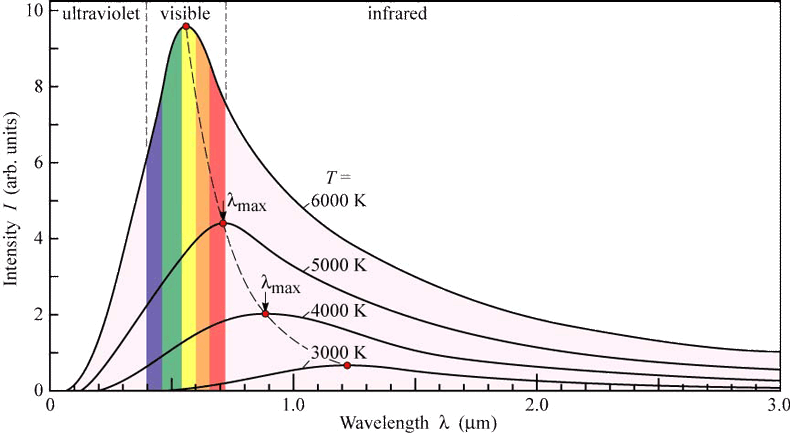
\includegraphics[width=\textwidth]{figures/sampleFig2.png}
    \caption[Black-body radiation ddd dddd dddd]{Spectra of black-body radiation at various temperatures, according to Wien's displacement law \cite{wannier1987statistical}.}
    \label{fig:secondFig}
\end{sidewaysfigure}
\end{rotatepage}

\begin{figure}[ht]
    \centering
	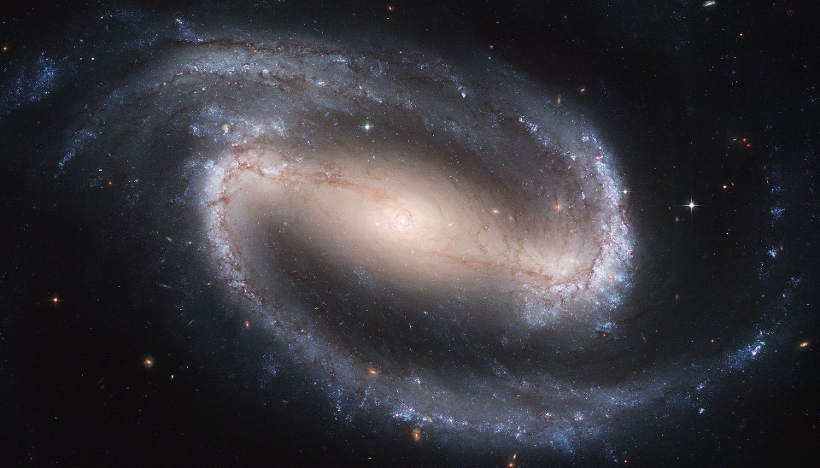
\includegraphics[width=0.85\textwidth]{figures/sampleFig1.jpg} 
	\caption[Barred spiral galaxy NGC 1300]{Barred spiral galaxy NGC 1300 photographed by Hubble telescope. While the galaxy in the photo is not our sun, it does emit light, much like our sun. Image credit: NASA.}
	\label{fig:firstFig}
\end{figure}



%=======================================================%
%%%%% Do not delete this part %%%%%%
\clearpage

\printbibliography[heading=subbibintoc, title={\texorpdfstring{\centering}{} Notes}]
\end{refsection}
    
\chapter{Methodology}
\begin{refsection}
% text of this chapter goes here

\begin{figure}[ht]
    \centering
	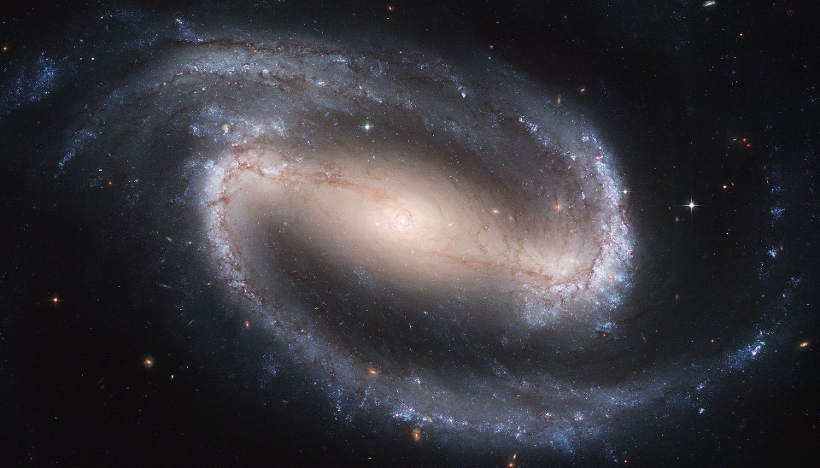
\includegraphics[width=0.85\textwidth]{figures/sampleFig1.jpg} 
	\caption[Barred spiral galaxy NGC 1300]{Barred spiral galaxy NGC 1300 photographed by Hubble telescope. While the galaxy in the photo is not our sun, it does emit light, much like our sun. Image credit: NASA.}
	\label{fig:firstFig}
\end{figure}

%=======================================================%
%%%%% Do not delete this part %%%%%%
\clearpage

\printbibliography[heading=subbibintoc, title={\texorpdfstring{\centering}{} Notes}]
\end{refsection}
    
\chapter{Results and Discussion}

The data gathered during the study are presented and evaluated in this chapter. A discussion and thorough analysis of helmet compliance, wrong helmet use, and motorcycle overloading are also included in this chapter.
\begin{refsection}

\section{Data Collection}
\subsection{Data Gathering}
The researchers searched for datasets that included motorcycles, not motorcycles, persons with no helmet, persons with proper helmets, and persons with wrong helmet use. While it was easy to find images for motorcycles, not motorcycles, no-helmet, and proper-helmet categories, finding enough images for wrong helmet use was challenging. To create the dataset, the researchers used a phone to capture images of riders and used some images from the internet. In total, the dataset consists of around 1,133 images covering all categories. Before training the model, the images were preprocessed. This included resizing all images to a standard input size, labeling each image with bounding boxes for motorcycles and riders, and applying data augmentation techniques such as flipping, blurring, rotation, brightness adjustment, adding noise, and cropping to increase variability. The pixel values of the images were normalized to improve model training, and the dataset was split into training, validation, and test sets to allow proper evaluation of the model’s performance.

\begin{figure}[H]
\centering
\begin{tabular}{|c|c|c|}
\hline
Motorcycle & Not motorcycle & Person with no helmet \\
\hline
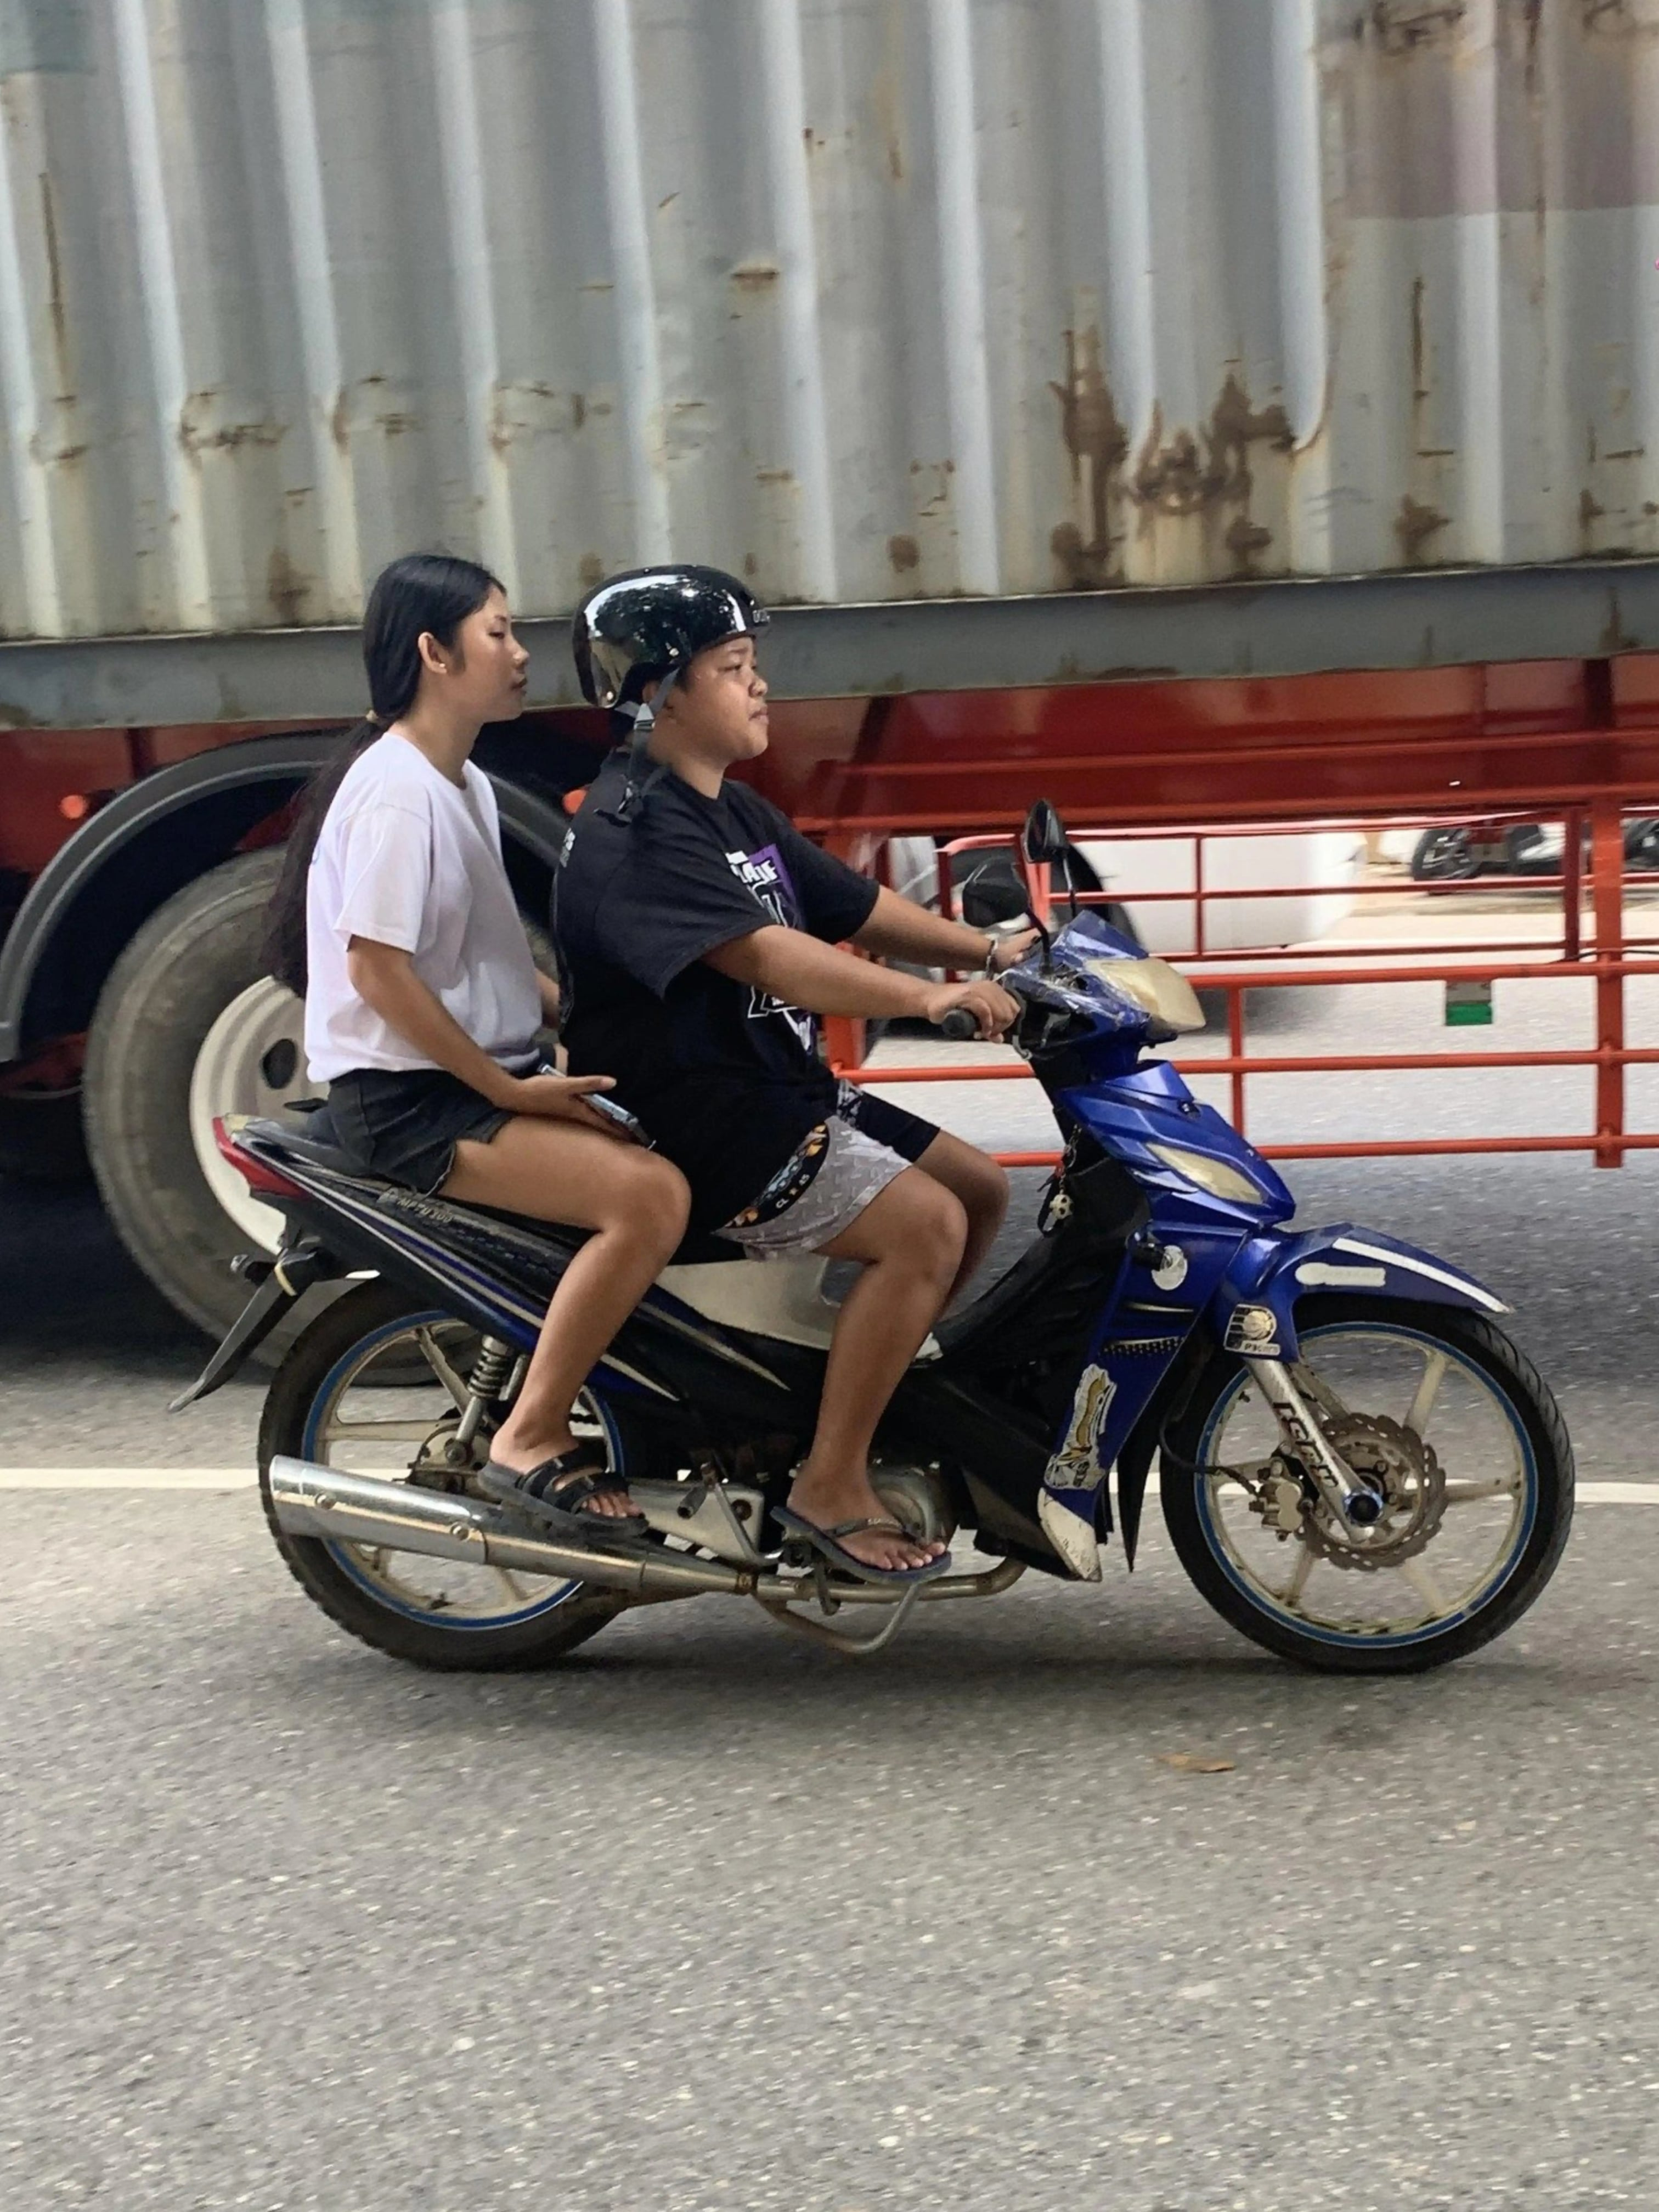
\includegraphics[width=0.28\textwidth]{figures/Fig 7.png} & 
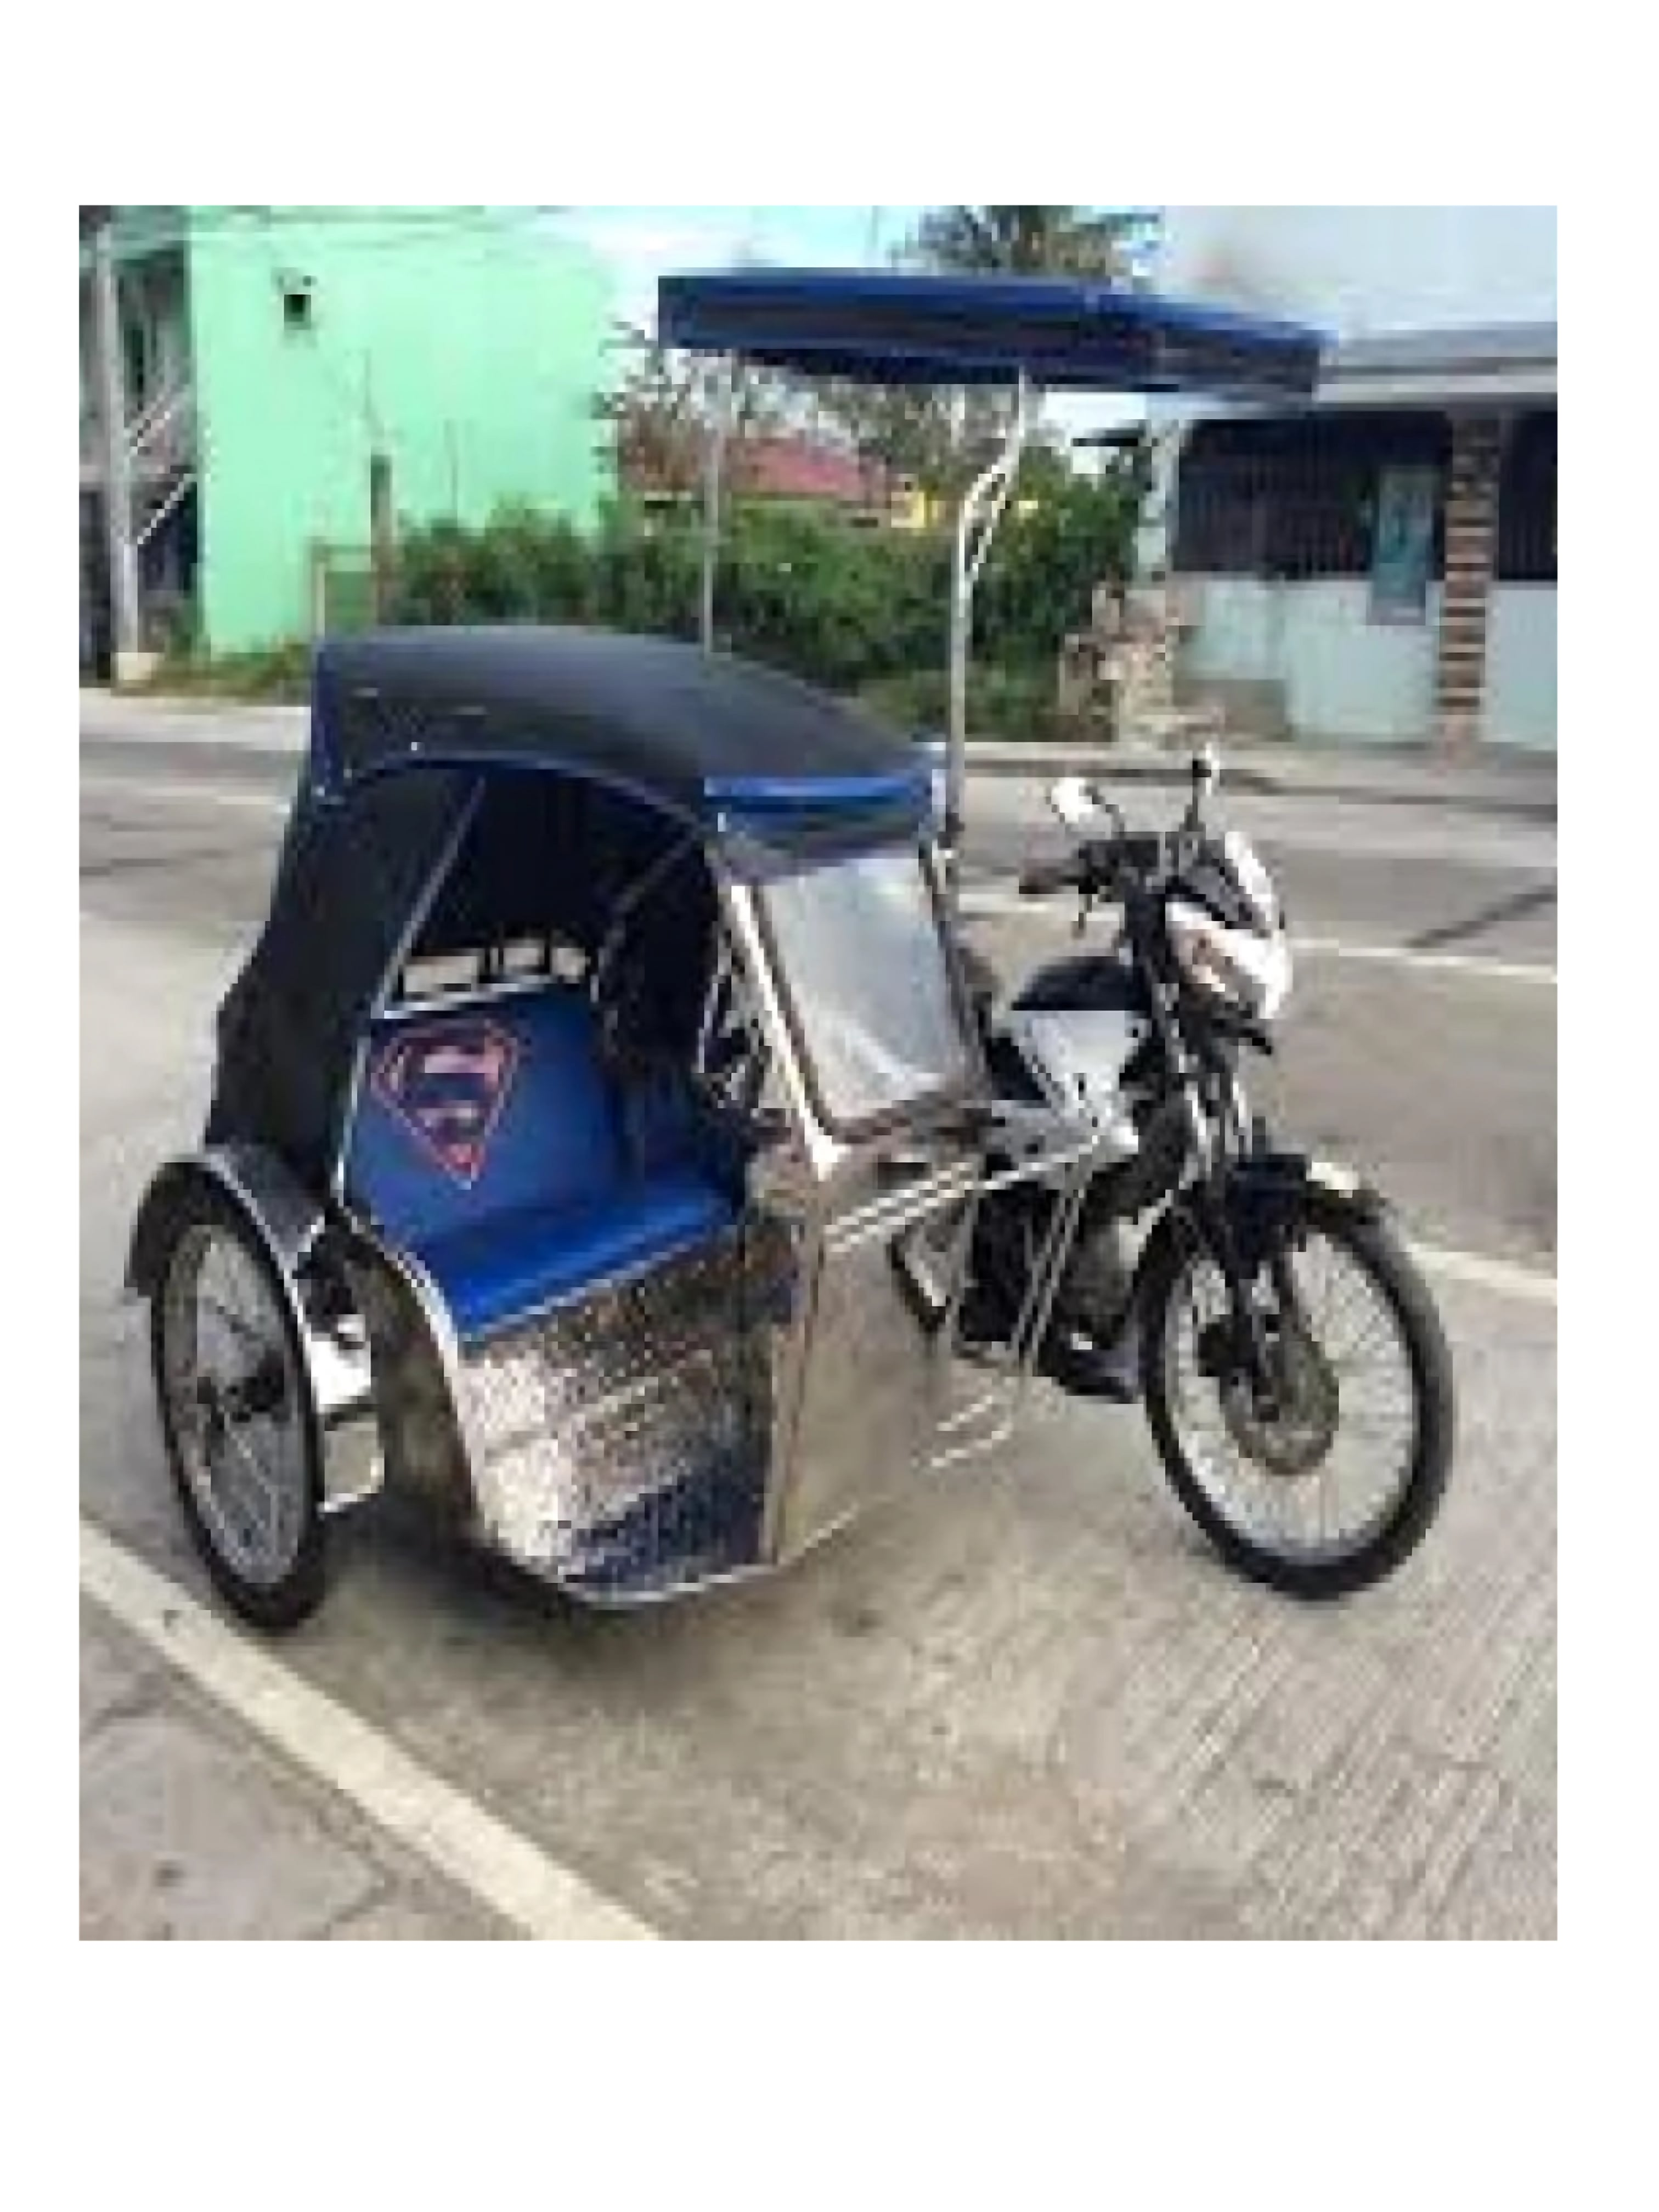
\includegraphics[width=0.28\textwidth]{figures/Fig 8.png} & 
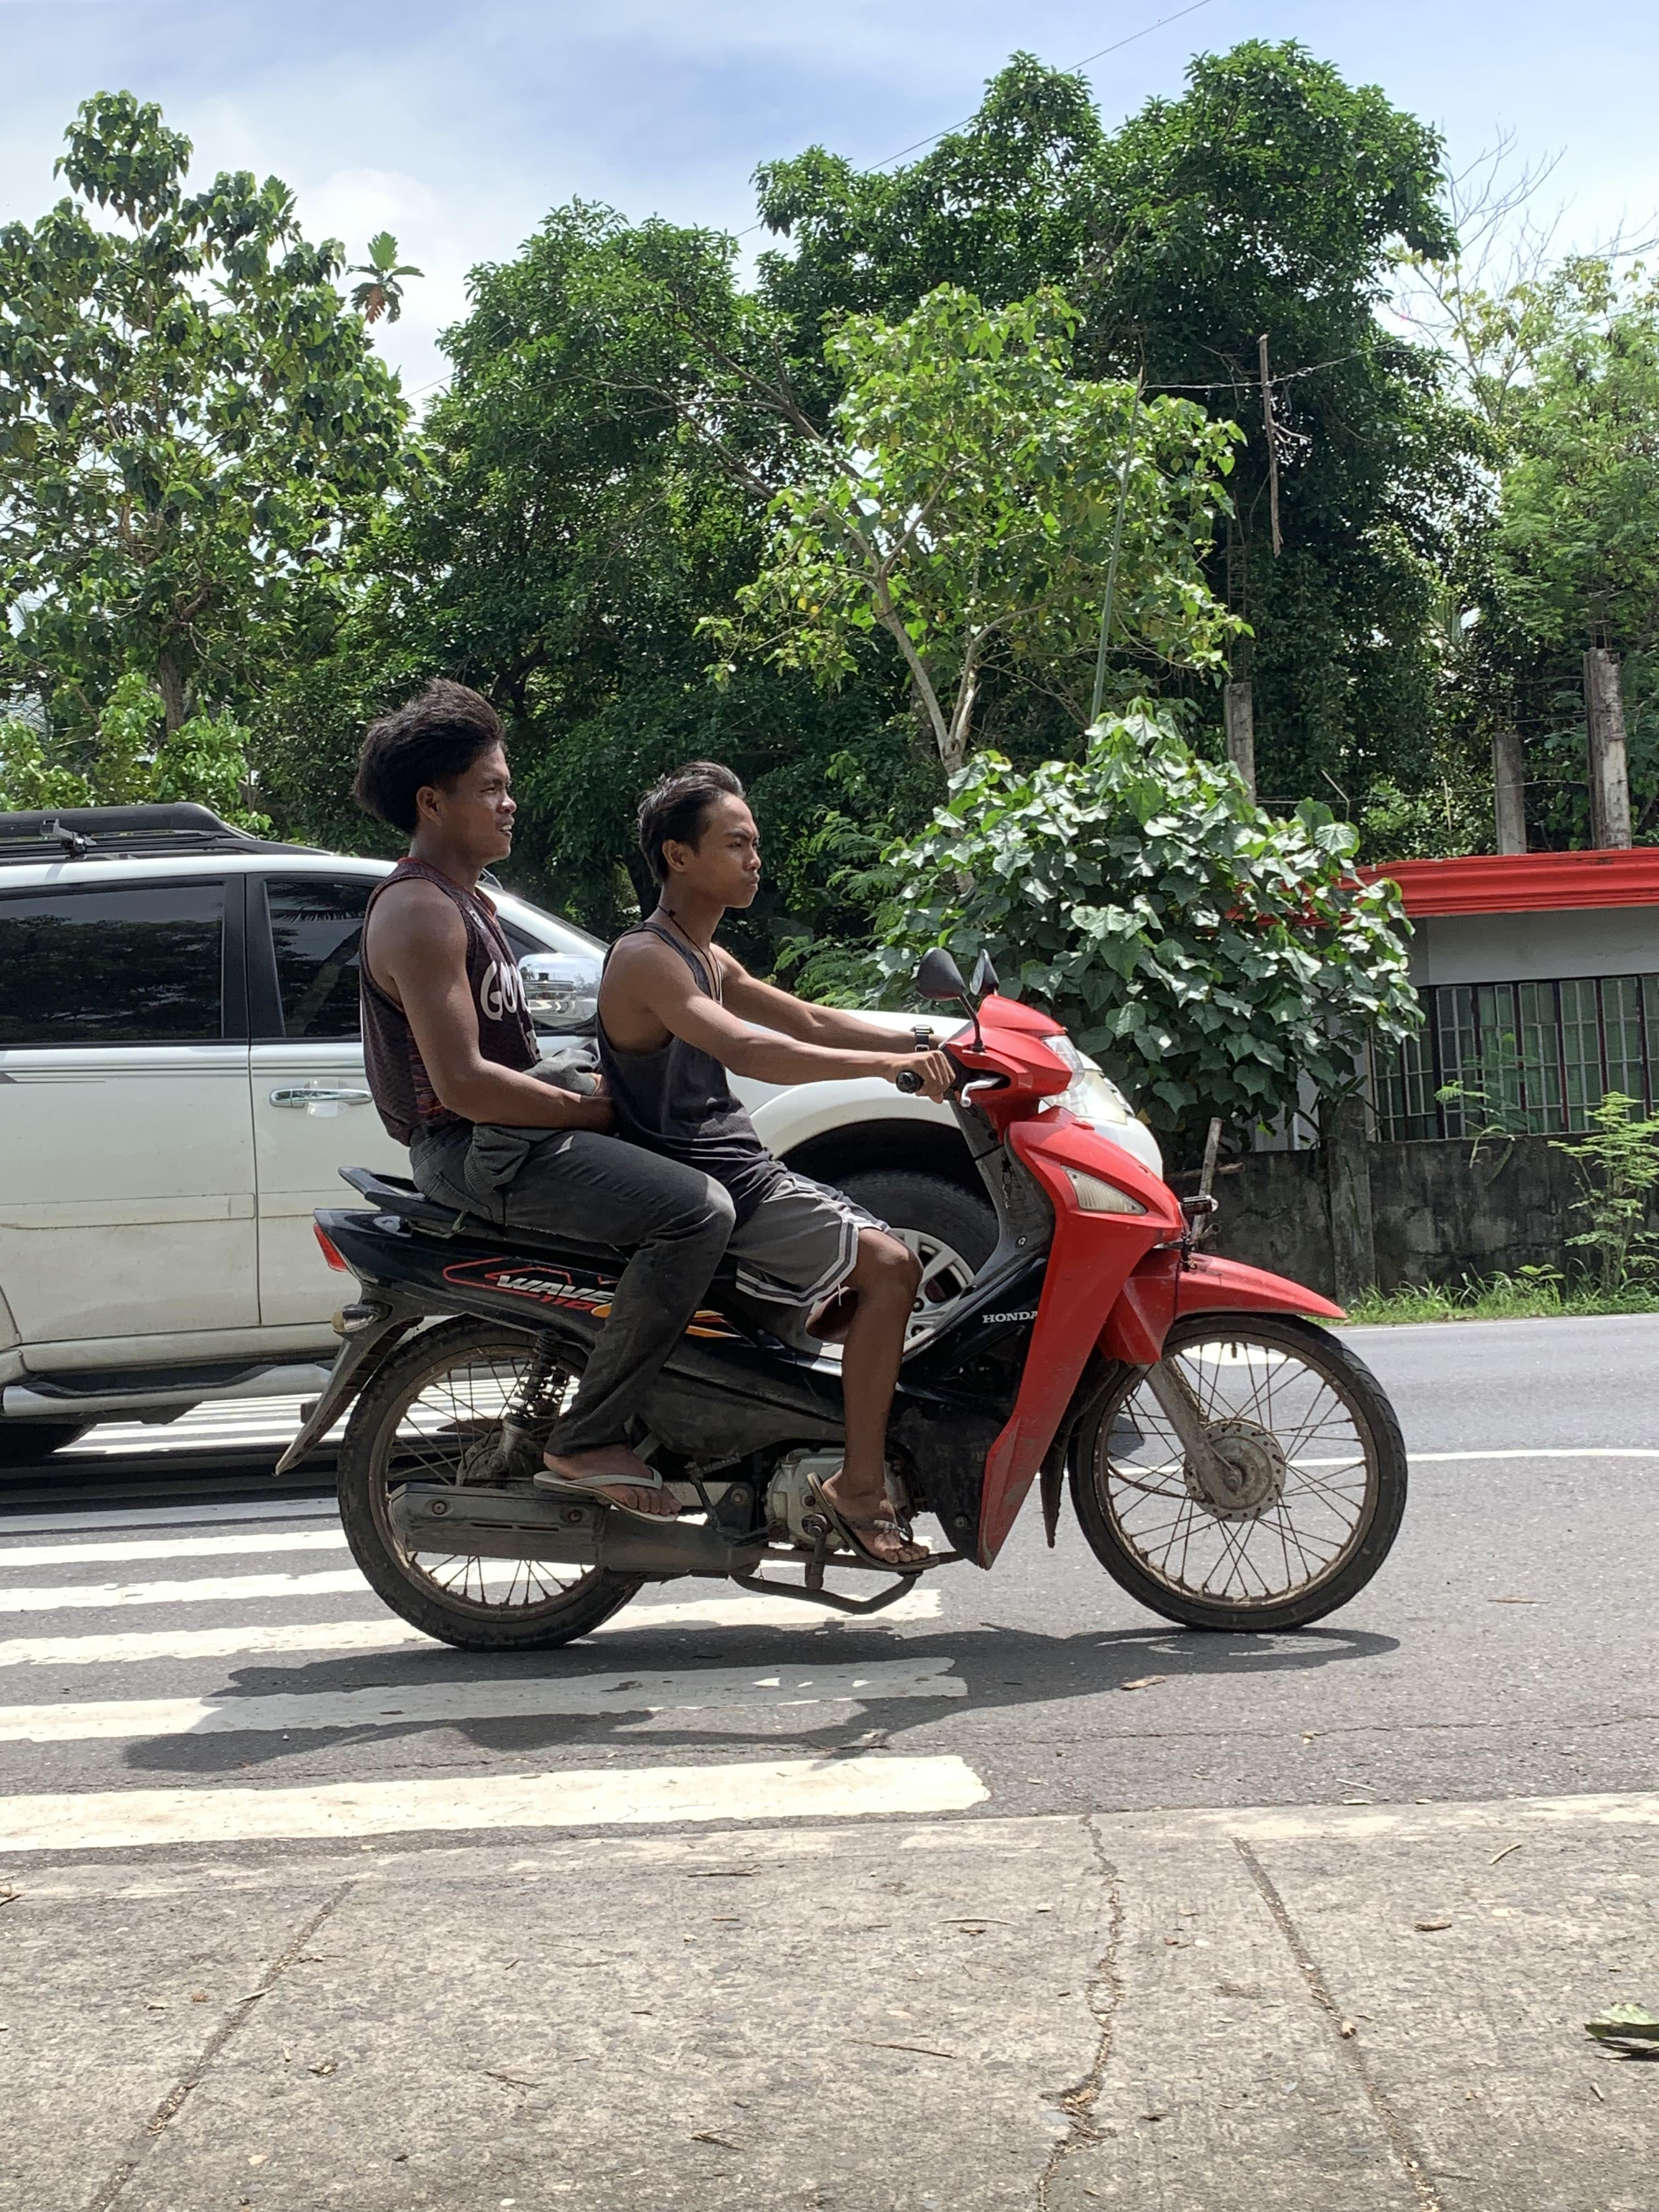
\includegraphics[width=0.28\textwidth]{figures/Fig 9.png} \\
\hline
\end{tabular}

\vspace{0.3cm} % space between rows

\begin{tabular}{|c|c|}
\hline
Person with proper helmet & Person with wrong helmet use \\
\hline
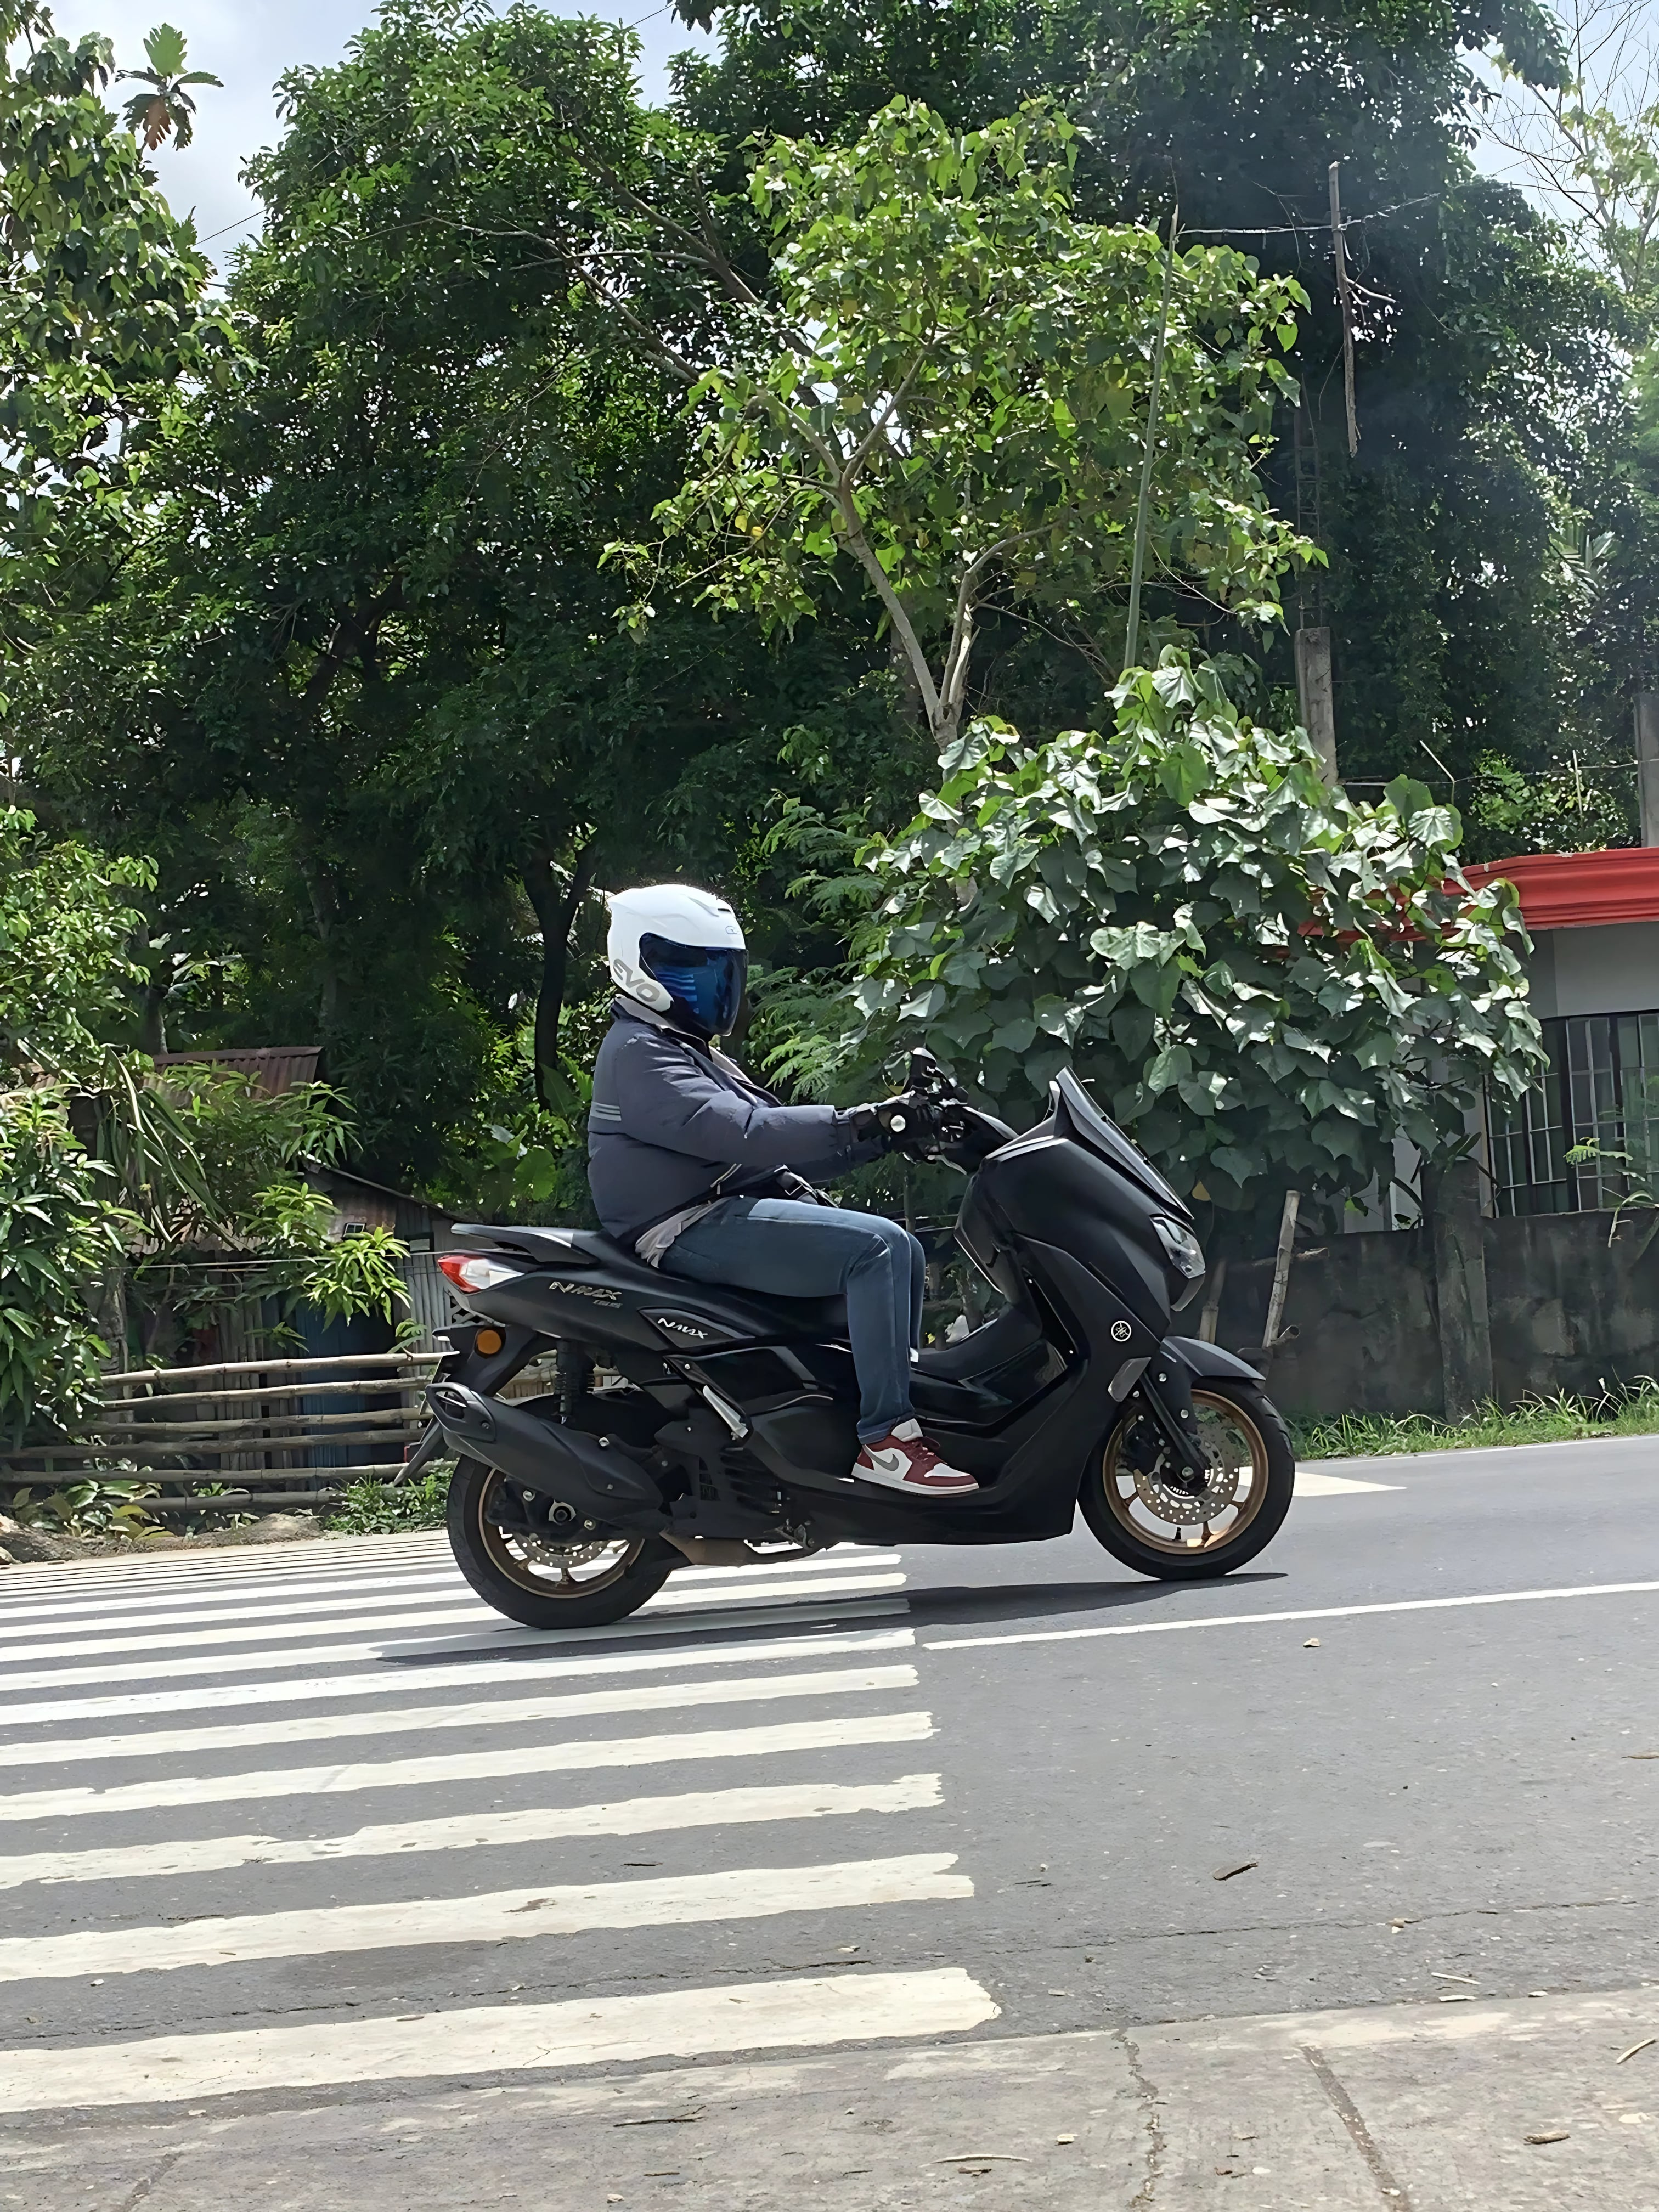
\includegraphics[width=0.35\textwidth]{figures/Fig 10.png} & 
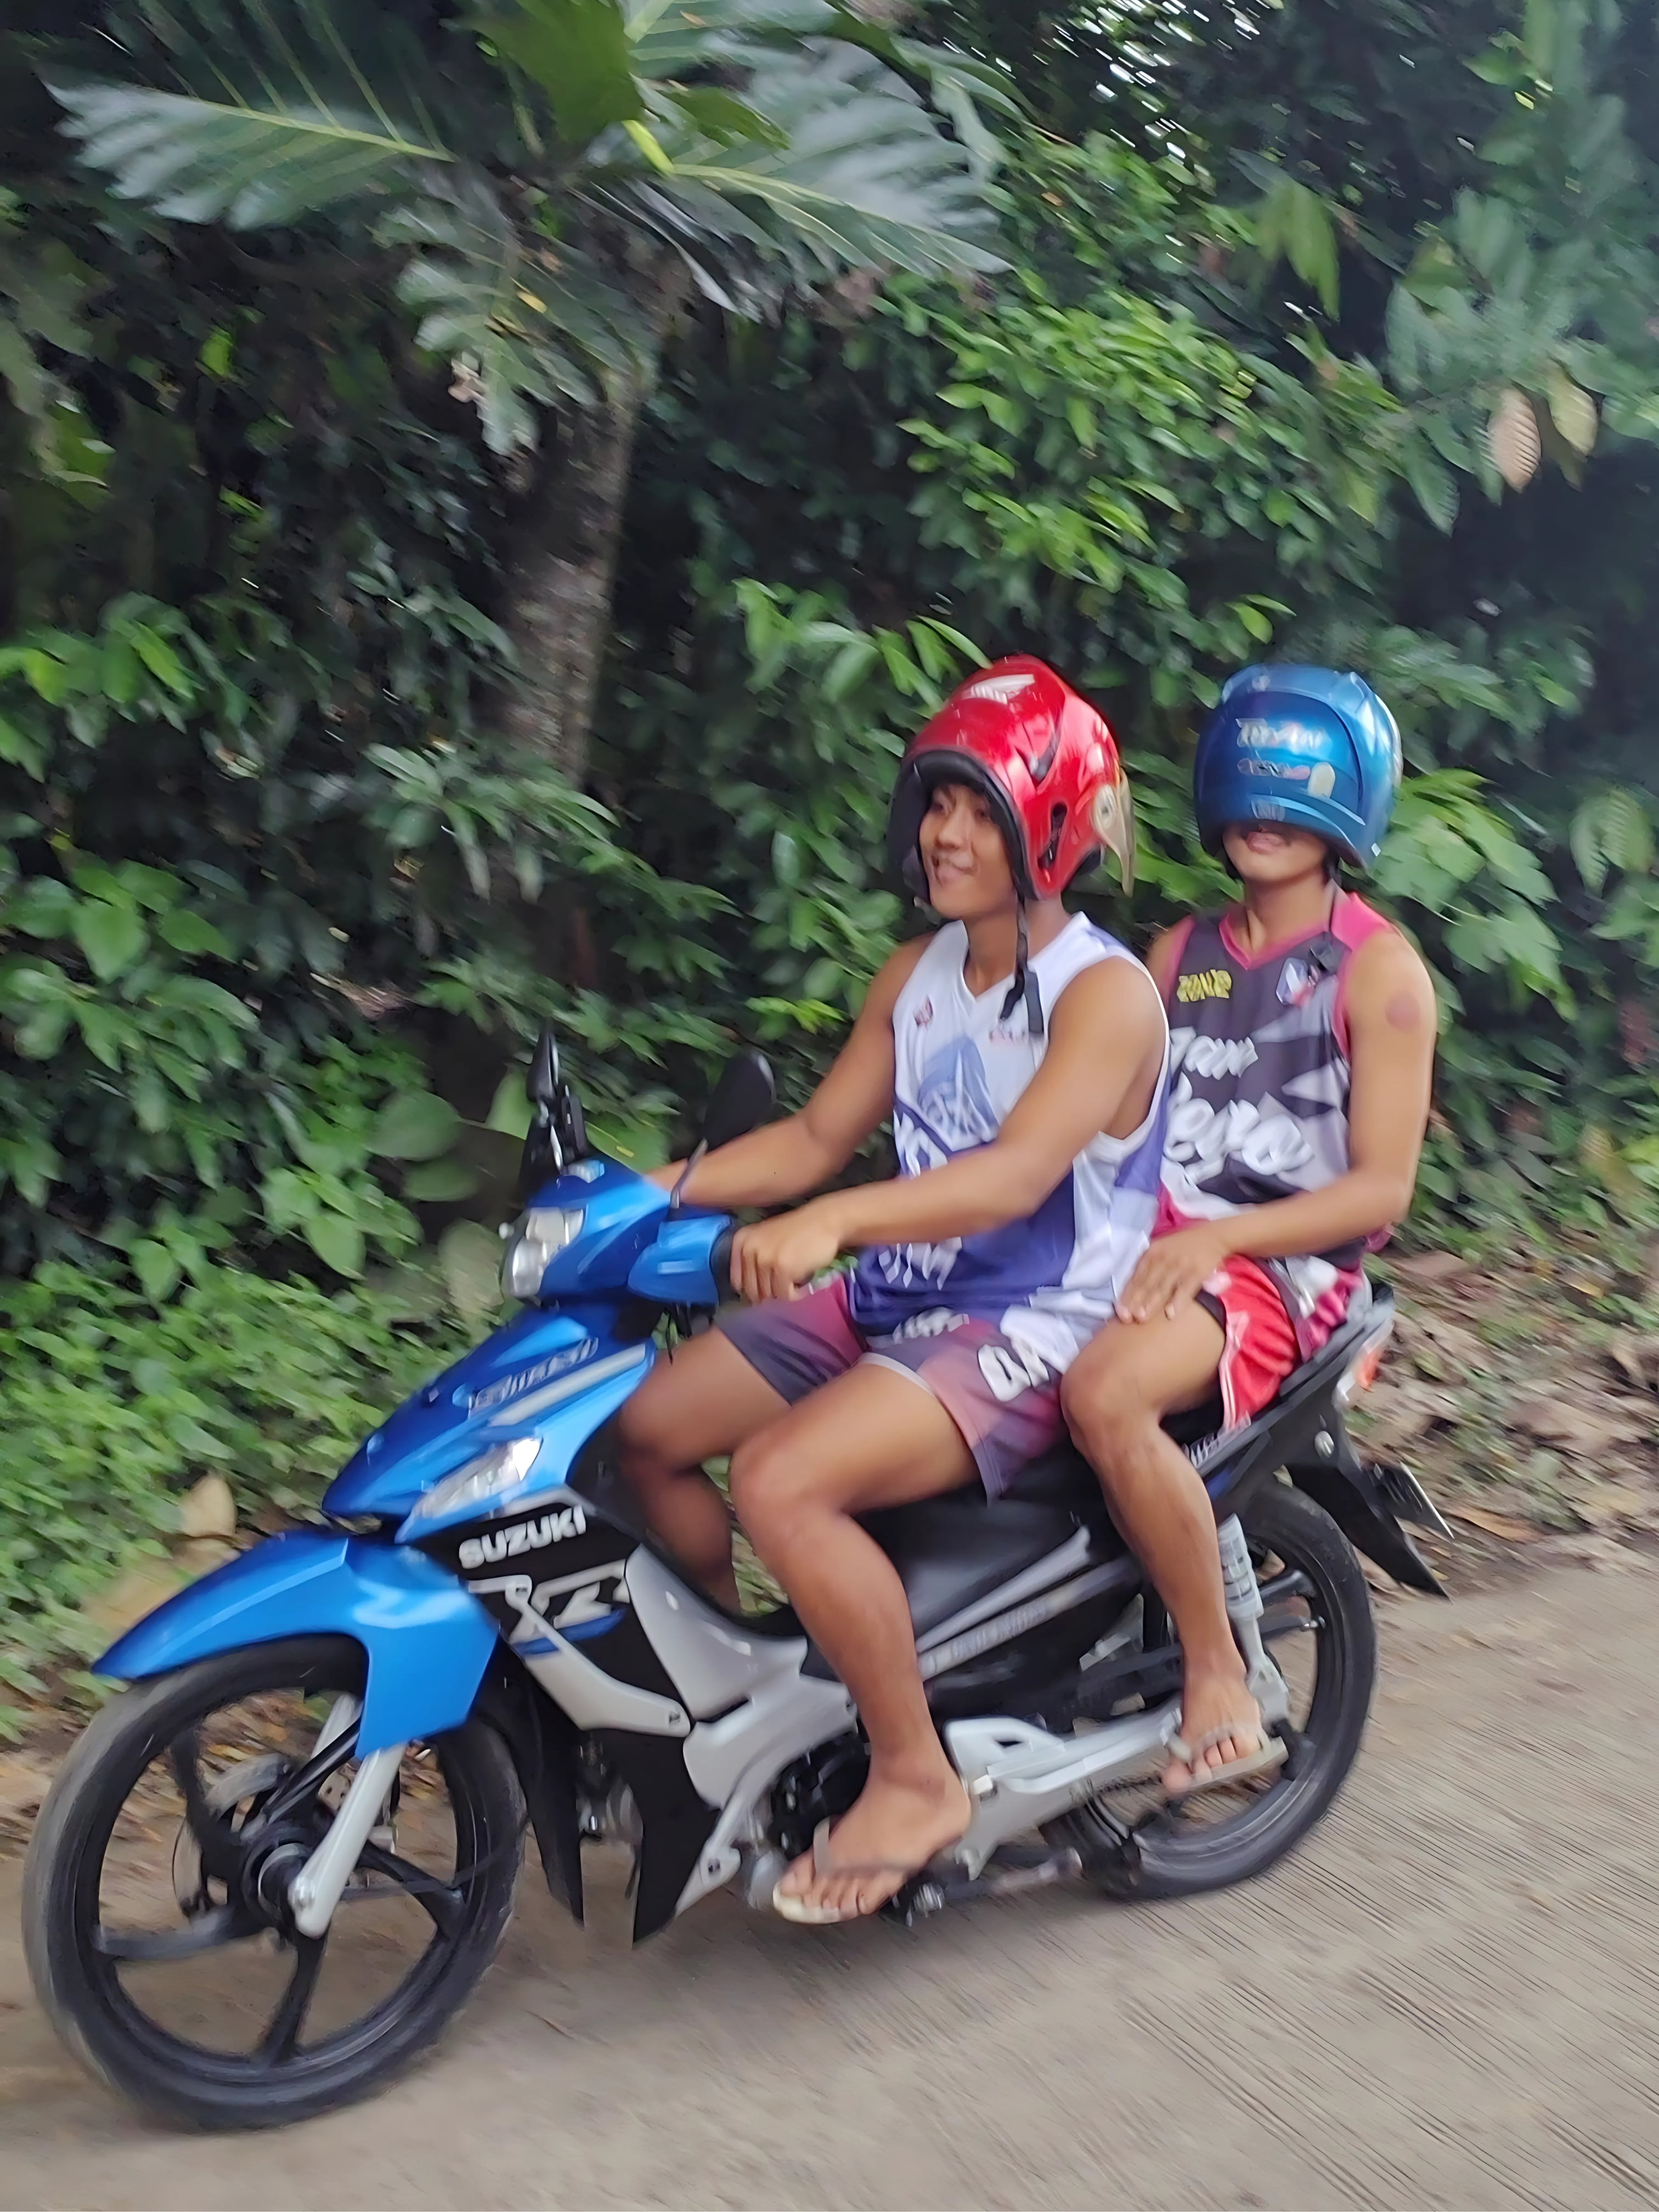
\includegraphics[width=0.35\textwidth]{figures/Fig 11.png} \\
\hline
\end{tabular}

\caption{Examples of Datasets.}
\label{fig:helmet_classification}
\end{figure}

\subsection{Data Pre-Processing}

\begin{figure}[ht]
    \centering
	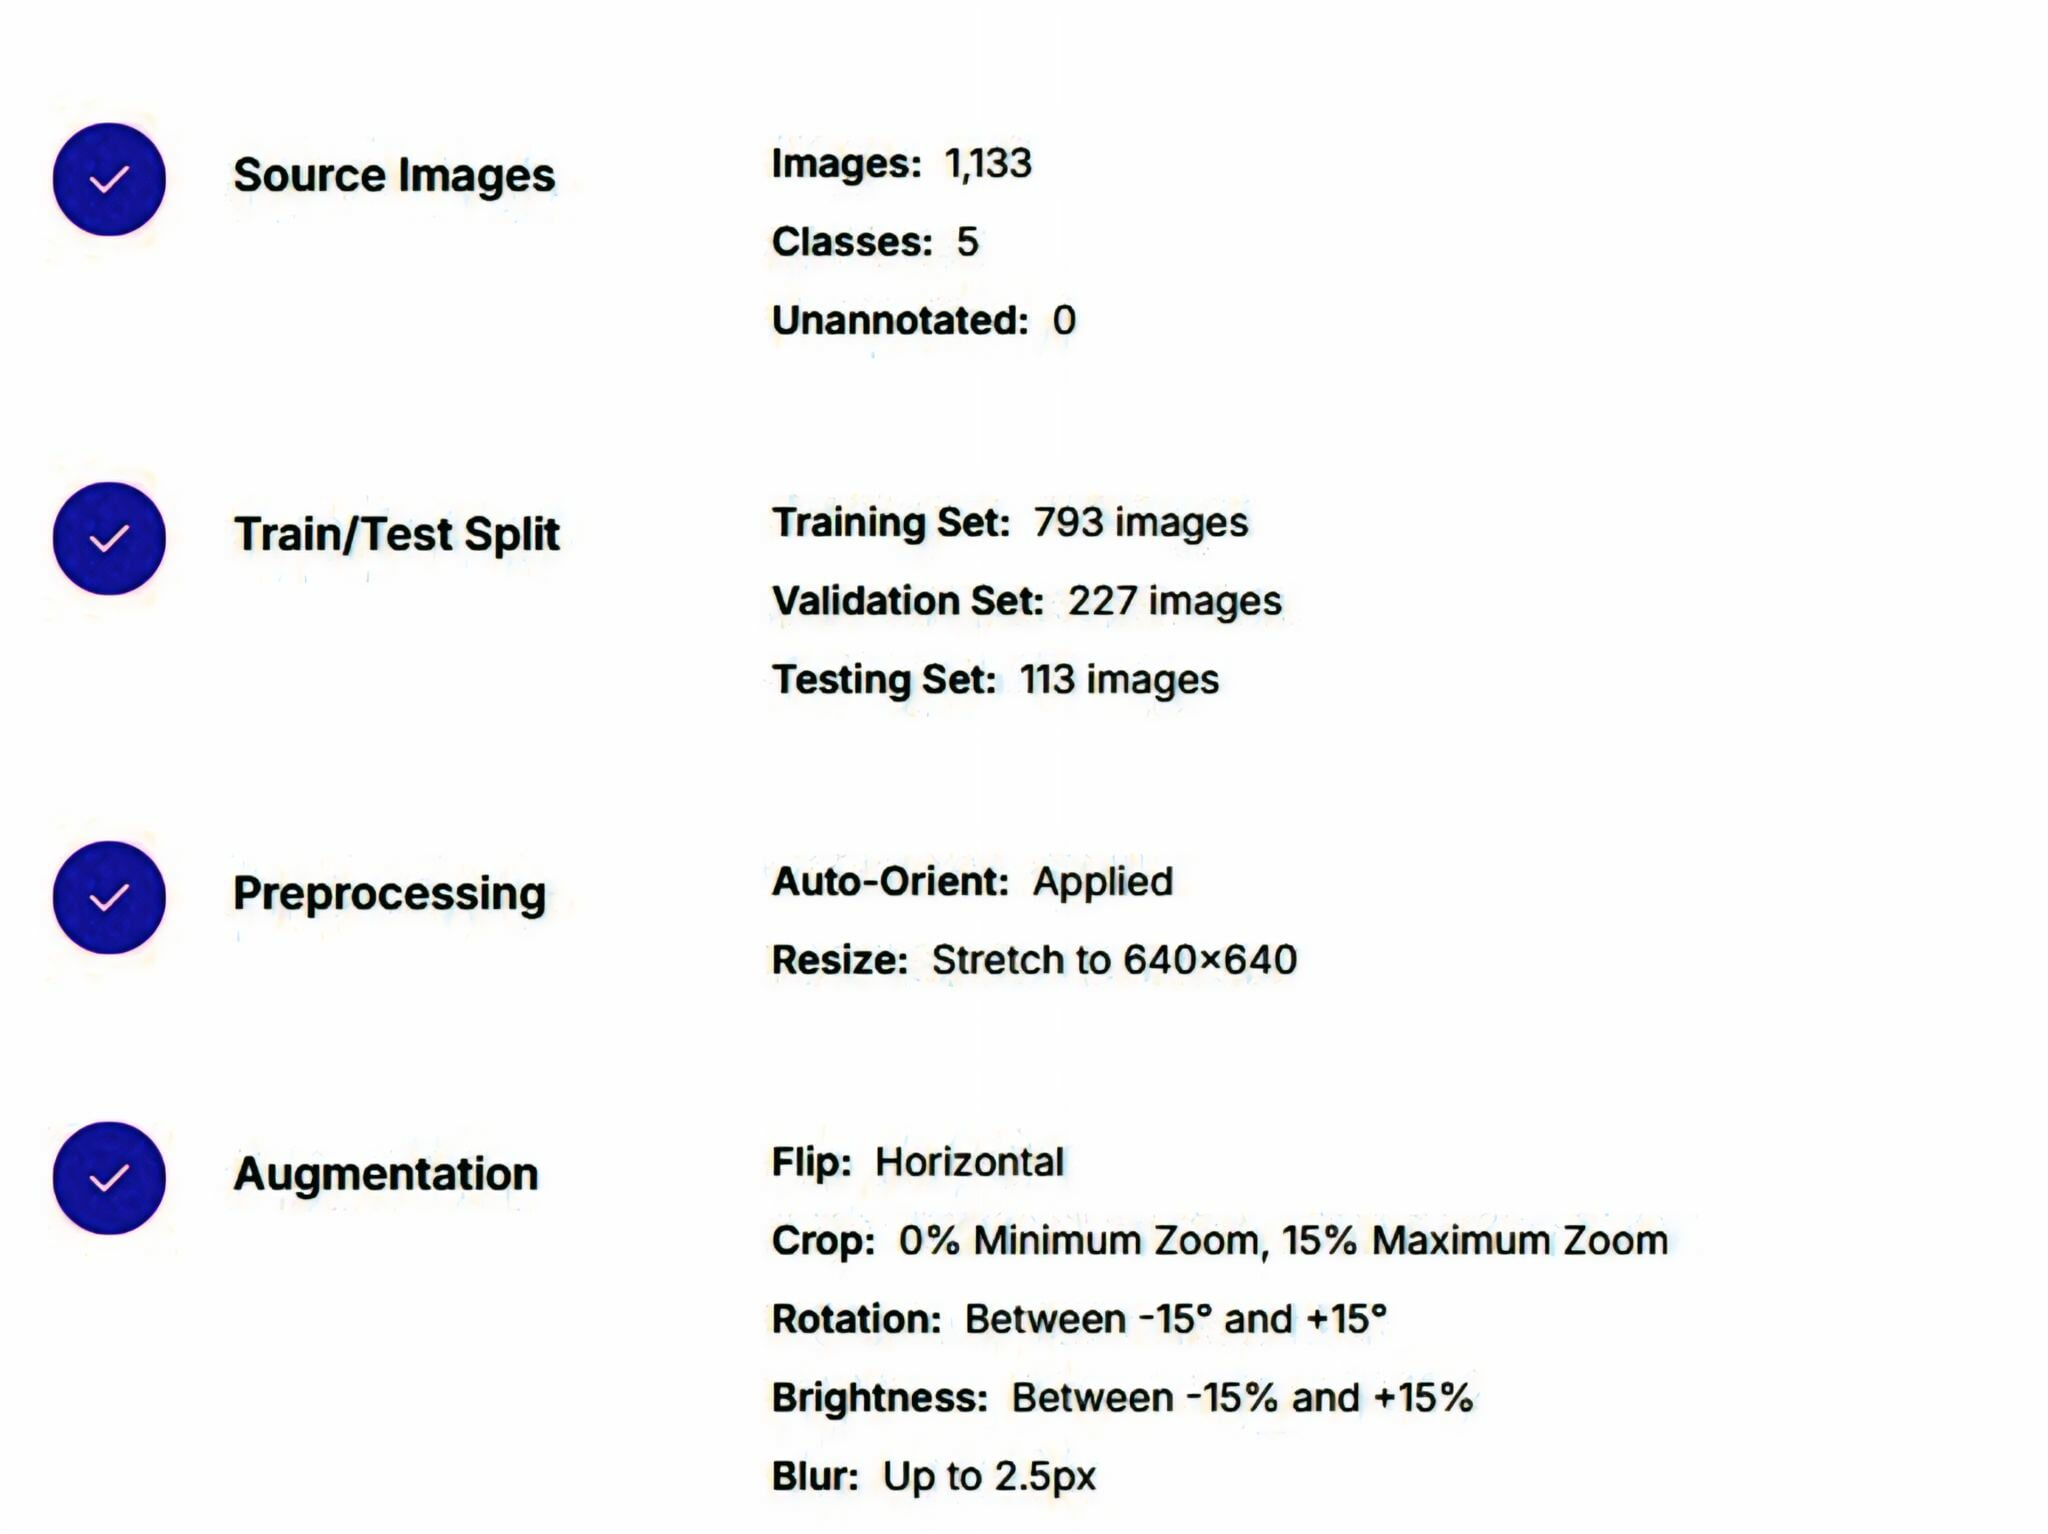
\includegraphics[width=0.85\textwidth]{figures/Fig 12.jpg}
	\caption[Data Pre-processing]{Data Pre-processing}
	\label{fig:data_preprocessing}
\end{figure}

A total of 1,133 images were collected and fully processed using Roboflow, where they were uploaded, annotated into five classes relevant to helmet compliance detection, and organized into a complete dataset. All images were properly labeled, ensuring no unannotated data remained. To support effective model training and evaluation, the dataset was divided into 793 images for training, 227 for validation, and 113 for testing. This split allowed the model to learn from the majority of the data while its accuracy was assessed on separate validation and testing sets.

In Roboflow, the images were preprocessed by applying auto-orientation to correct rotation errors and resizing them to 640×640 pixels, the standard input size required by the YOLOv8 model. To improve model performance and adaptability to real-world scenarios, several data augmentation techniques were applied. These included horizontal flipping to simulate different orientations, random cropping of up to 15\% to represent objects at varying distances, rotation adjustments between -15° and +15° to account for tilted camera angles, brightness variations of ±15\% to handle different lighting conditions, and blurring of up to 2.5 pixels to increase resilience to motion blur. These preprocessing and augmentation steps enriched the dataset, enabling the YOLOv8 model to generalize better and perform more reliably during testing and deployment.

\section{Model Training and Evaluation}
\noindent
The model was trained using a dataset with five classes: motorcycle, not motorcycle, person with no helmet, person with proper helmet, and person with wrong helmet use. The dataset was divided into training, validation, and test sets to evaluate the model. Before training, images were resized, normalized, and augmented using flipping, blurring, rotation, brightness changes, noise, and cropping to improve learning. The model was trained with the YOLOv8 algorithm for 150 epochs using batch processing, which allowed many images to be processed at once. It learned to detect and classify objects using the labeled bounding boxes. The model’s performance was measured using precision, recall, F1-score, and mean Average Precision (mAP) to show how accurately it detects helmet use and violations.

\begin{figure}[ht]
    \centering
	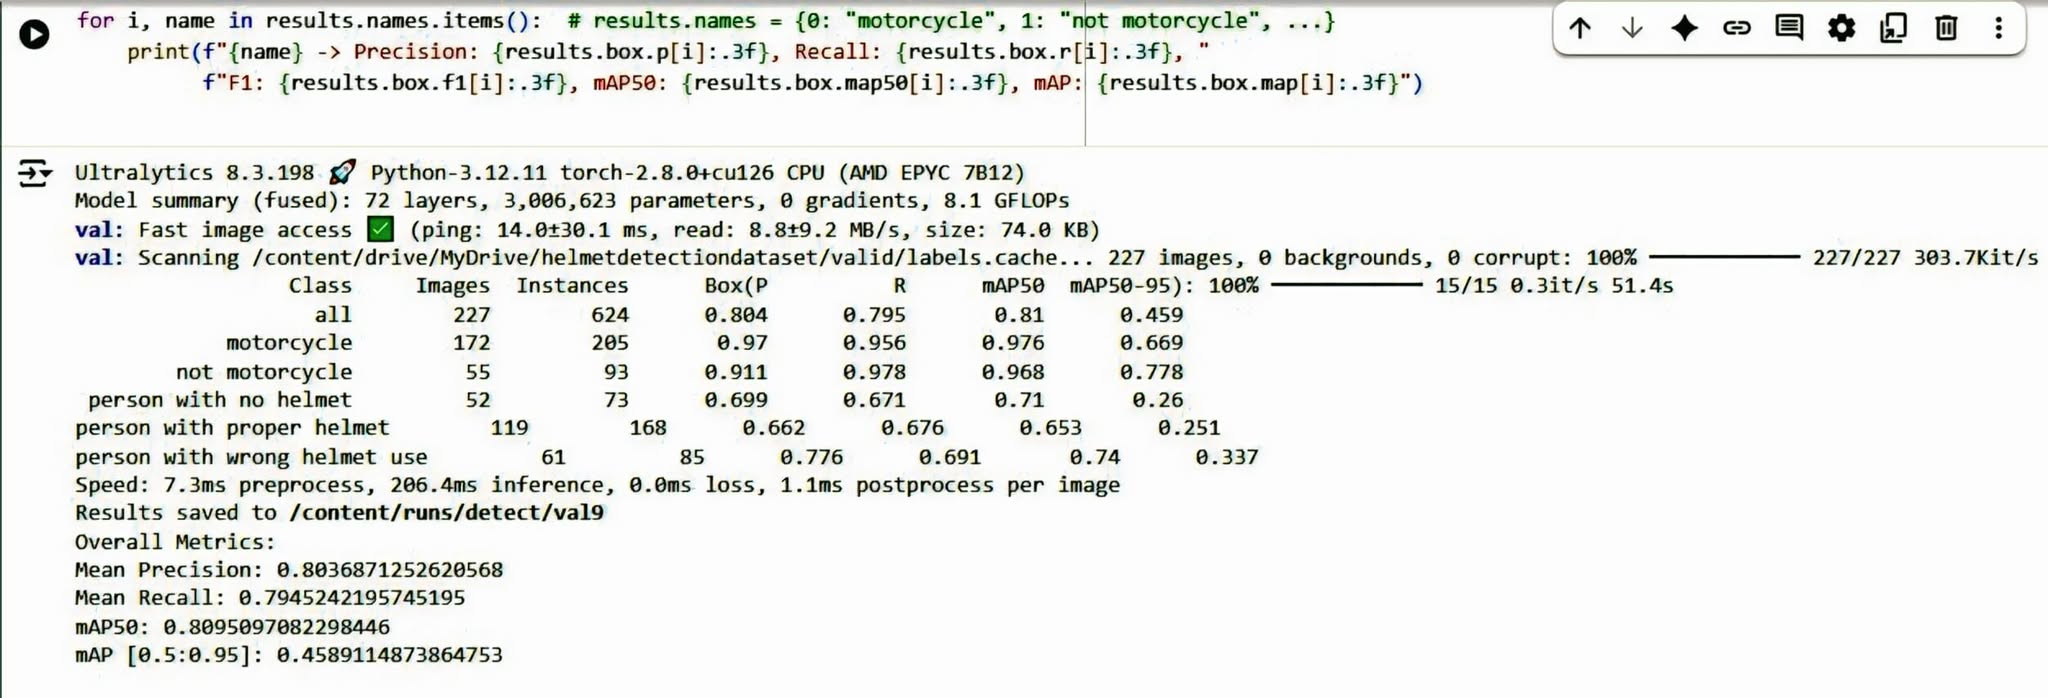
\includegraphics[width=0.85\textwidth]{figures/Fig 13.jpg}
	\caption[Model Training]{Model Training}
	\label{fig:model_training}
\end{figure}

\subsubsection{Model Evaluation}
\begin{figure}[ht]
    \centering
	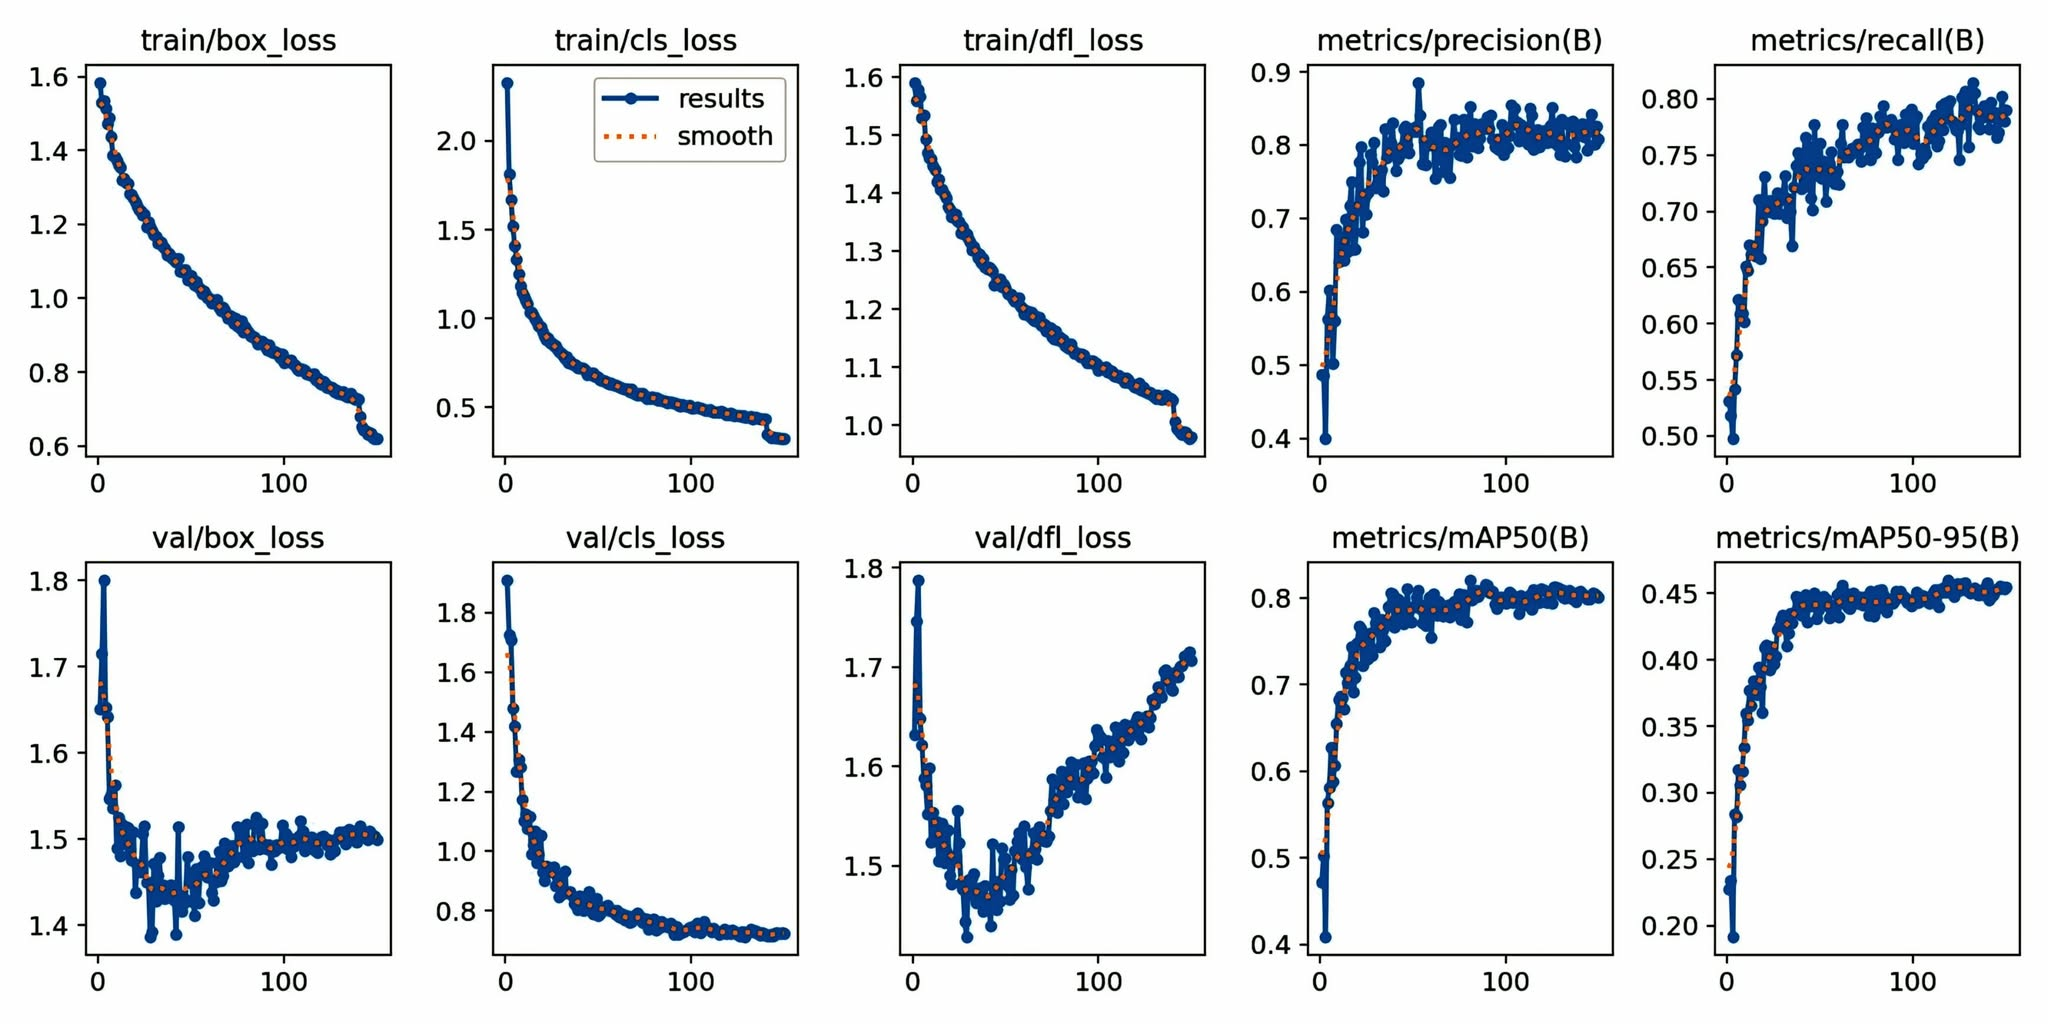
\includegraphics[width=0.85\textwidth]{figures/Fig 14.jpg}
	\caption[Model Evaluation]{Model Evaluation}
	\label{fig:model_evaluation}
\end{figure}

\noindent
Model evaluation results showing per-class performance on the validation dataset. The model achieved high precision and recall for detecting motorcycles, while helmet-related classes (“person with no helmet,” “person with proper helmet,” and “person with wrong helmet use”) had moderate performance. Overall mean precision and recall were approximately 80\%, with mAP50 at 0.81 and mAP@[0.5:0.95] at 0.46, indicating that the model is effective in identifying helmet compliance but has more difficulty with strict detection of helmet violations.

\subsubsection{Training Results}
\begin{figure}[ht]
    \centering
	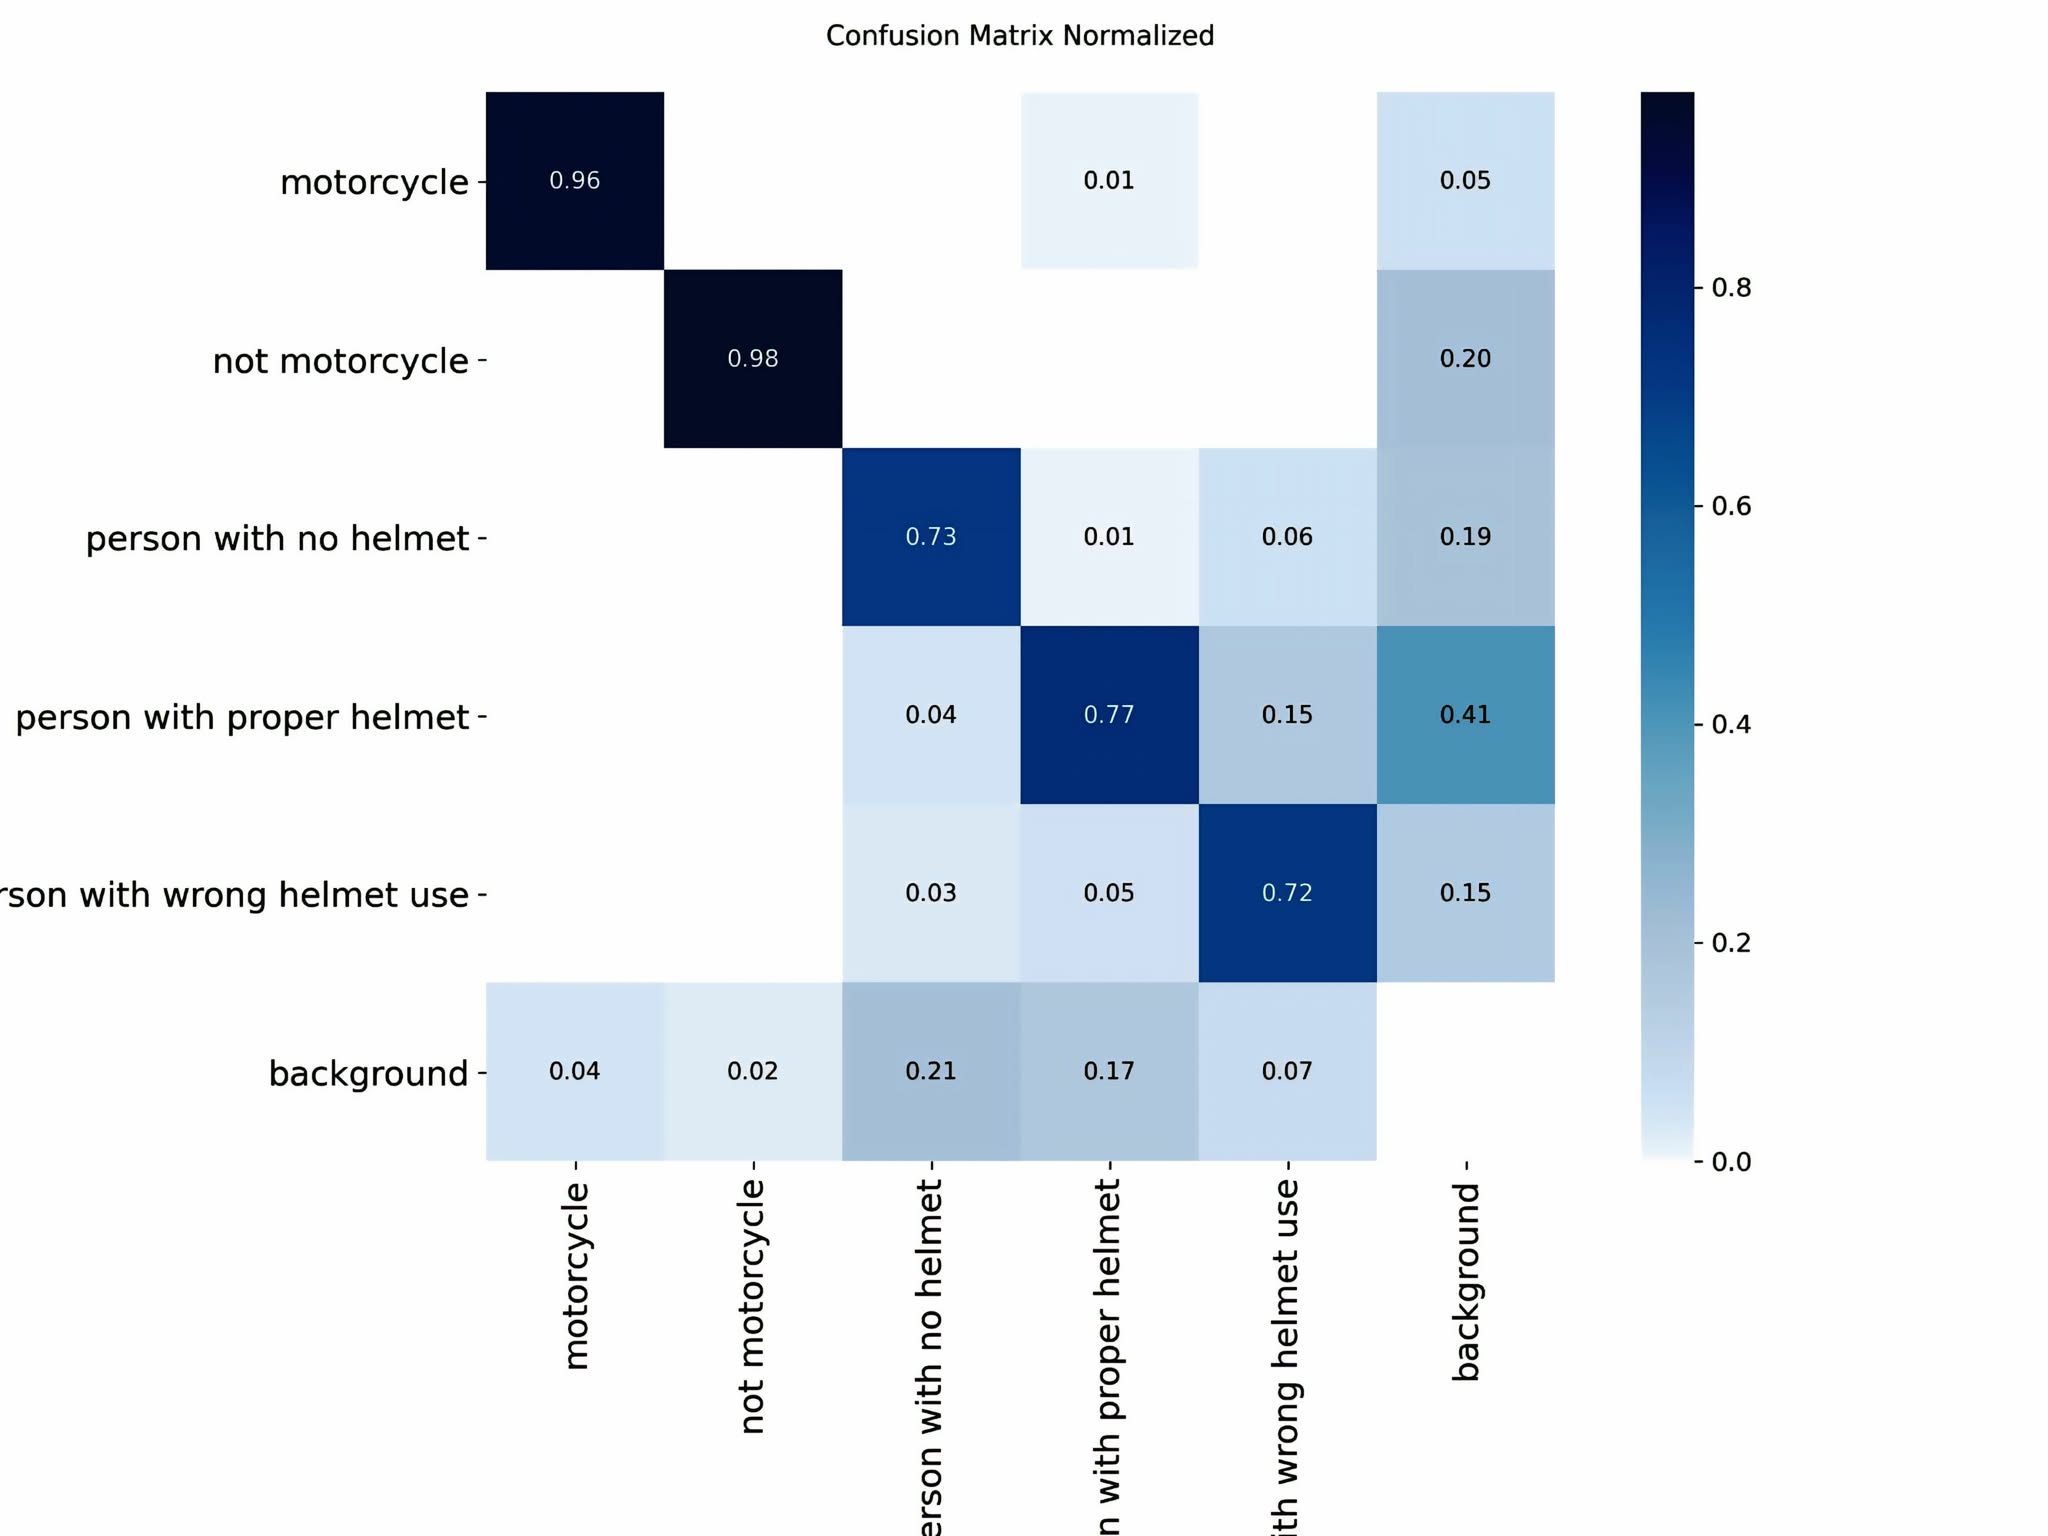
\includegraphics[width=0.85\textwidth]{figures/Fig 15.jpg}
	\caption[Training Results]{Training Results}
	\label{fig:training_results}
\end{figure}

\noindent
The training results show that the model learned effectively as the box, classification, and DFL losses decreased over time. Both precision and recall stabilized around 0.8, which means the model is good at correctly detecting objects and finding most of them. For overall detection performance, the model achieved about 0.8 mAP@50 and 0.45 mAP@50-95, showing strong accuracy though performance decreases under stricter evaluation. Validation results also suggest minor signs of overfitting, but the model still demonstrates reliable performance in identifying and classifying objects.

\subsubsection{Confusion Matrix}
\begin{figure}[ht]
    \centering
	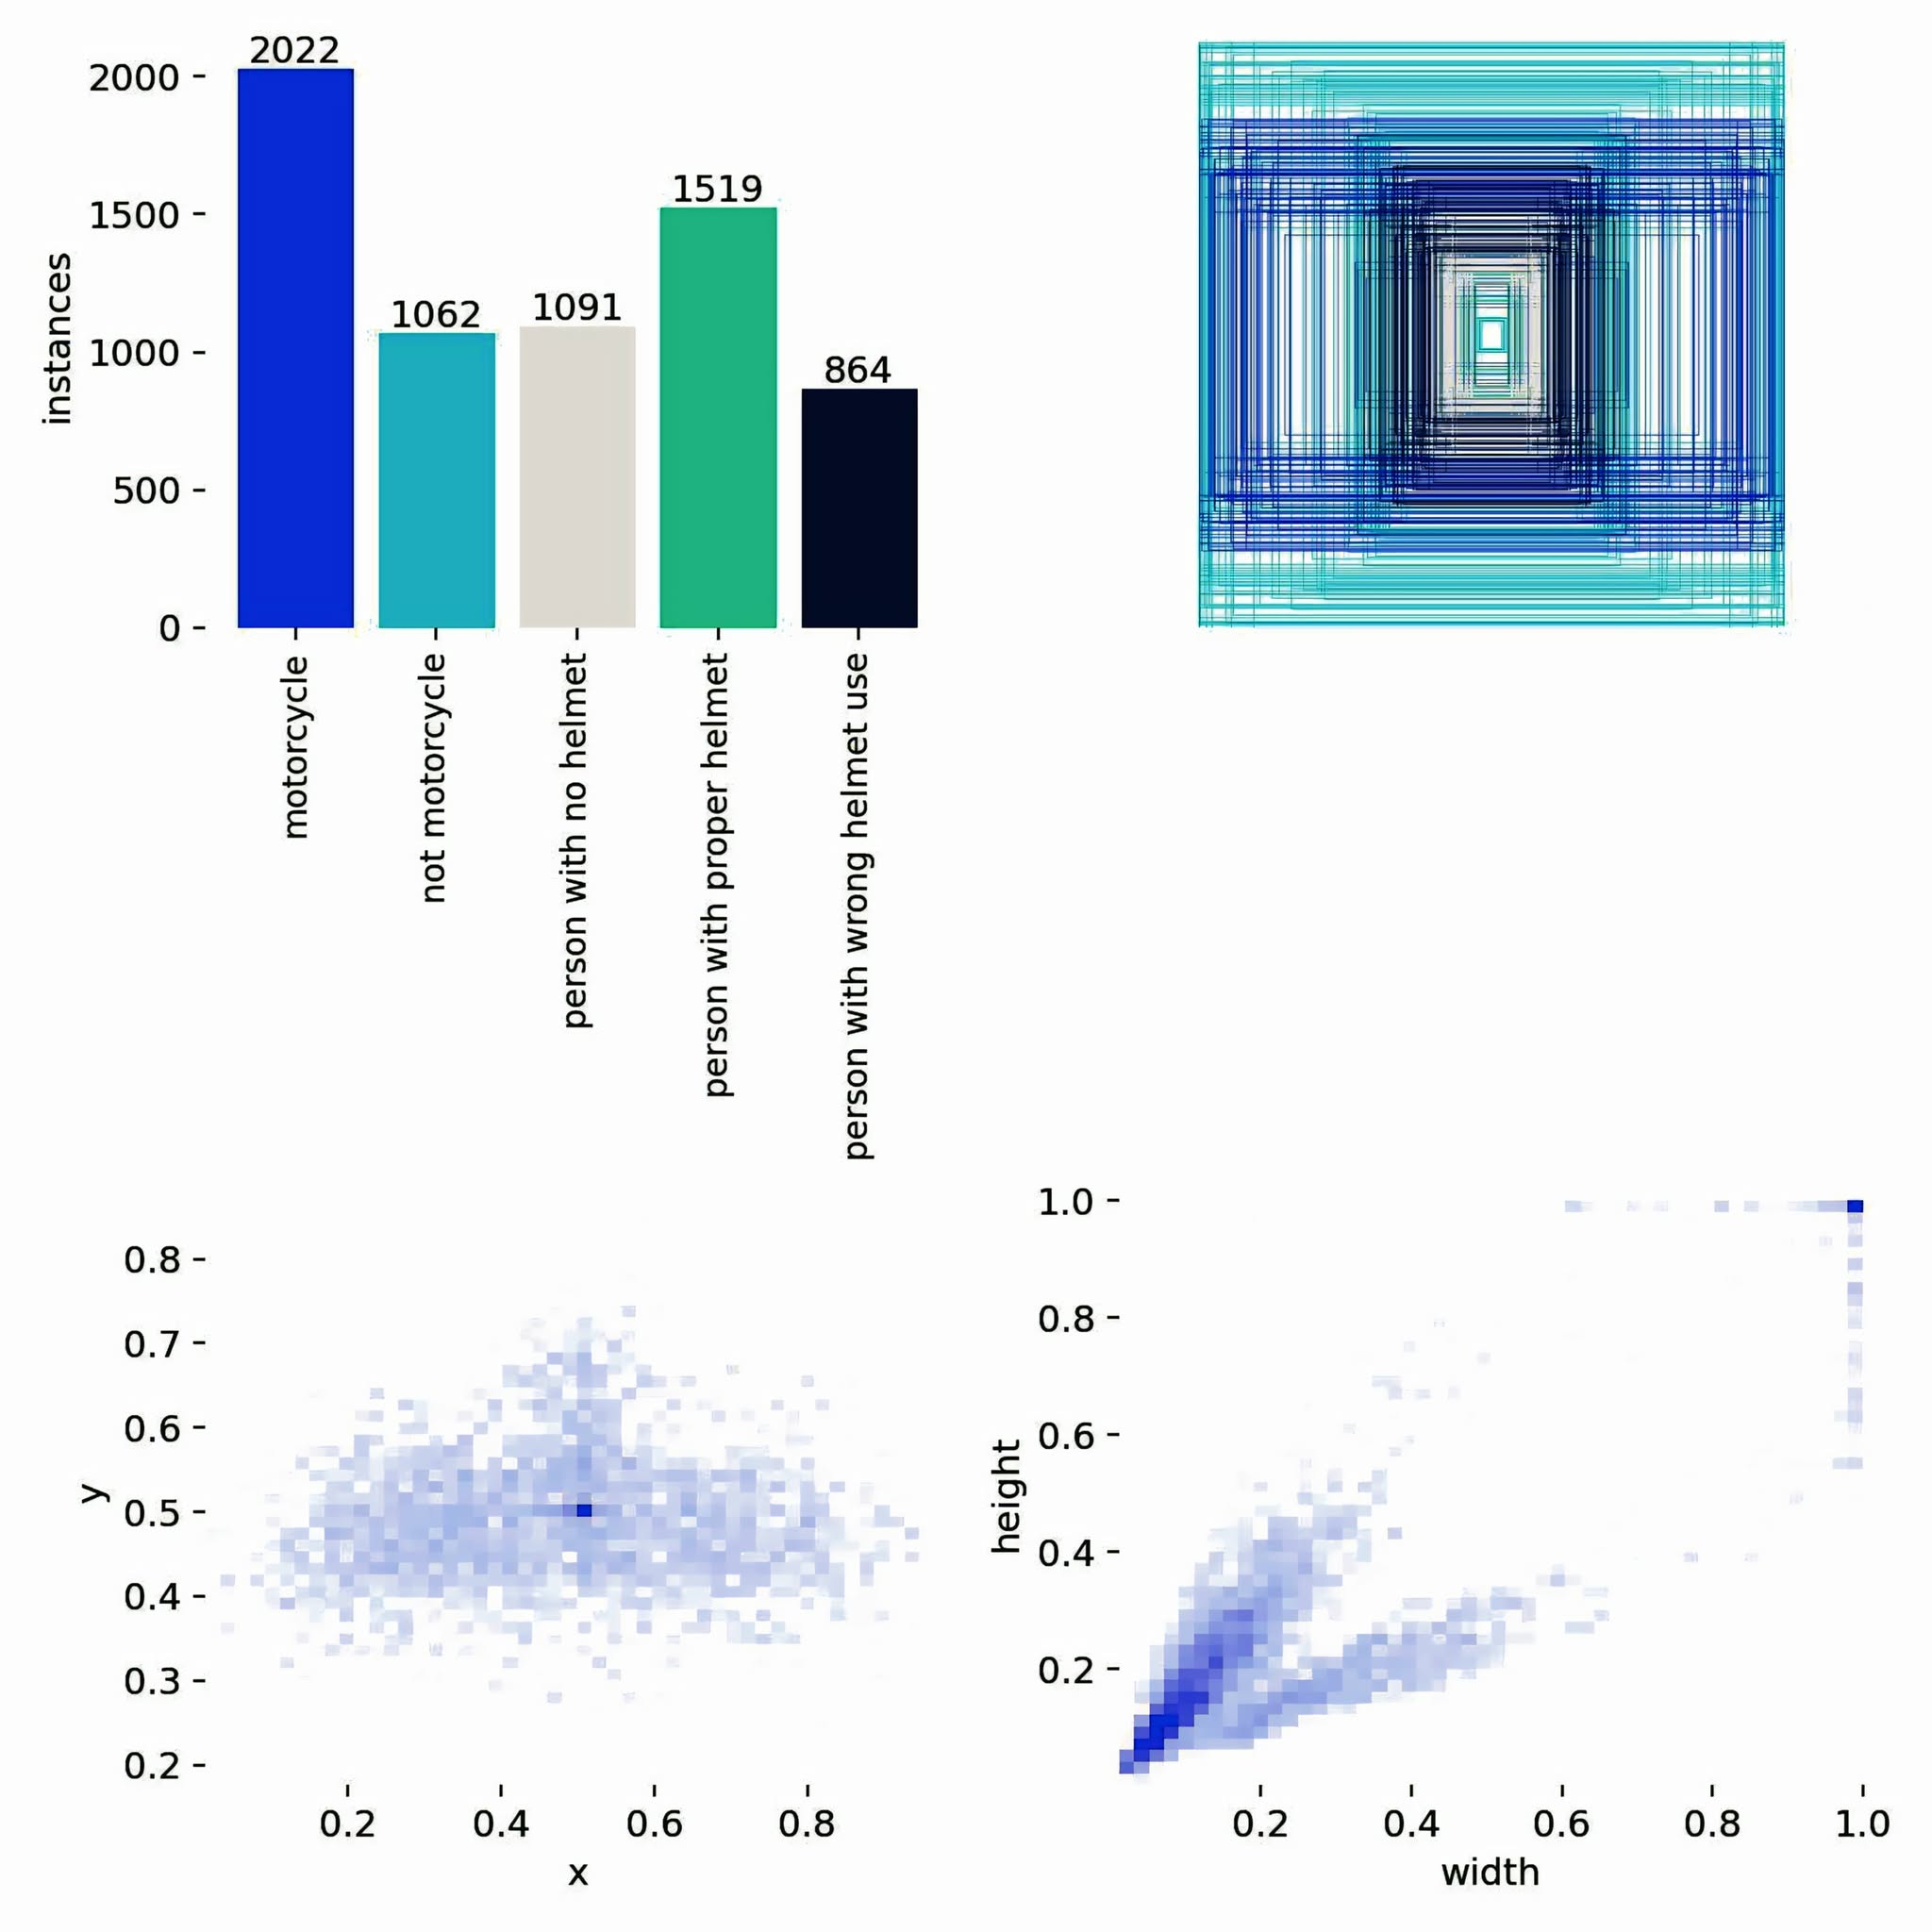
\includegraphics[width=0.85\textwidth]{figures/Fig 16.jpg}
	\caption[Confusion Matrix]{Confusion Matrix}
	\label{fig:confusion_matrix}
\end{figure}

\noindent
The confusion matrix shows that the model performs very well in identifying motorcycles (96\%) and non-motorcycles (98\%). However, it has moderate accuracy in detecting helmet-related classes, with 73\% for no helmet, 77\% for proper helmet, and 72\% for wrong helmet use. Misclassifications often occur between proper and wrong helmet use, or between no helmet and background. This means the model is strong in detecting motorcycles but still struggles with fine distinctions in helmet usage and separating persons from the background.

\subsubsection{Dataset Visualization}
\begin{figure}[ht]
    \centering
	\includegraphics[width=0.85\textwidth]{figures/Fig 17.jpg}
	\caption[Dataset Visualization]{Dataset Visualization}
	\label{fig:dataset_visualization}
\end{figure}

\noindent
The dataset visualization highlights the distribution and positioning of the annotated classes. The bar chart shows that motorcycles (2022 instances) and persons with proper helmet use (1519 instances) dominate the dataset, while wrong helmet use (864 instances) is the least represented, indicating some class imbalance. Persons without helmets (1062) and non-motorcycle objects (1091) also contribute significantly to the dataset. The bounding box heatmap suggests that most objects are centered in the images, which may help the model focus on relevant regions. Additionally, the width and height distribution indicates that many objects are relatively small, with fewer larger ones, which may influence detection accuracy. Overall, the dataset provides a strong foundation for training but requires attention to class imbalance to ensure balanced performance across all categories.

\subsubsection{Box Curve}
\begin{figure}[H]
\centering
\begin{tabular}{cc}
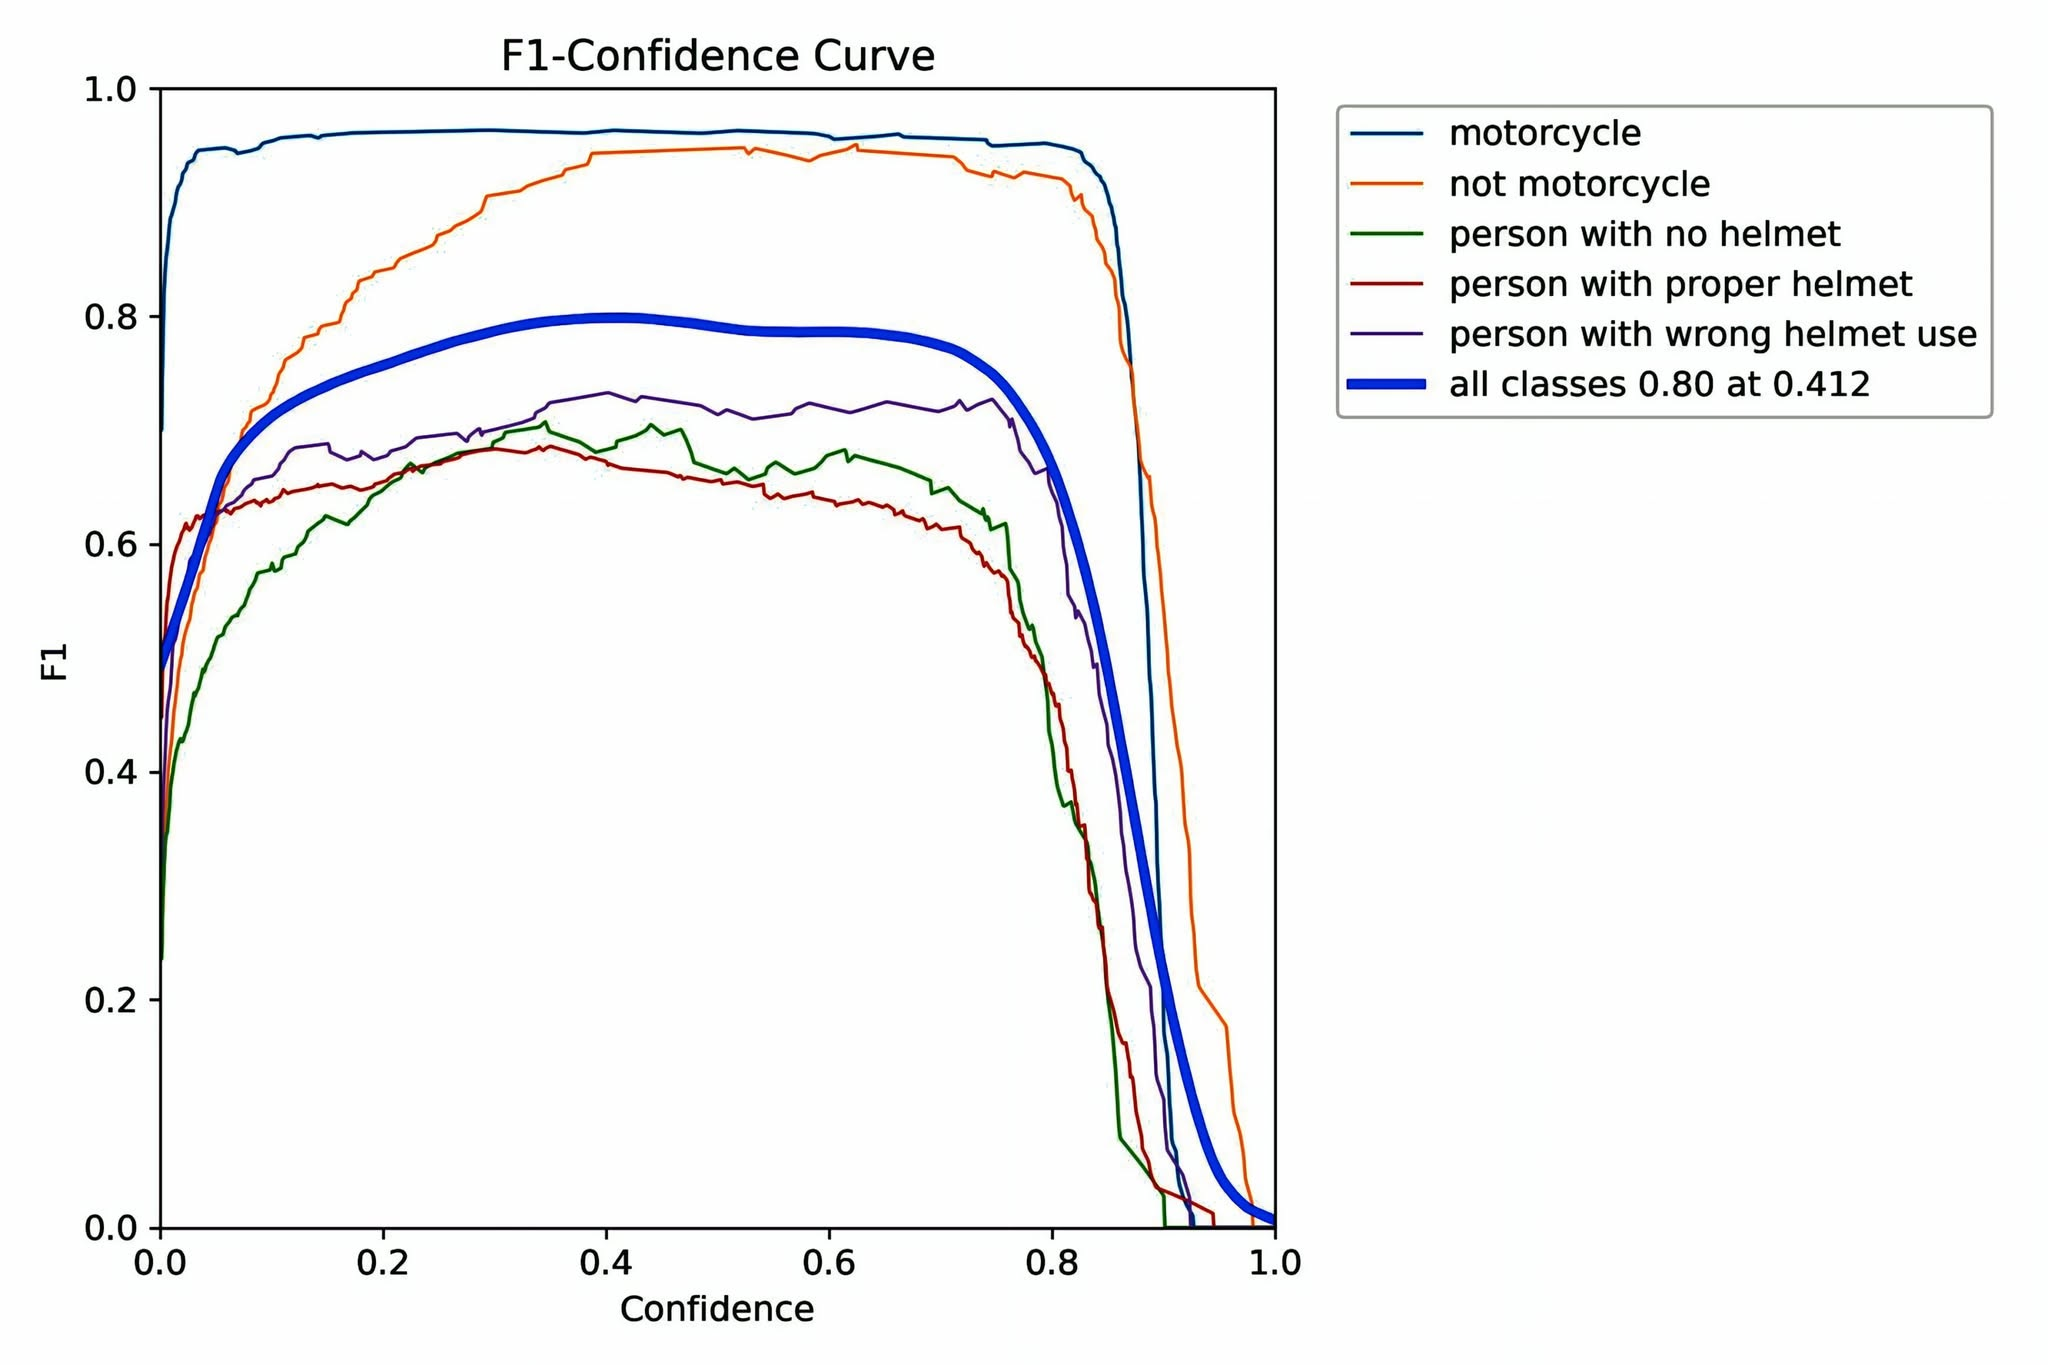
\includegraphics[width=0.45\textwidth]{figures/Fig18a.jpg} &
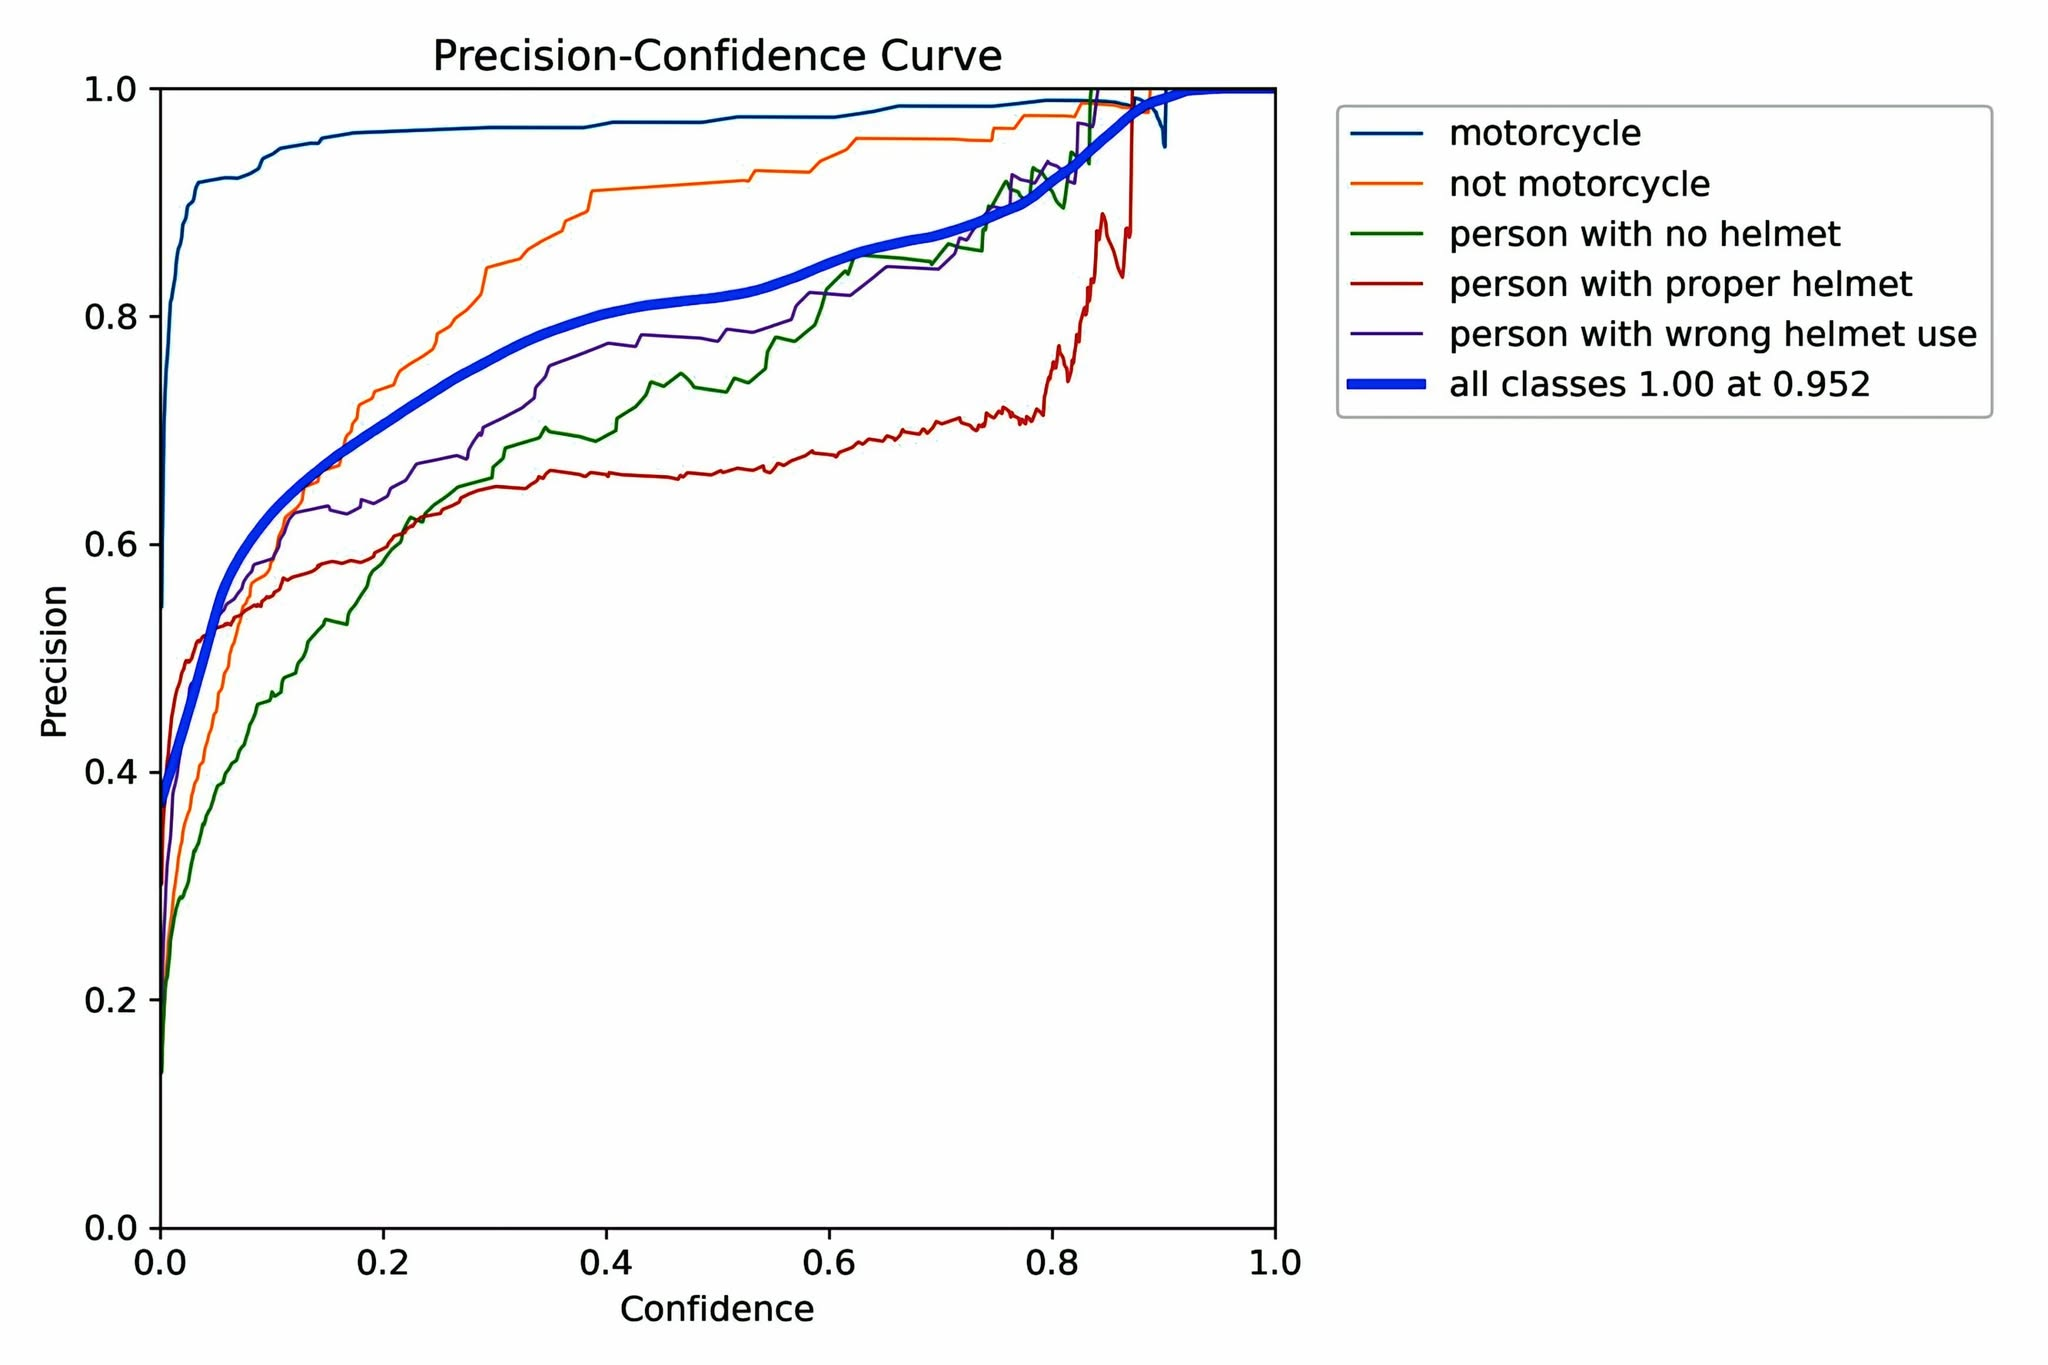
\includegraphics[width=0.45\textwidth]{figures/Fig18b.jpg} \\
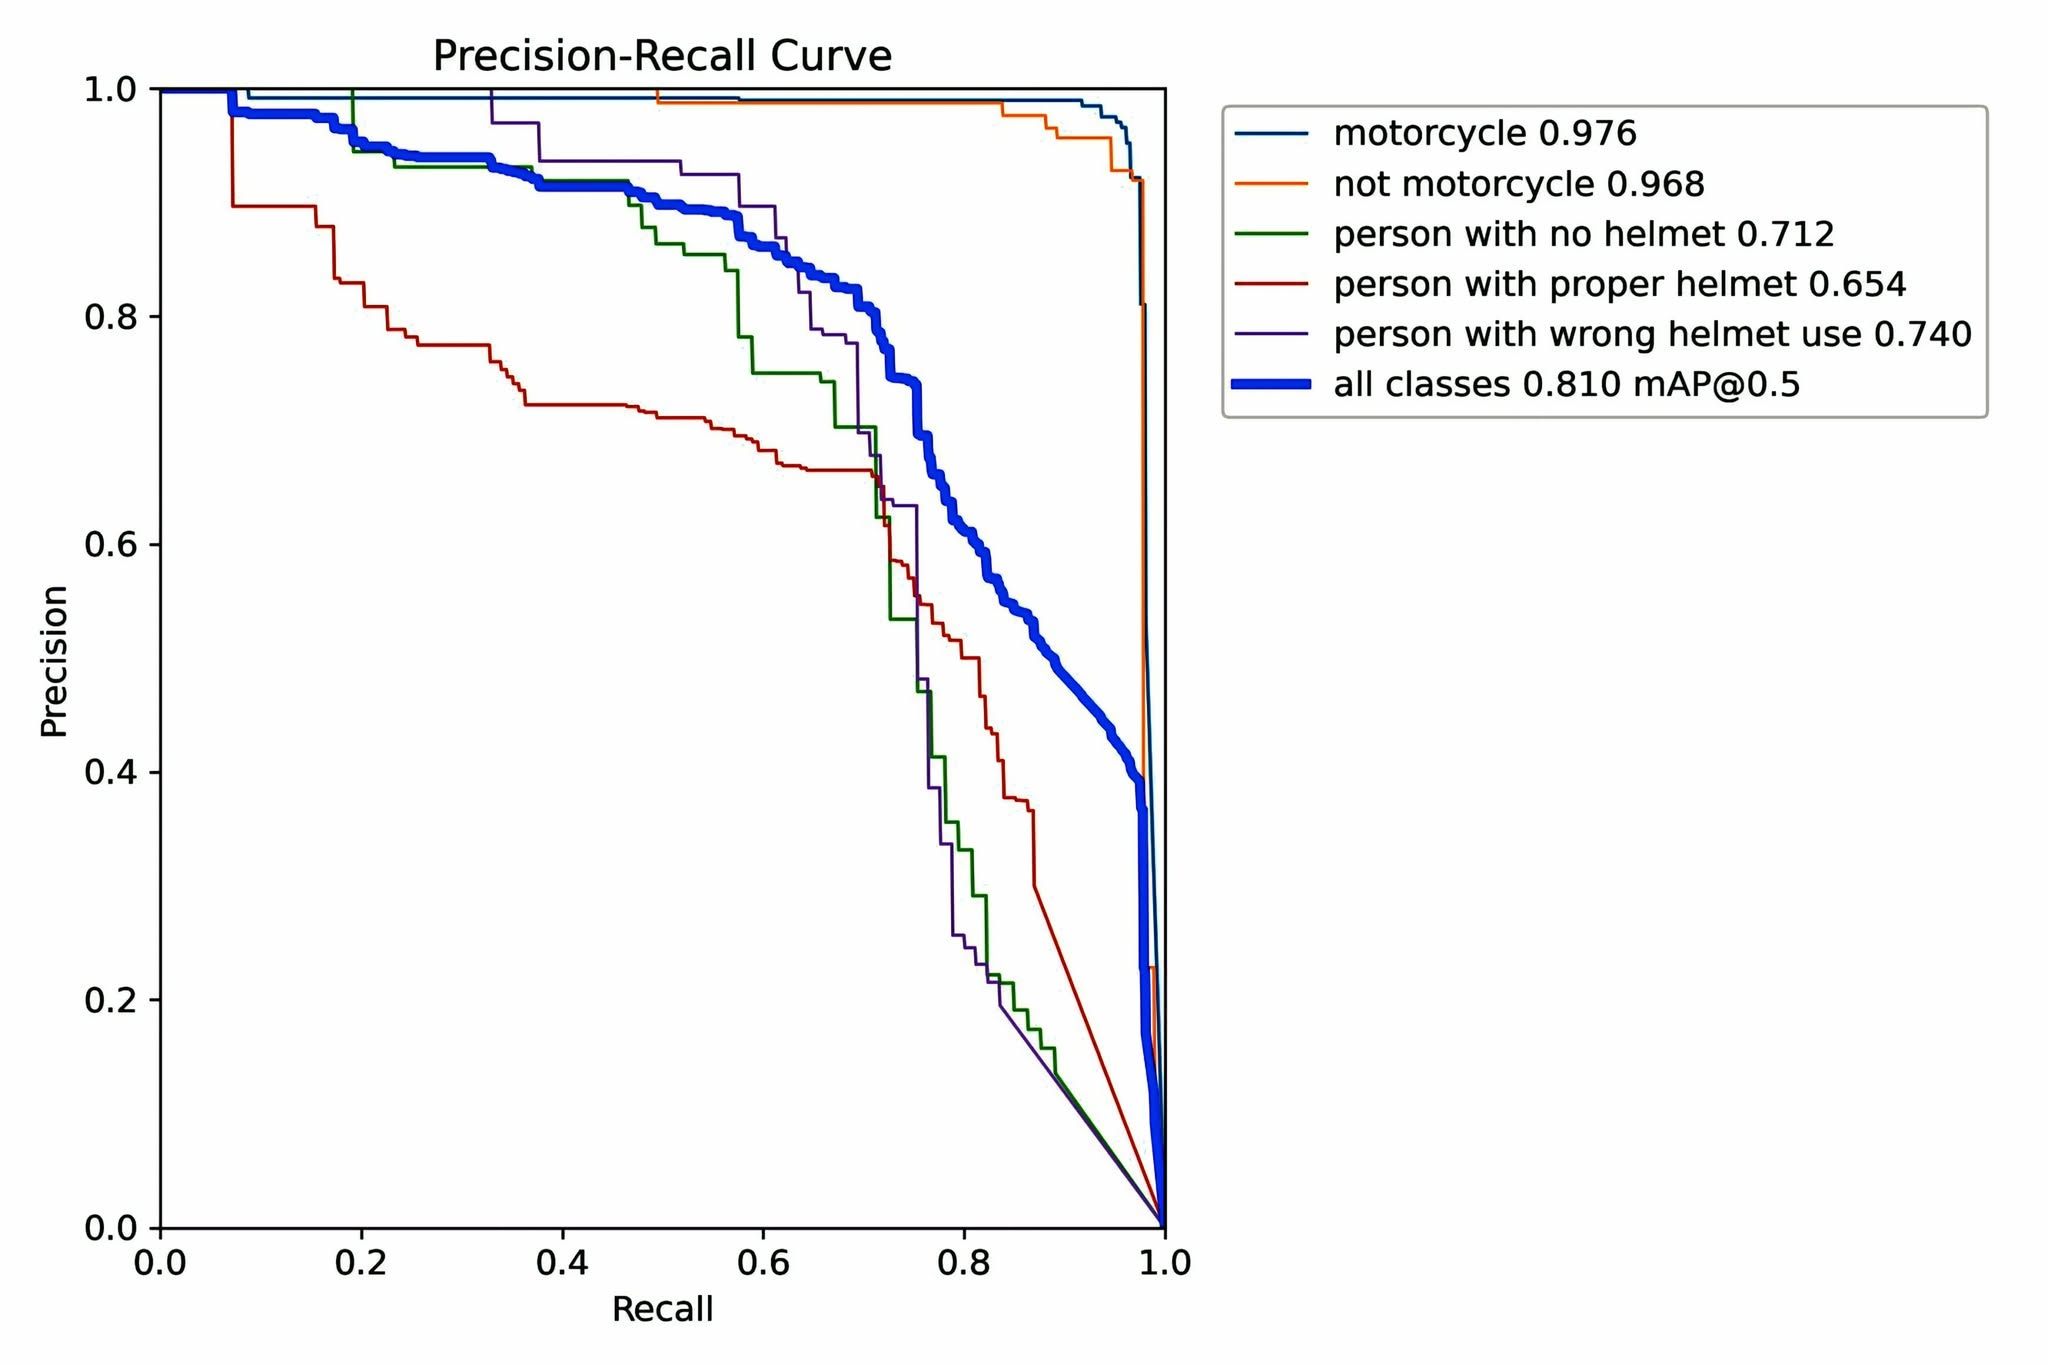
\includegraphics[width=0.45\textwidth]{figures/Fig18c.jpg} &
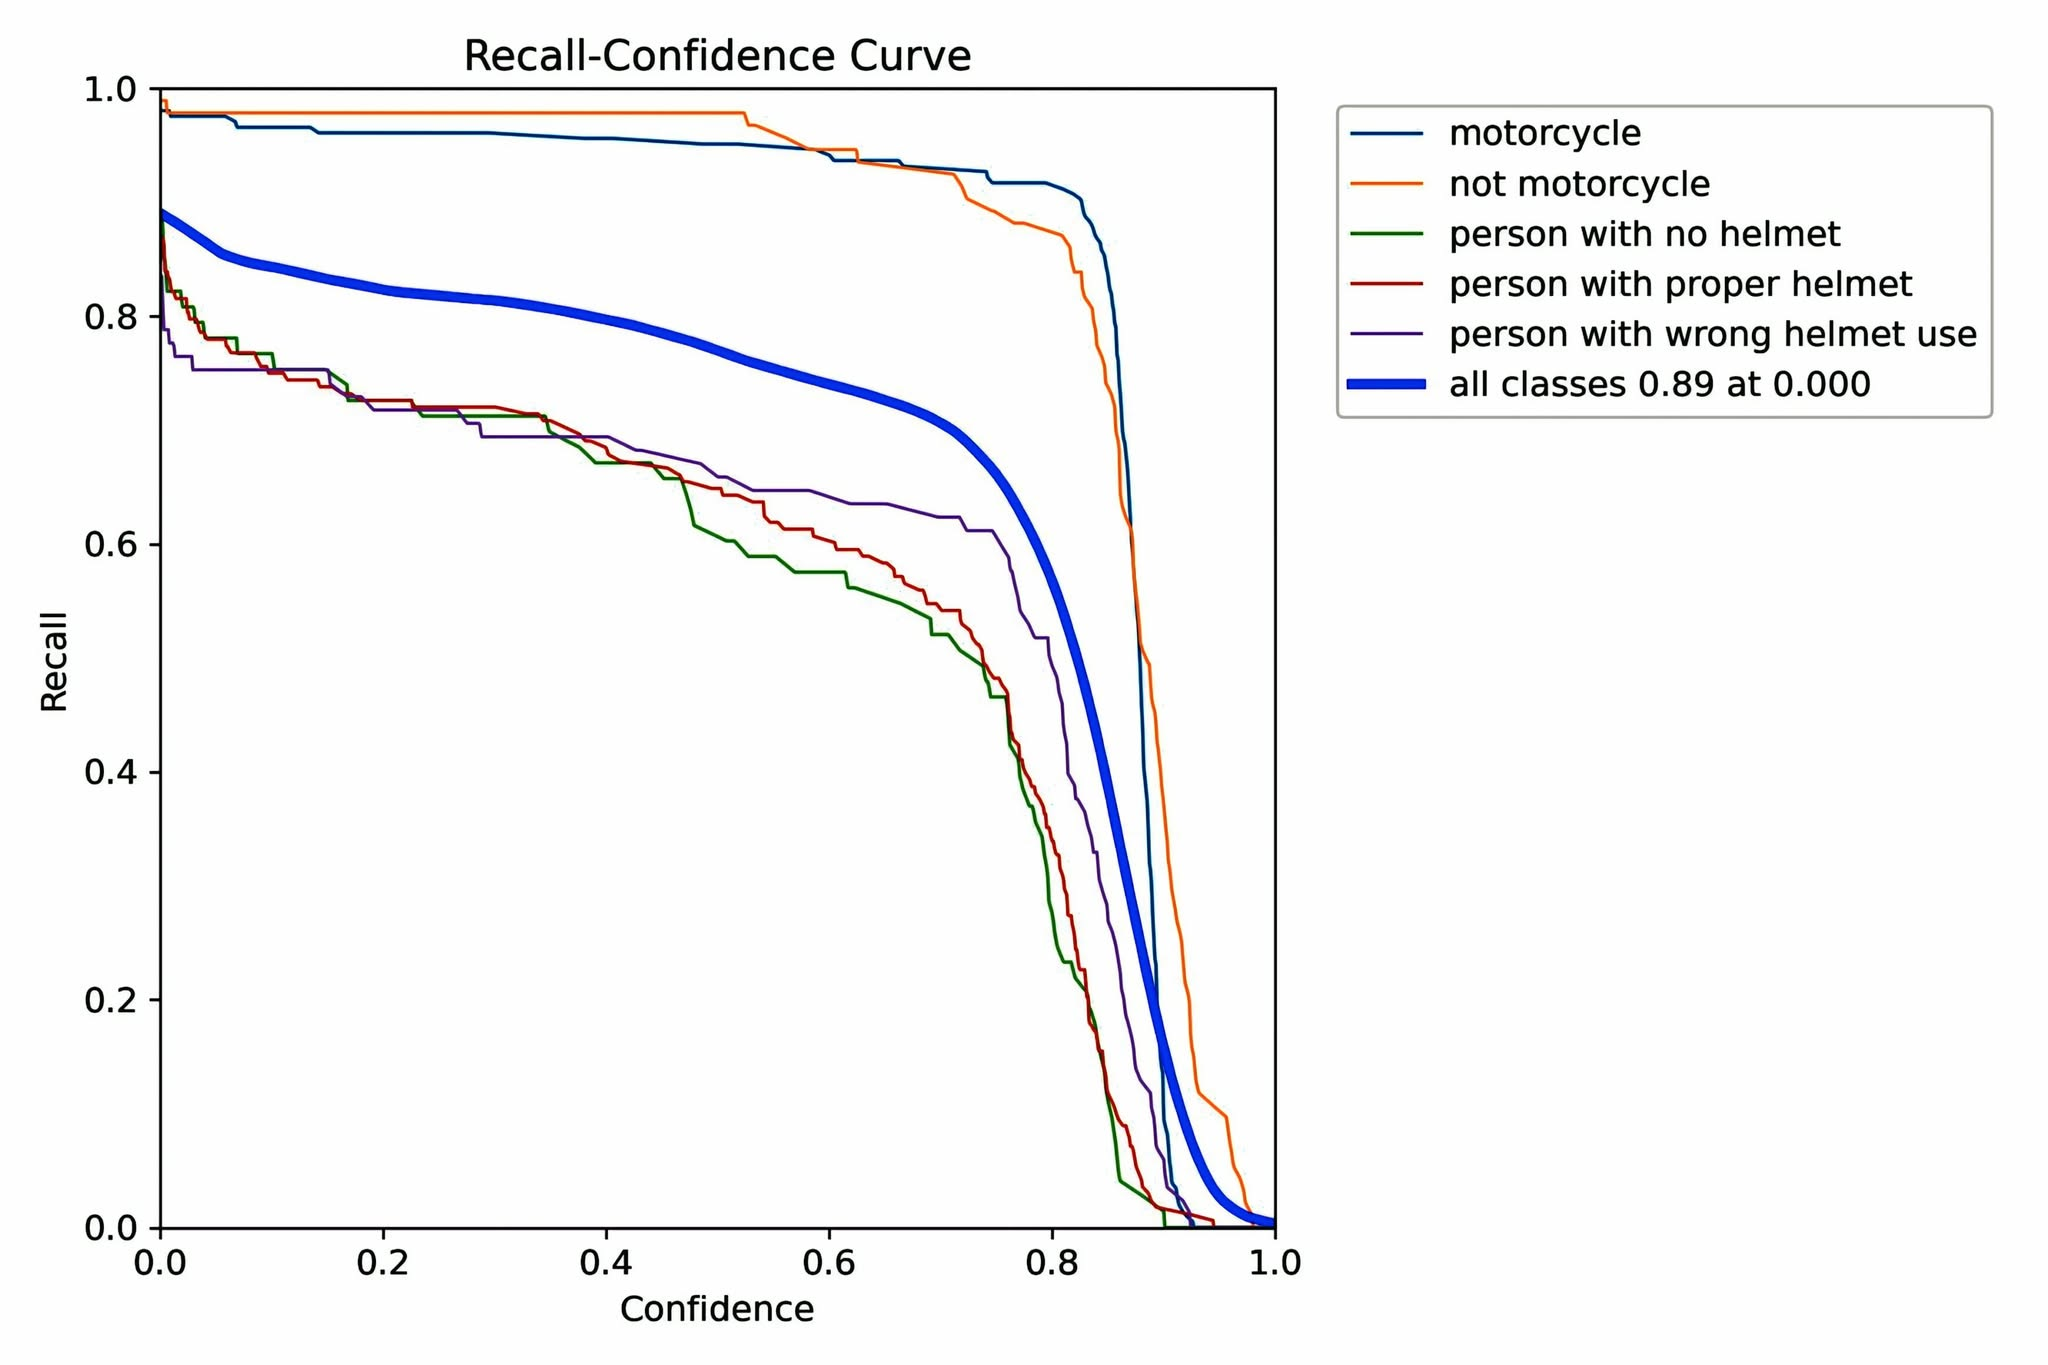
\includegraphics[width=0.45\textwidth]{figures/Fig18d.jpg} \\
\end{tabular}
\caption{Box Curve Results}
\label{fig:box_curve}
\end{figure}

\noindent
The performance evaluation graphs provide insights into how well the model detects motorcycles and helmet usage. In the F1-Confidence Curve (Graph A), the model achieves its best balance between precision and recall at a confidence threshold of around 0.41, with an overall F1 score of 0.80. The classes motorcycle and not motorcycle consistently achieve higher F1 scores compared to the helmet-related classes. The Precision-Confidence Curve (Graph B) shows that precision improves as the confidence threshold increases, with motorcycle and not motorcycle approaching near-perfect precision at high thresholds, while helmet-related classes such as proper helmet use and no helmet show lower precision values. The Precision-Recall Curve (Graph C) highlights that the model performs very well in detecting motorcycles (0.976) and non-motorcycles (0.968), but has lower average precision scores for helmet-related categories, with no helmet at 0.712, proper helmet use at 0.654, and wrong helmet use at 0.740, resulting in an overall mean Average Precision (mAP@0.5) of 0.810. Lastly, the Recall-Confidence Curve (Graph D) indicates that recall is highest at lower confidence thresholds, with an overall recall of 0.89, but gradually decreases as confidence increases, showing that while the model can detect most objects at low thresholds, higher thresholds ensure more reliable but fewer detections.

\begin{figure}[H]
\centering

% First row
\begin{minipage}{0.3\textwidth}
\centering
\textbf{Motorcycle} \\
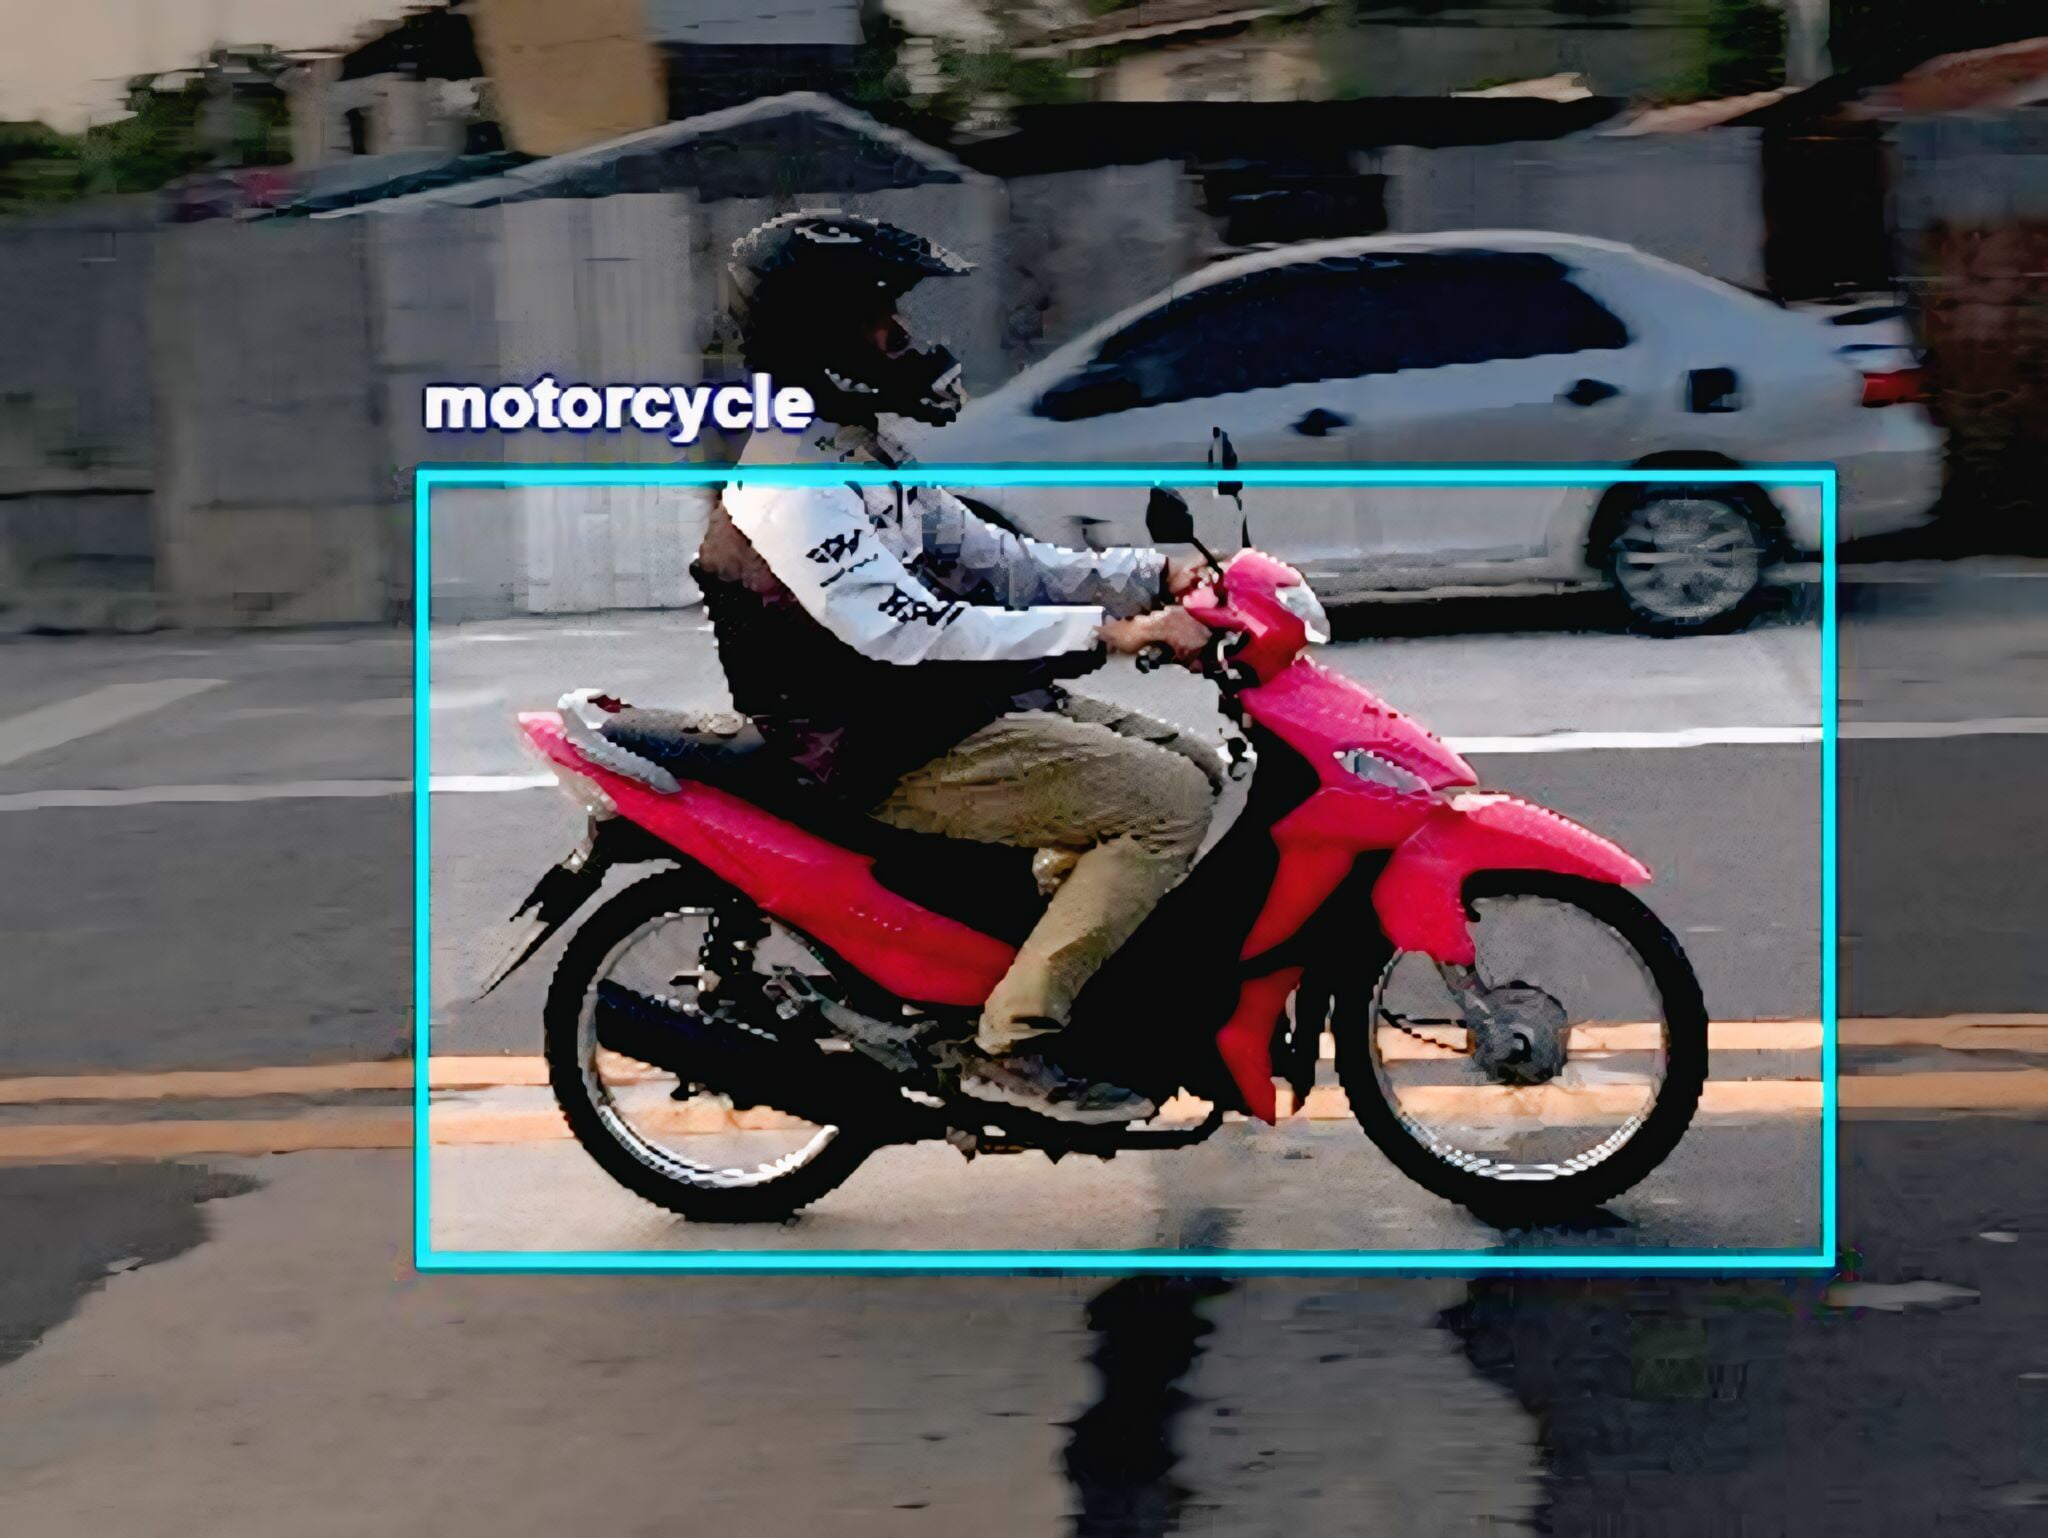
\includegraphics[width=\linewidth]{figures/Fig 19a.jpg}
\end{minipage}\hfill
\begin{minipage}{0.3\textwidth}
\centering
\textbf{Not motorcycle} \\
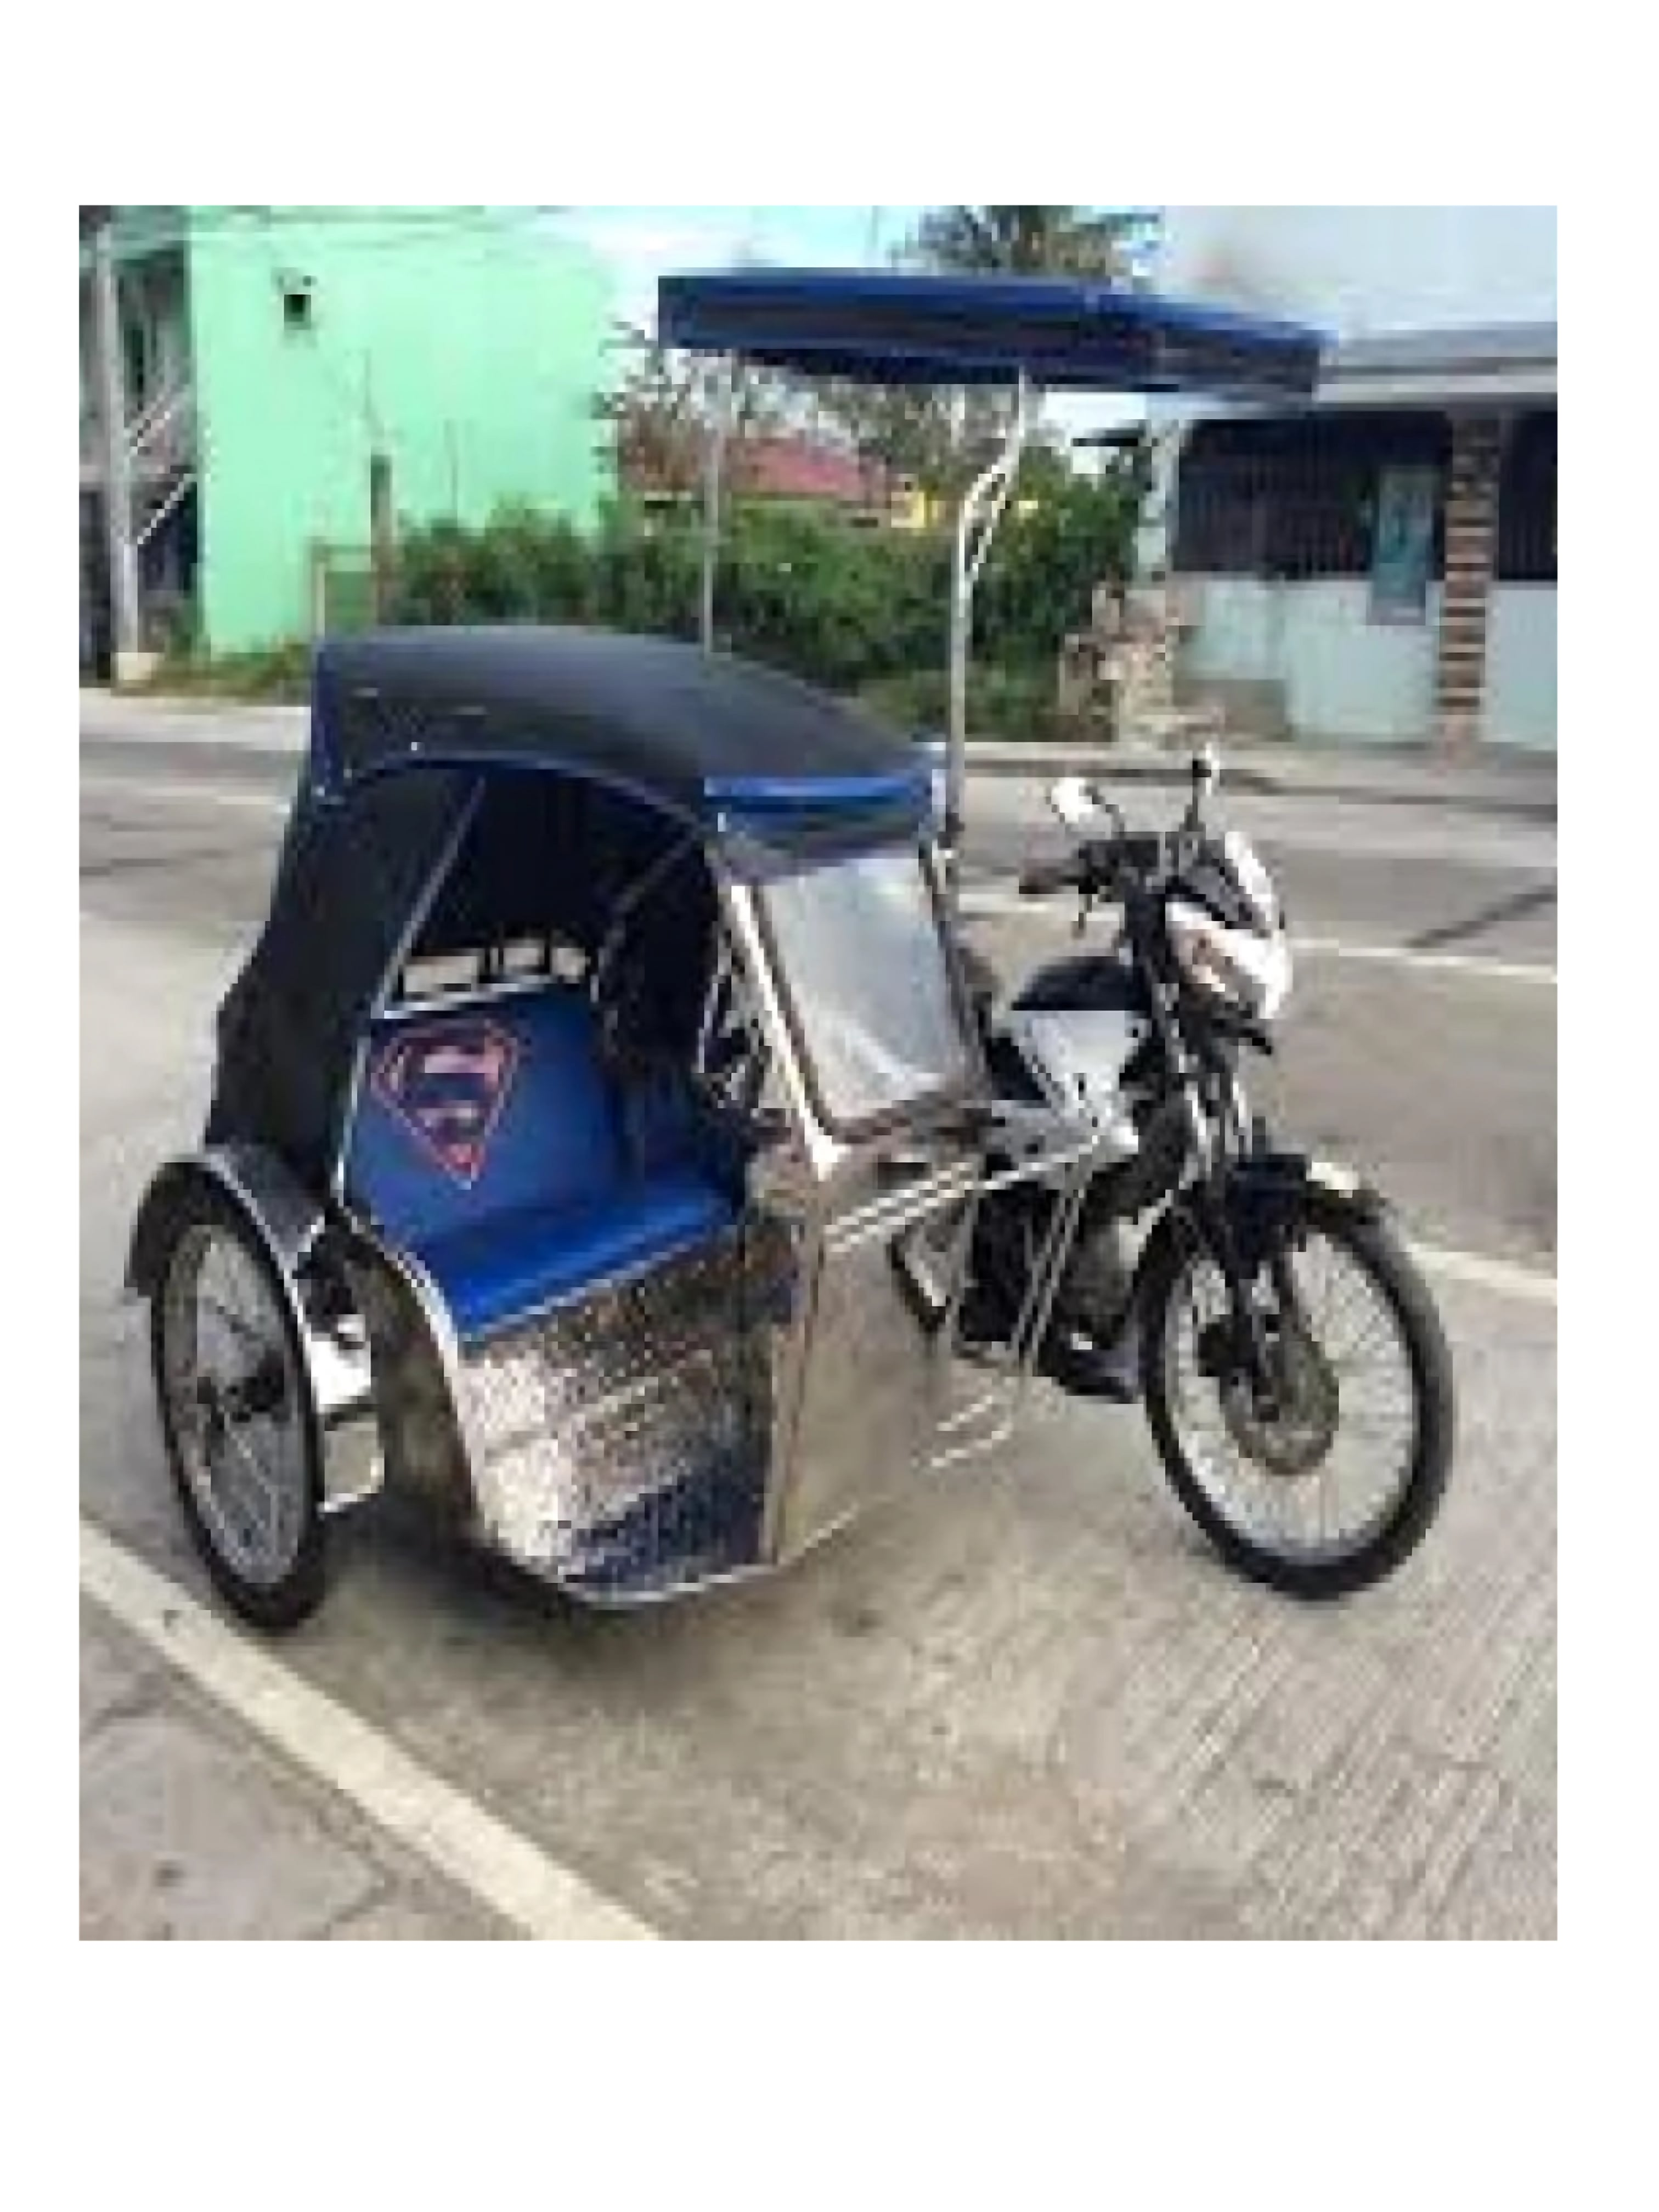
\includegraphics[width=\linewidth]{figures/Fig 19b.jpg}
\end{minipage}\hfill
\begin{minipage}{0.3\textwidth}
\centering
\textbf{Person with no helmet} \\
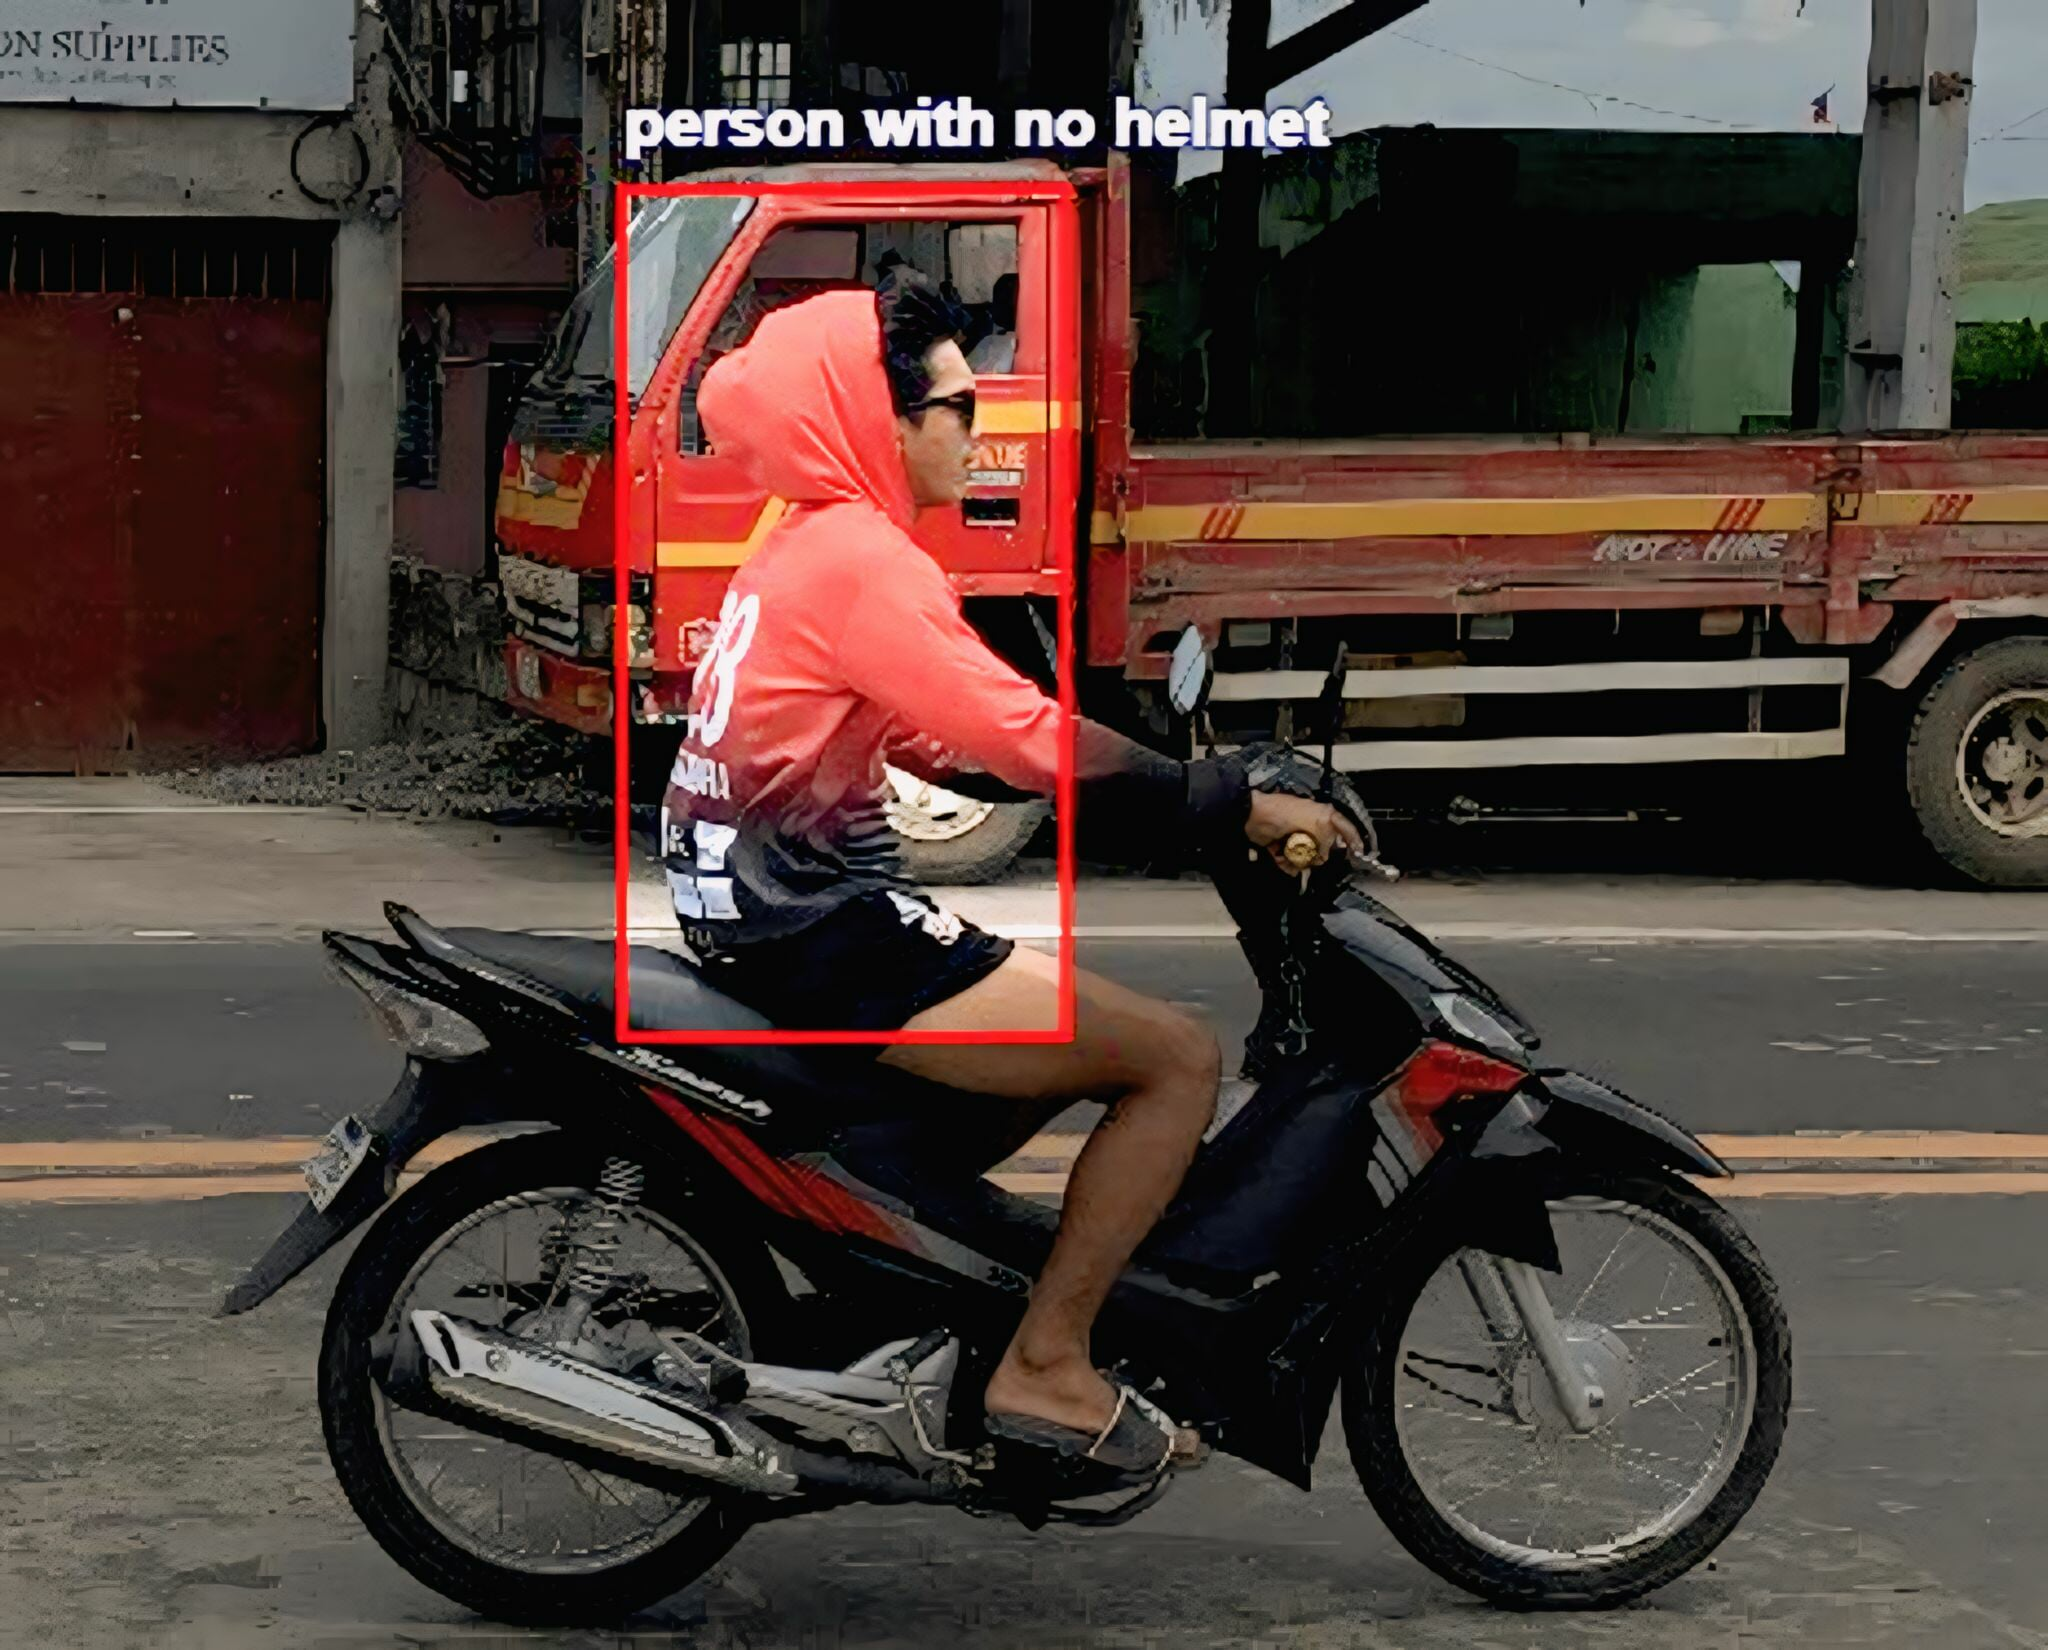
\includegraphics[width=\linewidth]{figures/Fig 19c.jpg}
\end{minipage}

\vspace{0.5cm}

% Second row
\begin{minipage}{0.45\textwidth}
\centering
\textbf{Person with proper helmet} \\
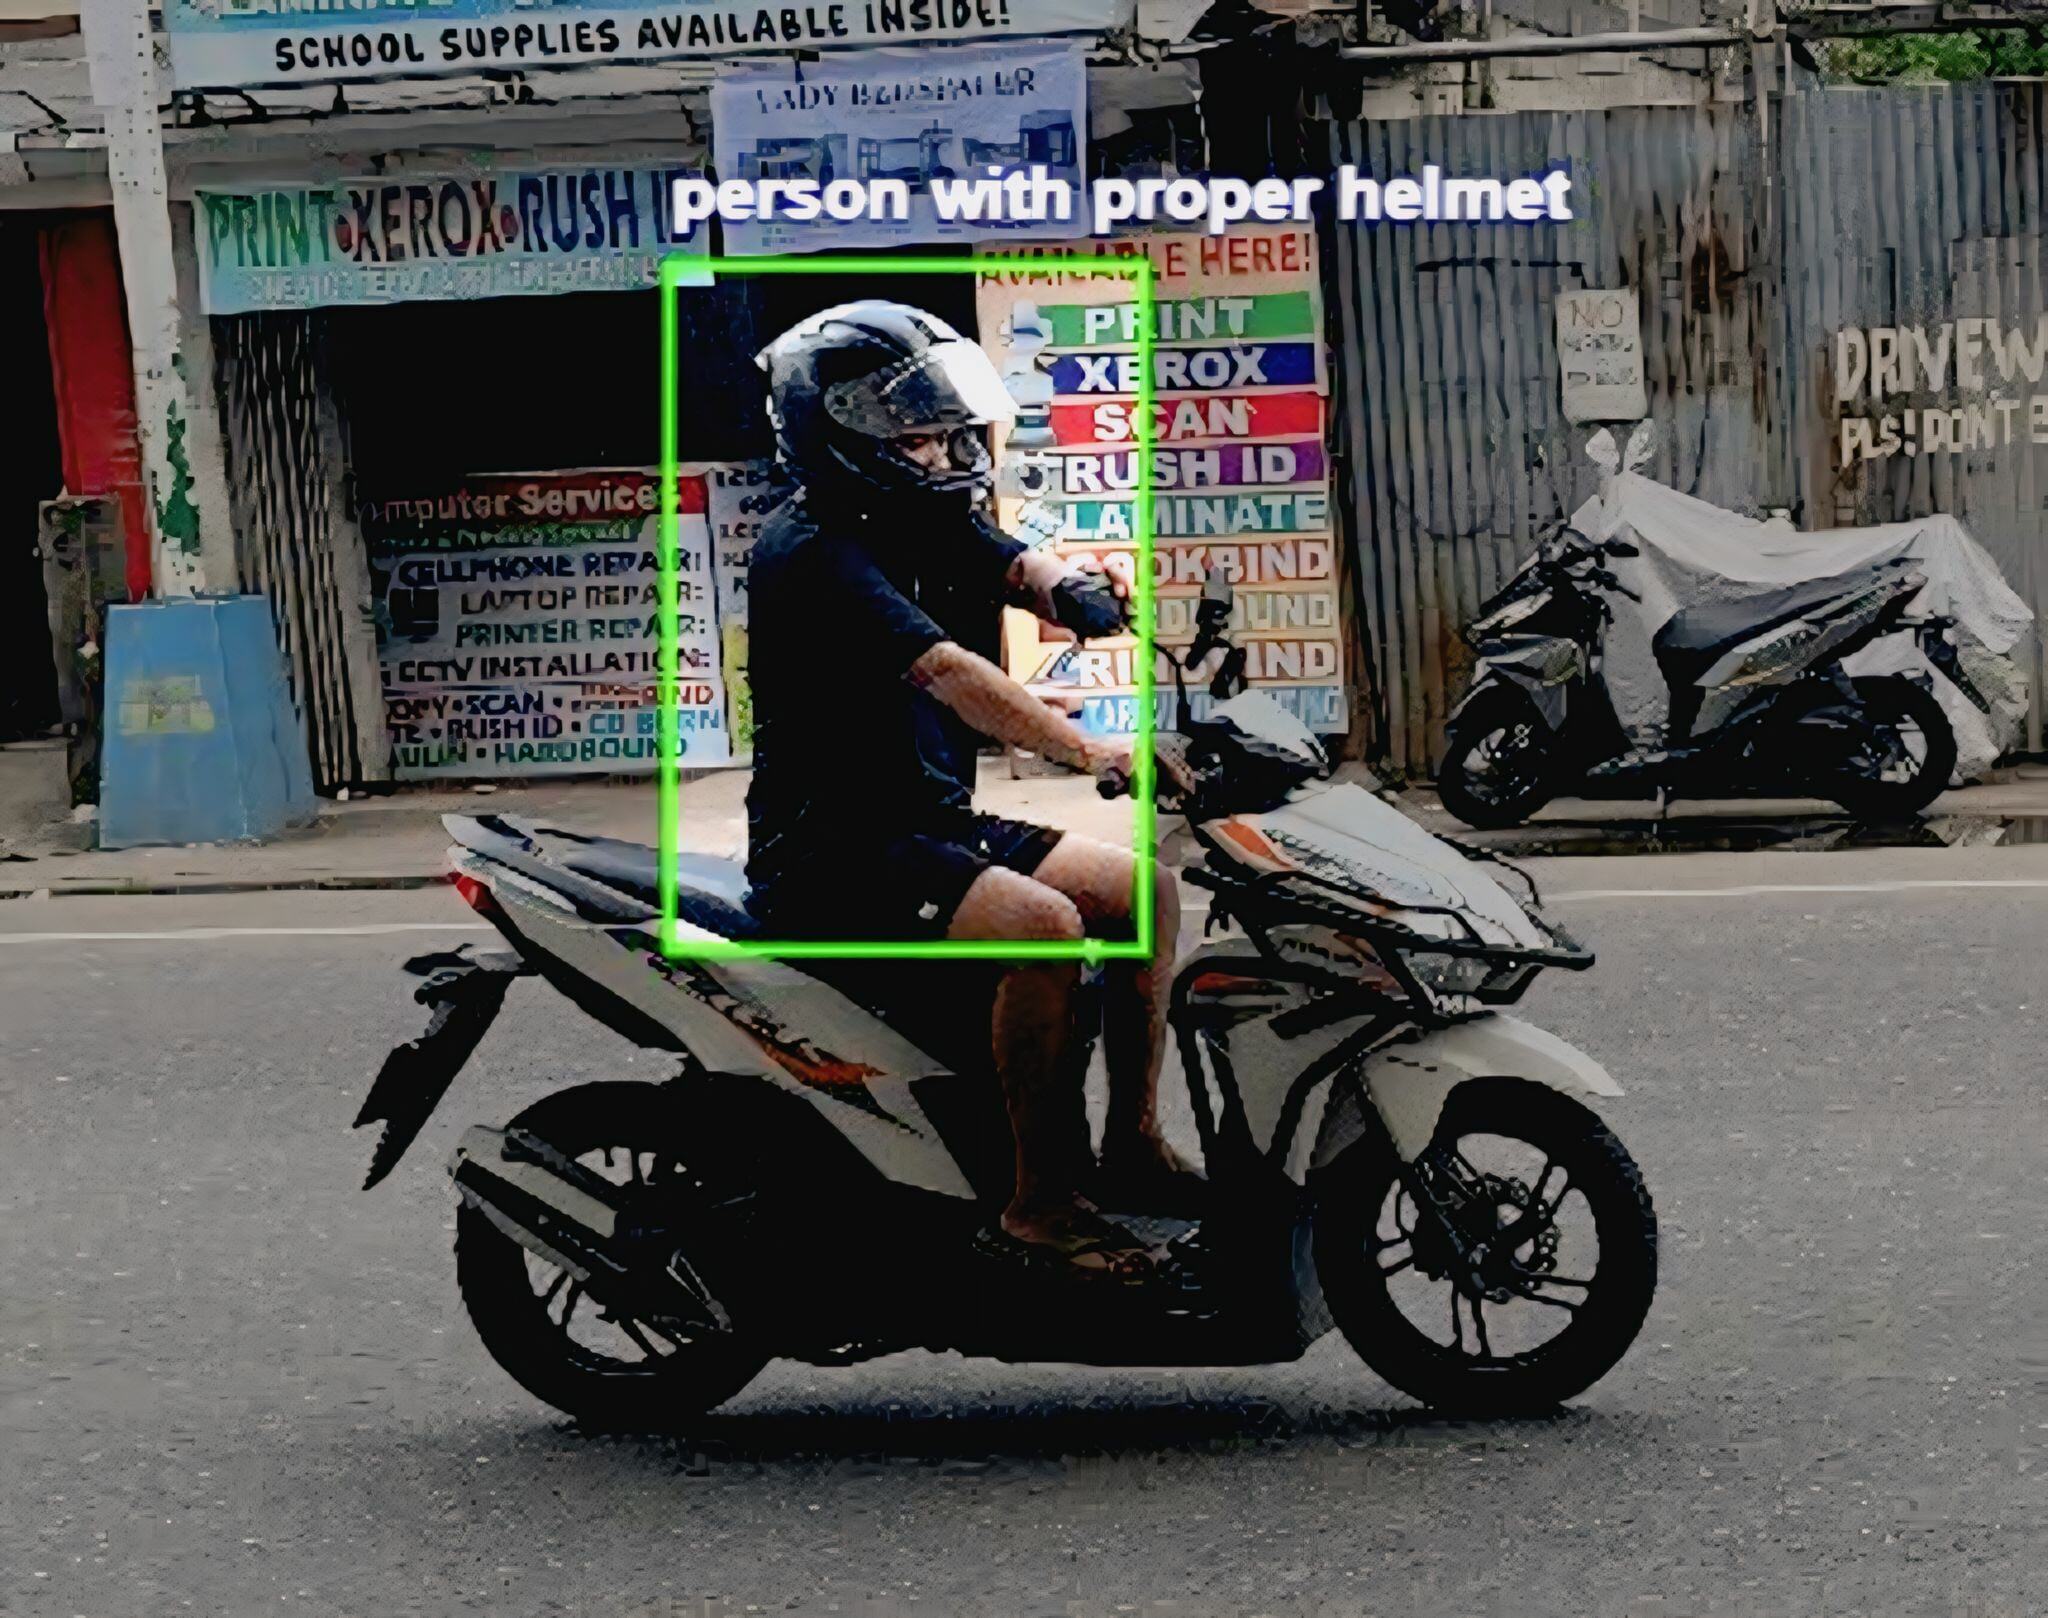
\includegraphics[width=\linewidth]{figures/Fig 19d.jpg}
\end{minipage}\hfill
\begin{minipage}{0.45\textwidth}
\centering
\textbf{Person with wrong helmet use} \\
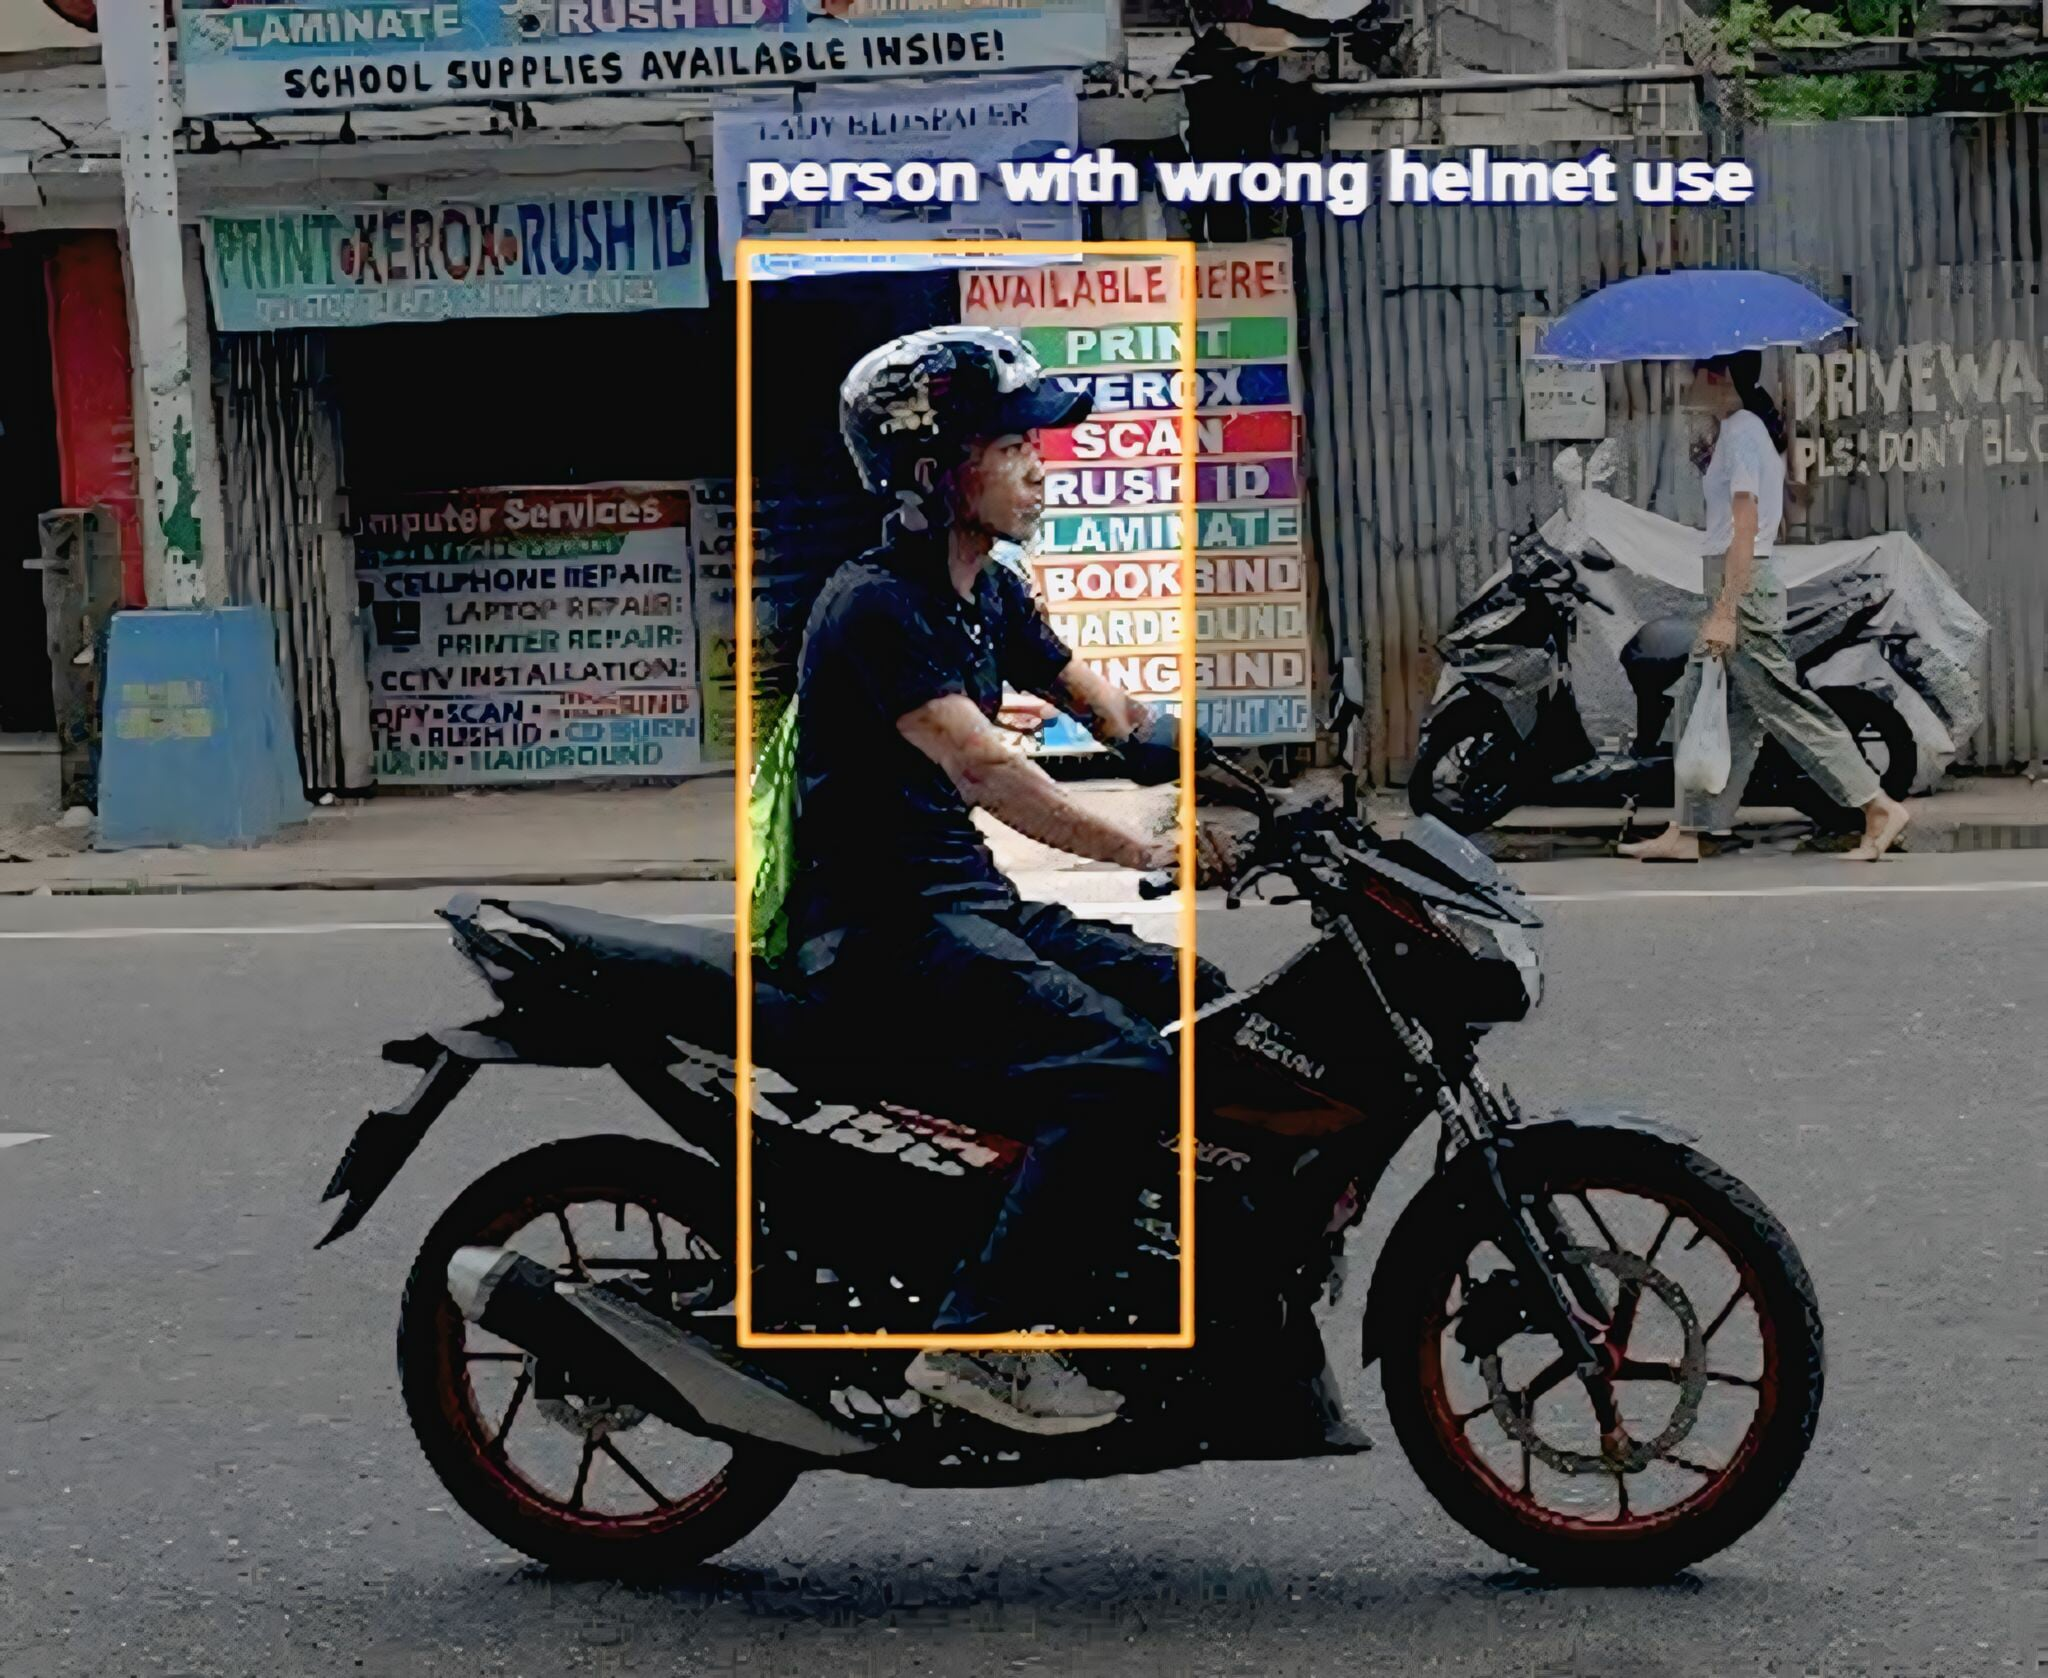
\includegraphics[width=\linewidth]{figures/Fig 19e.jpg}
\end{minipage}

\caption{Detection Results}
\label{fig:dataset_examples}
\end{figure}

\noindent
The results present sample outputs of the model using images from the validation set as well as real-time video captured through a webcam. Each output shows detected objects along with their predicted classes, including motorcycles, not motorcycles, persons with no helmet, persons with proper helmets, and persons with wrong helmet use. These outputs demonstrate how the model identifies helmet compliance in different scenarios, providing clear visual evidence of its performance. The prototype is integrated into a web-based interface, which allows users to view live detection results directly from the webcam feed. Frames are processed instantly by the model, enabling real-time monitoring of helmet usage and motorcycle presence. This setup highlights the model’s accuracy, detection capability, and practical applicability for continuous, real-time helmet compliance monitoring in various conditions.

\subsection{Vehicle Filtering}

Before detecting helmets, the prototype first identifies motorcycles in the camera feed. This is important because helmet detection only applies to motorcycles, not to bicycles, tricycles, e-bikes or other vehicles. The YOLOv8 model detects different types of vehicles, and only the motorcycles are selected for helmet detection. By filtering out non-motorcycle vehicles, the prototype reduces errors and ensures that helmet detection is faster and more accurate. This also allows the prototype to focus on relevant vehicles, which is important for real-time performance. 

\subsection{Helmet Detection}

\begin{figure}[ht]
    \centering
	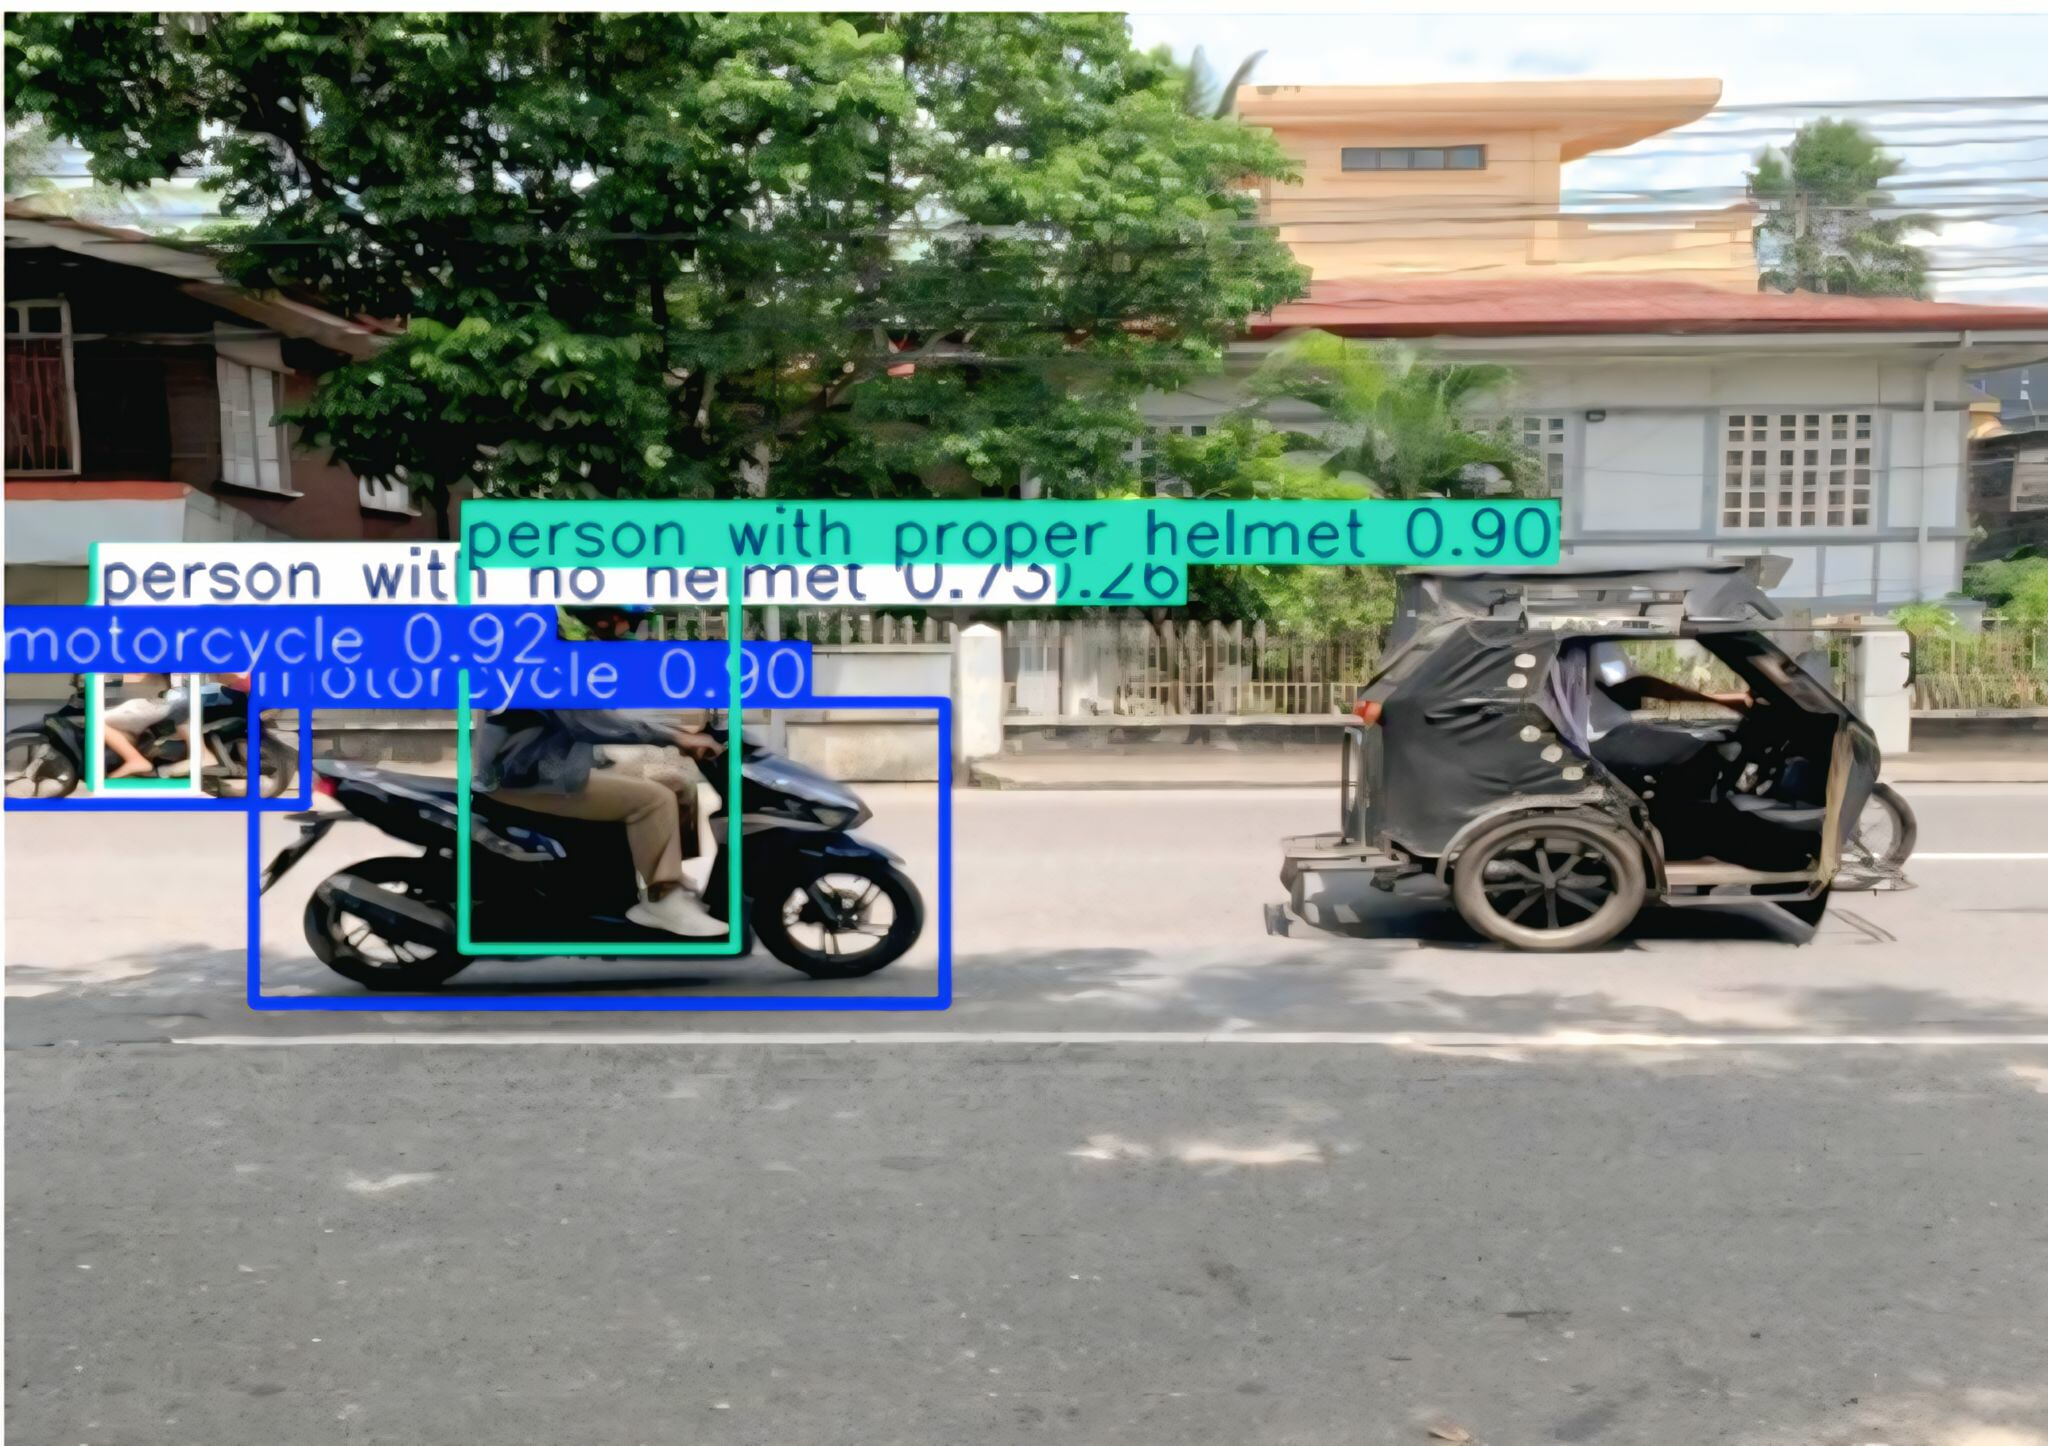
\includegraphics[width=0.85\textwidth]{figures/Fig 20.jpg}
	\caption[Helmet Detection]{Helmet Detection}
	\label{fig:helmet_detection}
\end{figure}

\noindent
After motorcycles are filtered from the camera feed, the prototype detects the helmet status of each rider. The YOLOv8 model was trained to classify riders into three categories: person with no helmet, person with proper helmet, and person with wrong helmet use.


By focusing only on motorcycles, the prototype reduces false detections and ensures accurate helmet compliance monitoring. The model processes the video feed in real-time, highlighting each rider and indicating their helmet status. Violations, such as riders without helmets or wearing them incorrectly, can be logged or trigger alerts, enabling timely monitoring and reporting of non-compliance.

\subsection{Real Time Monitoring}

The prototype performs helmet detection on motorcycles in real-time by processing live camera feeds. After vehicle filtering, each rider is classified as person with proper helmet, person with wrong helmet use, or person with no helmet. Violations are immediately highlighted, logged, or trigger alerts, enabling timely and accurate monitoring. This real-time processing ensures the prototype can be effectively deployed for on-road helmet compliance enforcement.

\subsection{Real Time Violation Alert}

\begin{figure}[ht]
    \centering
	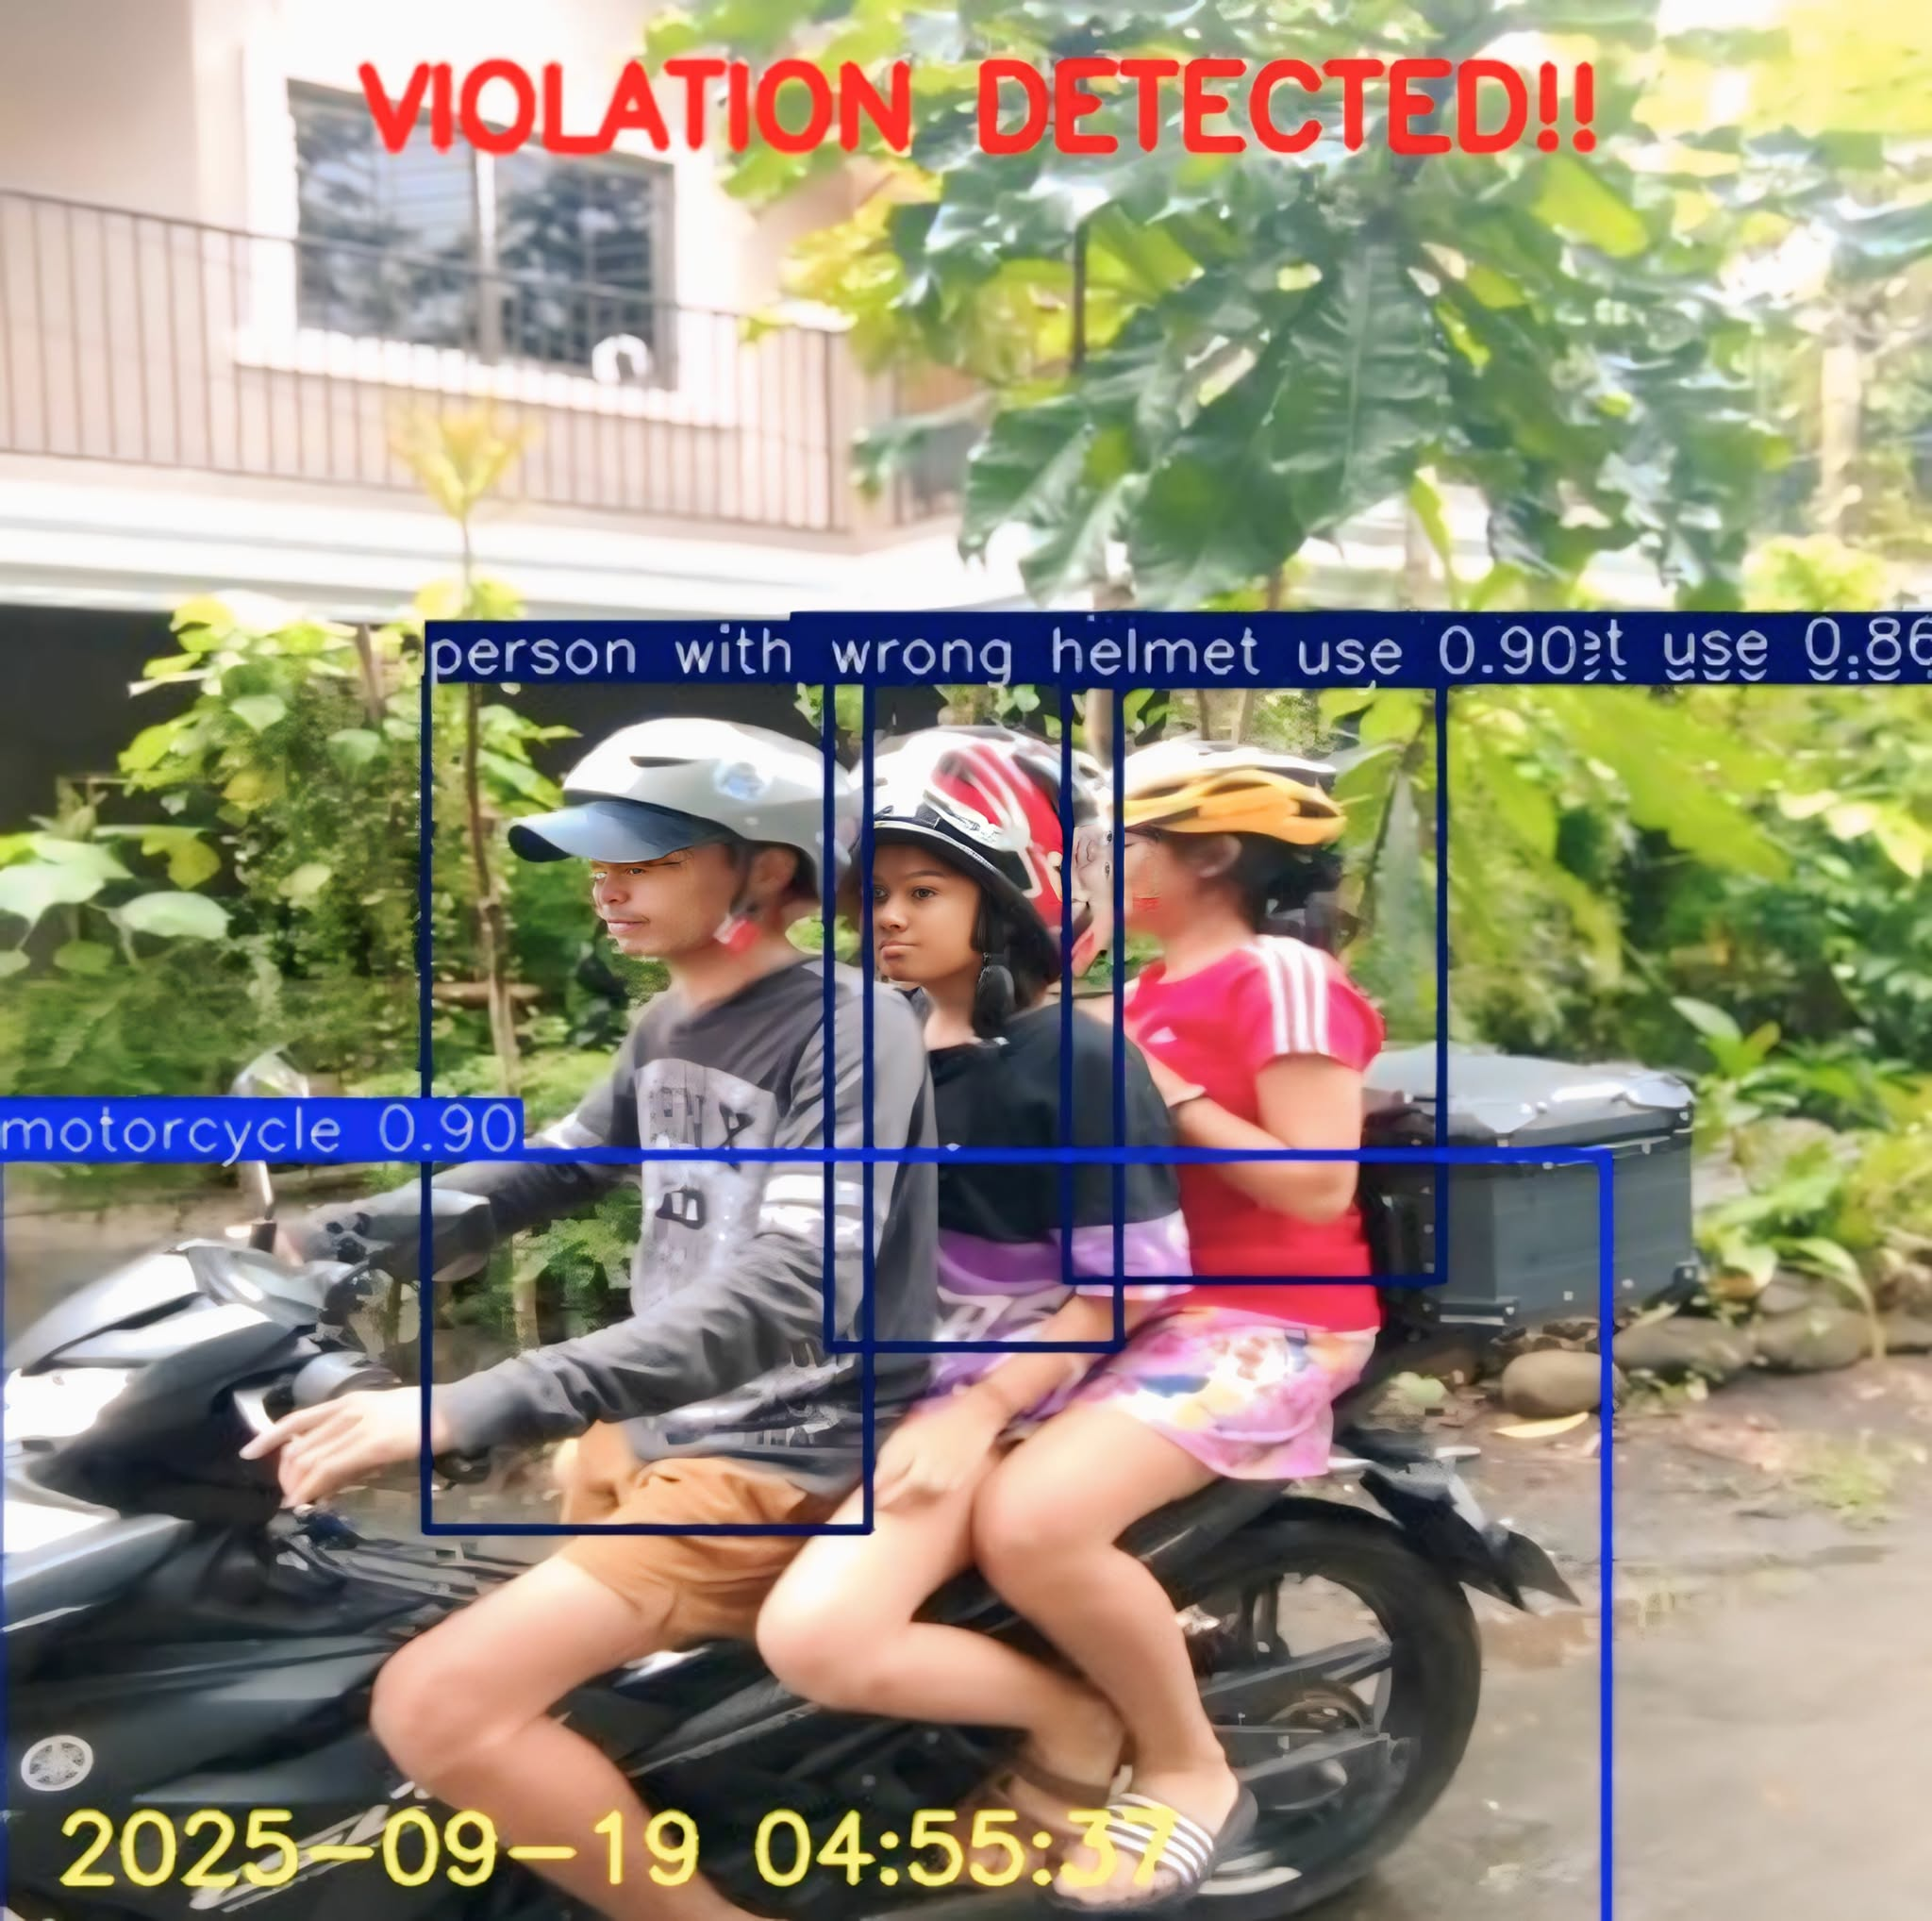
\includegraphics[width=0.85\textwidth]{figures/Fig 21.jpg}
	\caption[Real Time Violation Alert]{Real Time Violation Alert}
	\label{fig:real_time_violation_alert}
\end{figure}

\noindent
The prototype provides immediate alerts whenever a helmet violation is detected. When a rider is identified as not wearing a helmet or wearing it incorrectly, a red warning alert appears on the monitor displaying “Violation Detected.” At the same time, the prototype  automatically saves a video clip of the violation for documentation and reporting purposes. This feature ensures timely detection, accurate recording of violations, and supports effective enforcement of helmet compliance.







%=======================================================%
%%%%% Do not delete this part %%%%%%
\clearpage

\printbibliography[heading=subbibintoc, title={\texorpdfstring{\centering}{} Notes}]
\end{refsection}

    
\chapter{Conclusion}
\begin{refsection}
% text of this chapter goes here


\begin{figure}[ht]
    \centering
	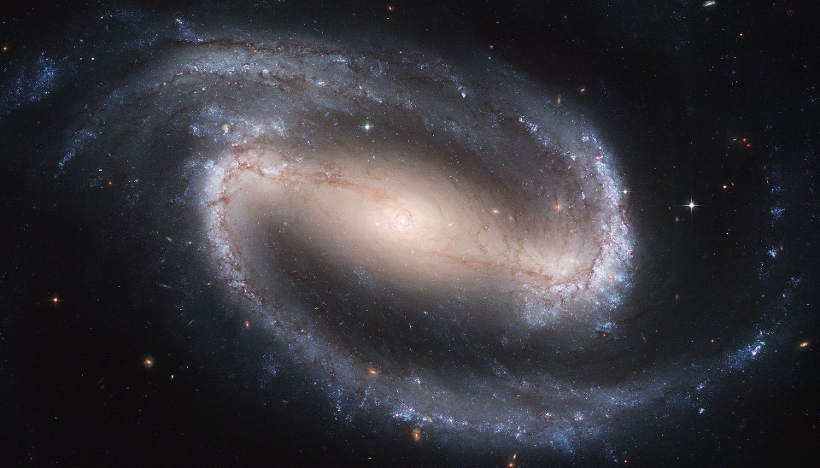
\includegraphics[width=0.85\textwidth]{figures/sampleFig1.jpg} 
	\caption[Barred spiral galaxy NGC 1300]{Barred spiral galaxy NGC 1300 photographed by Hubble telescope. While the galaxy in the photo is not our sun, it does emit light, much like our sun. Image credit: NASA.}
	\label{fig:firstFig}
\end{figure}


%=======================================================%
%%%%% Do not delete this part %%%%%%
\clearpage

\printbibliography[heading=subbibintoc, title={\texorpdfstring{\centering}{} Notes}]
\end{refsection}
    \makeBibliography
    
% The environment used here (theappendices) is a wrapper for the basic appendices environment which changes the appearance of the title page and the structure and appearance of the appendices in the table of contents and PDF bookmarks. The original functionality can be restored by simply removing the 'the' from the \begin{} and \end{} statements below.

\begin{theappendices}

\chapter{Language Editing Certification}
\centering

This is to certify that the undersigned has reviewed and went through all the pages of the Bachelor of Science in Computer Science thesis manuscript titled \\

\textbf{"ENTER YOUR TITLE HERE"} \\


of \textbf{AuthorName1}, \textbf{AuthorName2}, \textbf{AuthorName3}, as against the set of structural rules that govern research writing in accord with the composition of sentences, phrases, and words in the English language.
 \newline \newline \newline \\

\noindent \textbf{JUAN DE LA CRUZ} \\
\textit{Language Editor} \\

Date:\_\_\_\_\_\_\_\_\_\_\_\_\_\_\_\_\_\_\_\_\_\_\_


\chapter{Secretary's Certification}
\centering

This is to certify that the undersigned has provided accurate recommendations, suggestions, and comments unanimously agreed and approved by the panel of examiners during the oral examination of the thesis titled \\ \textbf{"ENTER YOUR TITLE HERE"} \\  prepared and submitted by \textbf{AuthorName1}, \textbf{AuthorName2}, \textbf{AuthorName3}, and that the same have not been amended, modified or obliterated. \newline \newline \newline \\



\textbf{MS. MARIA DAISY R. BELARDO} \\
\textit{Secretary} \\


Date:\_\_\_\_\_\_\_\_\_\_\_\_\_\_\_\_\_\_\_\_\_\_\_

\chapter{JOINT AFFIDAVIT OF UNDERTAKING (Plagiarism)}

\centering

\textbf{JOINT AFFIDAVIT OF UNDERTAKING}


% IN WITNESS WHEREOF, I have hereunto set my name this ____ day of ___________ 202__ in
% ___________________________________, Philippines.
% SUBSCRIBED AND SWORN TO before me this ___ day of ________ at _______________, Philippines,
% affiants exhibiting to me their competent proofs of identity above stated.
% Doc. No. ___________:
% Page No.: __________:
% Book No.: __________:
% Series of 202_.


\end{theappendices}
    % Vita should only be included for PhD candidates.

\begin{vita}

\begin{itemize}
    \item 
    
    \begin{figure}[ht]
        \centering
    	
\includegraphics[width=0.35\textwidth]{figures/person-icon.png}
    \end{figure}
    
    \textbf{Joseph Jessie S. Oñate} is a faculty member of the College of Computer Studies. He finished his Master of Science in Computer Science degree at Ateneo de Naga University. His research interests focused on Intelligent Systems, Algorithm and Complexity, Web Technologies, Computer Vision, and Graphics.
    
    \item 
    
    \begin{figure}[ht]
        \centering
    	
\includegraphics[width=0.35\textwidth]{figures/person-icon.png}
    \end{figure}
    
    \textbf{Joseph Jessie S. Oñate} is a faculty member of the College of Computer Studies. He finished his Master of Science in Computer Science degree at Ateneo de Naga University. His research interests focused on Intelligent Systems, Algorithm and Complexity, Web Technologies, Computer Vision, and Graphics.
    
    \item 
    
    \begin{figure}[ht]
        \centering
    	
\includegraphics[width=0.35\textwidth]{figures/person-icon.png}
    \end{figure}
    
    \textbf{Joseph Jessie S. Oñate} is a faculty member of the College of Computer Studies. He finished his Master of Science in Computer Science degree at Ateneo de Naga University. His research interests focused on Intelligent Systems, Algorithm and Complexity, Web Technologies, Computer Vision, and Graphics.
\end{itemize}

\end{vita}
\end{thesisbody}

\end{document}
